\chapter{MapAlign: Deep-Learning based approach}

This chapter introduces neural networks, providing the foundational concepts needed to understand the architecture developed for MapAlign, it emphasizes the critical role of data in this process, followed by an explanation of the dataset and the methods used to manage data in MapAlign and its architecture. 

\section{Neural Networks}
Neural Networks (NNs) are computational models inspired by the structure and functionality of the human brain, consisting of interconnected layers of neurons. Just as biological neurons process signals transmitted across synapses, artificial neurons in a neural network receive inputs, process them, and generate outputs \cite{Grosan2011}. These networks are primarily used in a wide range of machine learning tasks such as image recognition, natural language processing, and predictive analytics.
In this chapter the building blocks, main principles, and training methodologies of neural networks will be explored, starting with an in-depth discussion of the neuron as the basic unit.

\subsection{Neuron and its Function}
At the core of every neural network lies the artificial neuron, modeled after its biological counterpart. Each neuron receives input signals, which are processed and combined to produce an output. Mathematically, this process is represented as follows \cite{10.11648/j.ajnna.20190501.12}:
\begin{equation}
    \textit{net}_i = \sum_{j=1}^{d} w_{ji} \cdot \textit{in}_j + b_{0i}
\end{equation}

Where, $(\text{in}_1, \text{in}_2, \ldots, \text{in}_d)$ are the $d$ inputs the neuron receives, analogous to signals received by biological neurons through synapses. These inputs are weighted by $w_{ji}$, which are the synaptic weights, representing the strength of the connection between neurons, which can be either positive (if one unit excites another) or negative (if one unit suppresses or inhibits another). The higher the weight, the more influence one unit has on another (This corresponds to the way actual brain cells trigger one another across synapses) \cite{10.11648/j.ajnna.20190501.12}.

Learning in a neural network is essentially an adjustment of these weights. The term $b_{0i}$ is a bias that helps adjust the output and enhances the model's flexibility. The sum of these weighted inputs results in the neuron’s excitation level, denoted as $\textit{net}_i$.
Once the net input ${net}_i$ is computed, the neuron applies an activation function $f(\cdot)$ to determine the output:
% Neuron Output
\begin{equation}
    \textit{out}_i = f(\textit{net}_i)
\end{equation}

The activation function makes the model non-linear, helping neural networks learn complex relationships between inputs and outputs. Without it, the network would only apply simple linear transformations, with the consequence that it could only learn basic patterns. By adding non-linearity, the network can understand and learn more complicated connections through the data.

The most commonly used activation functions are summarized below and their behavior is illustrated in Figure~\ref{fig:activation-functions}:
\begin{itemize}
    \item Sigmoid: Outputs values between $0$ and $1$;
    \item Tanh: Outputs values between $-1$ and $1$;
    \item ReLU: Outputs values following: $f(\textit{net}_i) = \max(0, \textit{net}_i)$;
    \item Softmax: Outputs a probability distribution, defined as: $f(\textit{net}_i) = \frac{\exp(\textit{net}_i)}{\sum_{j} \exp(\textit{net}_j)}$
\end{itemize}
\begin{figure}[H]
    \centering
    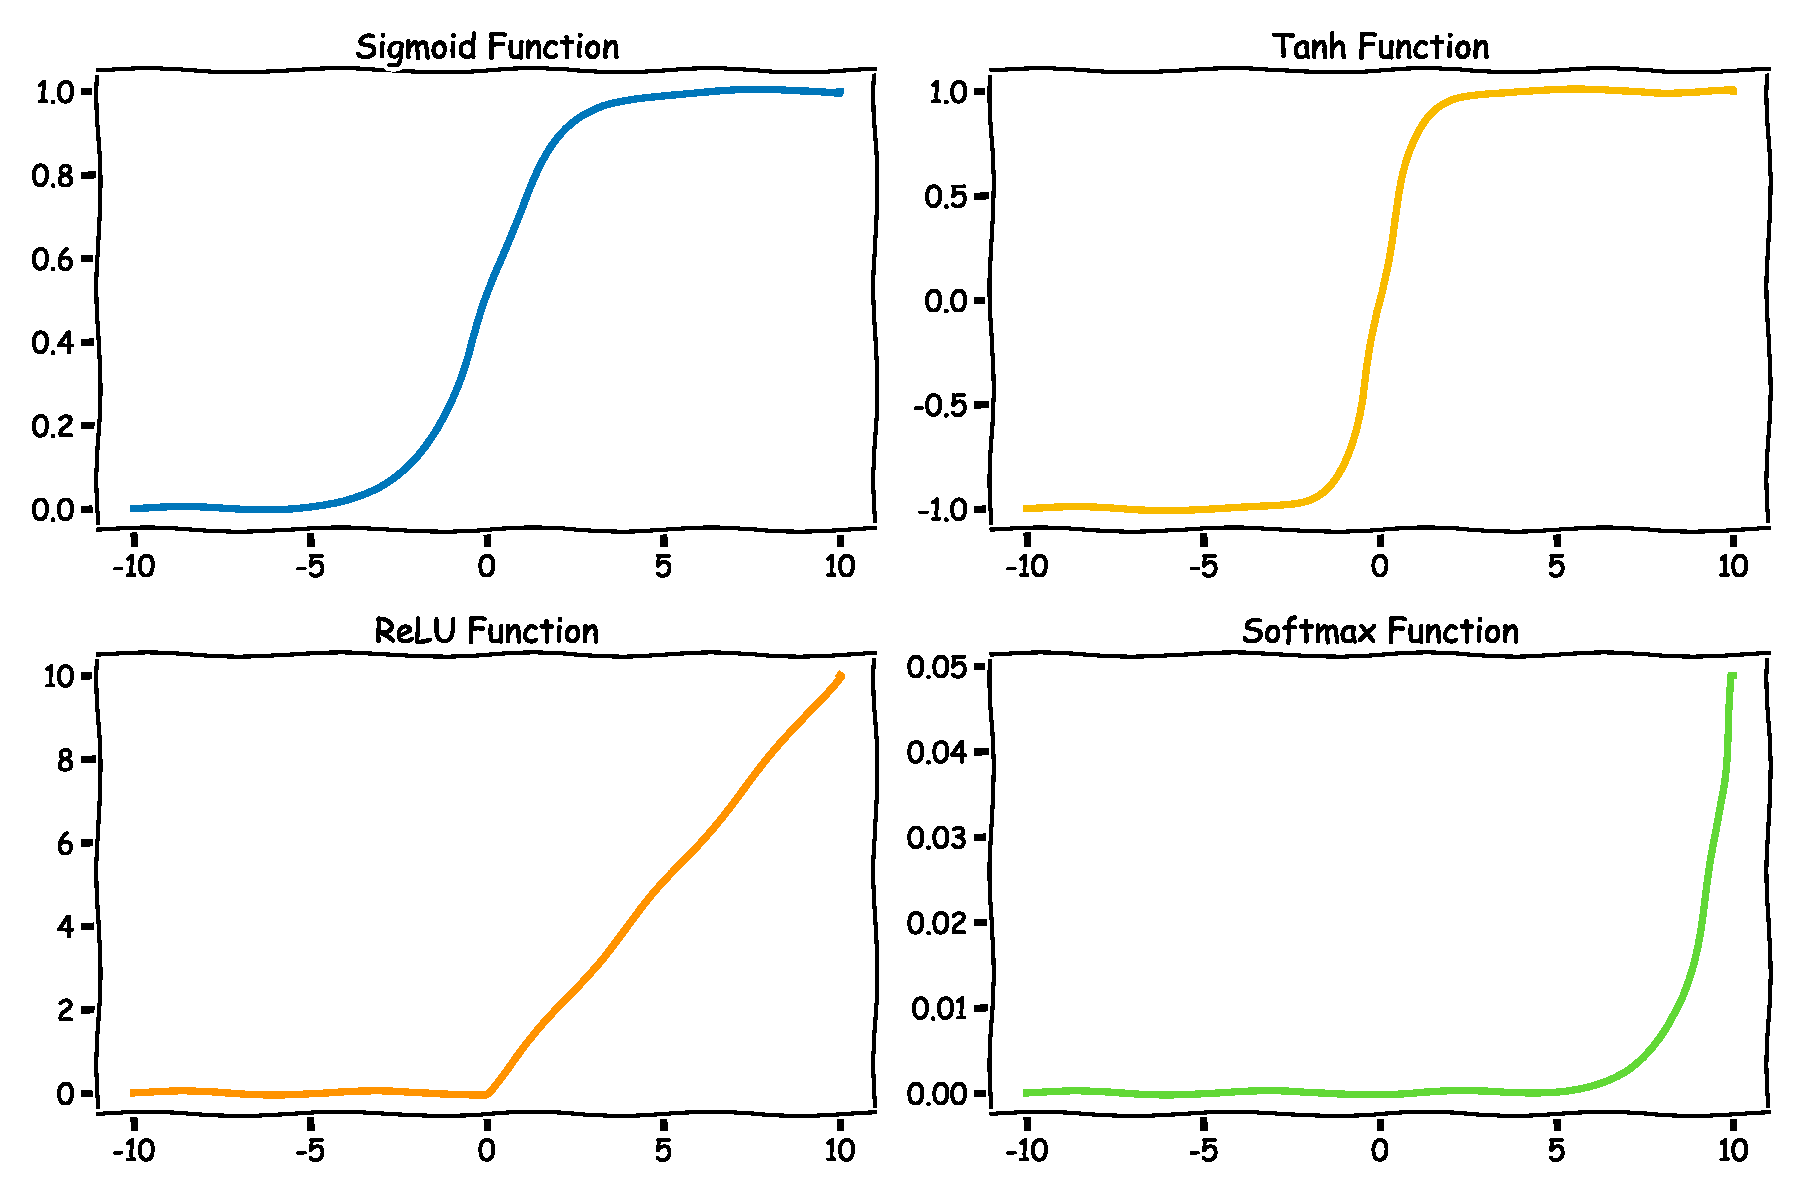
\includegraphics[width=1\linewidth]{LateX//figs/activation_functions_xkcd.pdf}
    \caption{Behavior of four common activation functions: Sigmoid, Tanh, ReLU, and Softmax.}
    \label{fig:activation-functions}
\end{figure}

In a neural network, the activation function is very important, because it decides how data moves through the layers. One of the most popular activation functions is the Rectified Linear Unit (ReLU). It became widely used after showing great results in the AlexNet model \cite{NIPS2012_c399862d}.

ReLU is particularly popular because it introduces non-linearity without saturating for positive values, an issue that affects functions like Sigmoid and Tanh, which tend to have very small gradients at extreme values, leading to the vanishing gradient problem. Additionally, the simplicity of ReLU’s derivative allows for efficient back-propagation, enhancing computational speed during training and supporting convergence in deep networks.
\begin{equation}
    f'(\textit{net}_i) =
    \begin{cases}
    1, & \textit{net}_i > 0 \\
    0, & \textit{net}_i \leq 0
    \end{cases}
\end{equation}
Given the importance of ReLU and its advantageous properties, this function will be the focus in subsequent sections, as it will serve as the primary activation function in the architectures discussed.

\subsection{Neural Network Architecture}
Neural networks are structured in layers, as shown in Figure~\ref{fig:nn-architecture}, which are described as follows::
\begin{itemize}
    \item \textit{Input Layer}: Takes in the raw data features;
    \item \textit{Output Layer}: Outputs the final predictions;
    \item \textit{Hidden Layers}: Contain intermediate neurons that extract hierarchical features. The presence of multiple hidden layers makes the network \textit{deep}, giving rise to deep neural networks (DNNs).
\end{itemize}
\begin{figure}[H]
    \centering
    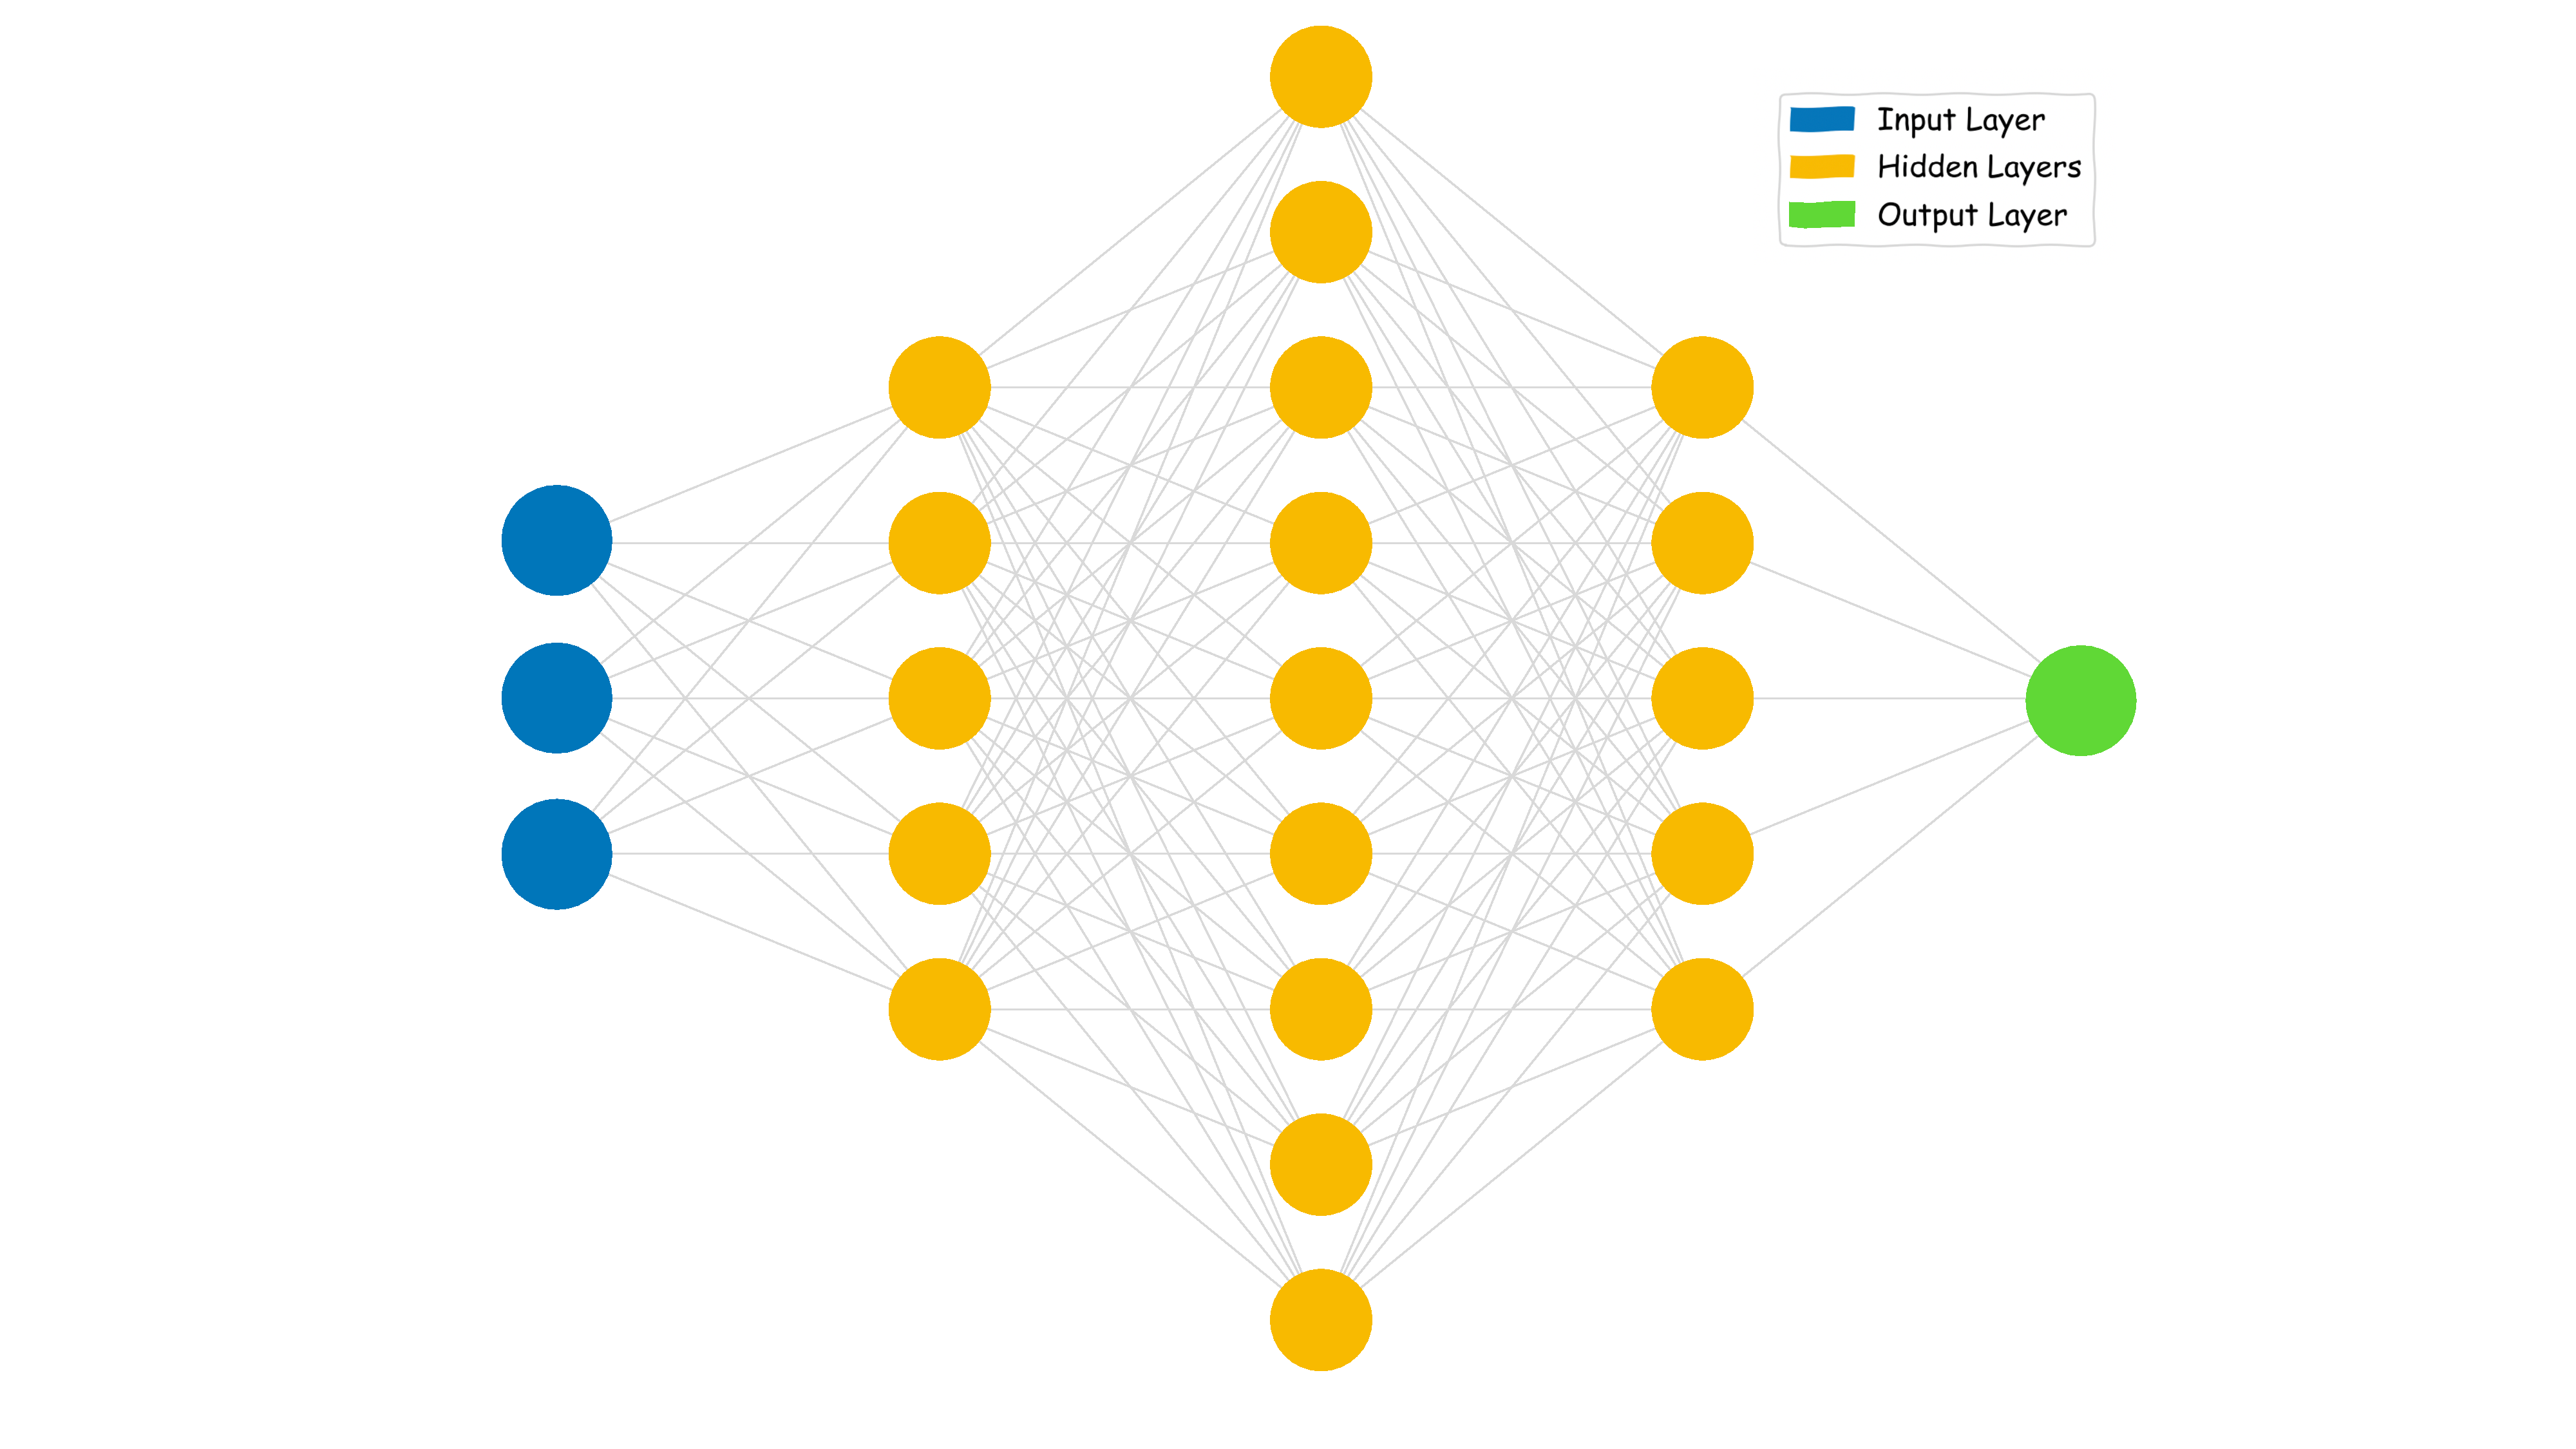
\includegraphics[width=0.75\linewidth]{LateX//figs/nn_intro_def.pdf}
    \caption{An illustration of a neural network architecture showing the input layer, hidden layers, and output layer.}
    \label{fig:nn-architecture}
\end{figure}

\subsubsection*{Forward Propagation}
Once the network architecture is defined, information propagates from the input layer to the output layer in a process called \textit{forward propagation}. This involves feeding inputs through each layer, applying the weights, summing them, and computing outputs using activation functions. The forward pass determines the final output for a given input.

\subsubsection*{Training Neural Networks}
The goal of training a neural network is to find the optimal set of weights $w_{ji}$ that map inputs to desired outputs. This process involves minimizing the difference between the network’s predictions and the actual targets, as measured by a \textit{loss function}.
Loss functions are a fundamental component of neural network training. They quantify the difference between the network's predictions and the true targets, guiding the network’s weight adjustments to reduce this difference. In essence, the loss function measures the \textit{error} of the network's predictions, with the goal of minimizing this error to improve the network's accuracy.

Depending on the task the neural network (NN) needs to learn, various loss functions can be used. Below are some widely used loss functions \cite{LF_review}:

\begin{itemize}
    \item \textit{L1 Loss}:  
    The L1 Loss calculates the absolute difference between the predicted and true values:
    \begin{equation}
        E(\mathbf{w}, \mathbf{x}) = \sum_{i=1}^{N} |y_i - \hat{y}_i|
    \end{equation}
    Here, \(y_i\) represents the true label, \(\hat{y}_i\) the predicted output, and \(N\) the number of samples. L1 Loss is robust to outliers because it does not square the error, reducing sensitivity to large differences.

    \item \textit{Mean Absolute Error (MAE)}:  
    MAE is derived from the L1 loss by calculating the mean of the absolute differences:
    \begin{equation}
        E(\mathbf{w}, \mathbf{x}) = \frac{1}{N} \sum_{i=1}^{N} |y_i - \hat{y}_i|
    \end{equation}
    Like L1 loss, it is robust to outliers and is widely used in regression tasks.

    \item \textit{L2 Loss}:  
    L2 loss computes the sum of squared differences between predicted and true values:
    \begin{equation}
        E(\mathbf{w}, \mathbf{x}) = \sum_{i=1}^{N} (y_i - \hat{y}_i)^2
    \end{equation}
    By squaring the errors, L2 loss is more sensitive to larger errors, which can be useful in tasks that require penalizing significant deviations but can be affected by outliers.

    \item \textit{Mean Squared Error (MSE)}:  
    MSE extends L2 loss by calculating the average of squared differences:
    \begin{equation}
        E(\mathbf{w}, \mathbf{x}) = \frac{1}{N} \sum_{i=1}^{N} (y_i - \hat{y}_i)^2
    \end{equation}
    It is commonly used in regression tasks but shares the sensitivity of L2 loss to outliers.

    \item \textit{Smooth L1 Loss}:  
    Smooth L1 loss blends L1 and L2 losses, making it less sensitive to outliers while retaining sensitivity to small errors:
    \begin{equation}
        E(\mathbf{w}, \mathbf{x}) = 
        \begin{cases} 
            0.5 \cdot (y_i - \hat{y}_i)^2 & \text{if } |y_i - \hat{y}_i| < \beta \\
          |y_i - \hat{y}_i| - 0.5 & \text{otherwise.}
        \end{cases}
    \end{equation}
    This loss is widely used in tasks like object detection, where robustness to outliers is important.

    \item \textit{Cross-Entropy Loss}:  
    Cross-entropy loss is commonly used in classification tasks. It measures the difference between the predicted probability distribution and the true distribution:
    \begin{equation}
        E(\mathbf{w}, \mathbf{x}) = -\frac{1}{N} \sum_{i=1}^{N} \sum_{c=1}^{C} y_{i,c} \log(\hat{y}_{i,c})
    \end{equation}
    Here, \(C\) is the number of classes, \(y_{i,c}\) is 1 if sample \(i\) belongs to class \(c\), and \(\hat{y}_{i,c}\) is the predicted probability for that class \cite{mao2023crossentropylossfunctionstheoretical}.

    \item \textit{Focal Loss}:  
    Focal loss extends cross-entropy loss with a modulating factor to focus more on hard-to-classify examples and address class imbalance:
    \begin{equation}
        E(\mathbf{w}, \mathbf{x}) = -\frac{1}{N} \sum_{i=1}^{N} \sum_{c=1}^{C} \alpha_c (1 - \hat{y}_{i,c})^\gamma y_{i,c} \log(\hat{y}_{i,c})
    \end{equation}
    Here, \(\alpha_c\) is a weighting factor for class \(c\), and \(\gamma\) controls the focus on difficult examples \cite{DBLP:journals/corr/abs-1708-02002}.

    \item \textit{IoU Loss}:  
    Intersection over Union (IoU) loss is used in object detection tasks to directly optimize the overlap between predicted and ground-truth bounding boxes. It is defined as:
    \begin{equation}
        E(\mathbf{w}, \mathbf{x}) = 1 - \frac{\text{Intersection}}{\text{Union}}
    \end{equation}
    The intersection is the area of overlap between the predicted and ground-truth bounding boxes, while the union is the combined area of both.

\end{itemize}

From now on, only the L1, L2, MSE, and MAE loss functions will be considered, as the task involved with this project is not focused on classification. Each of these loss functions offers unique advantages: L1 and smooth L1 are more robust to outliers, while MSE and L2 give greater penalty to larger errors. Choosing the right loss function is essential and should be based on the specific requirements of the task and the nature of the data. The behavior and comparison of these loss functions are illustrated in Figure~\ref{fig:loss-functions}.
\begin{figure}[H]
    \centering
    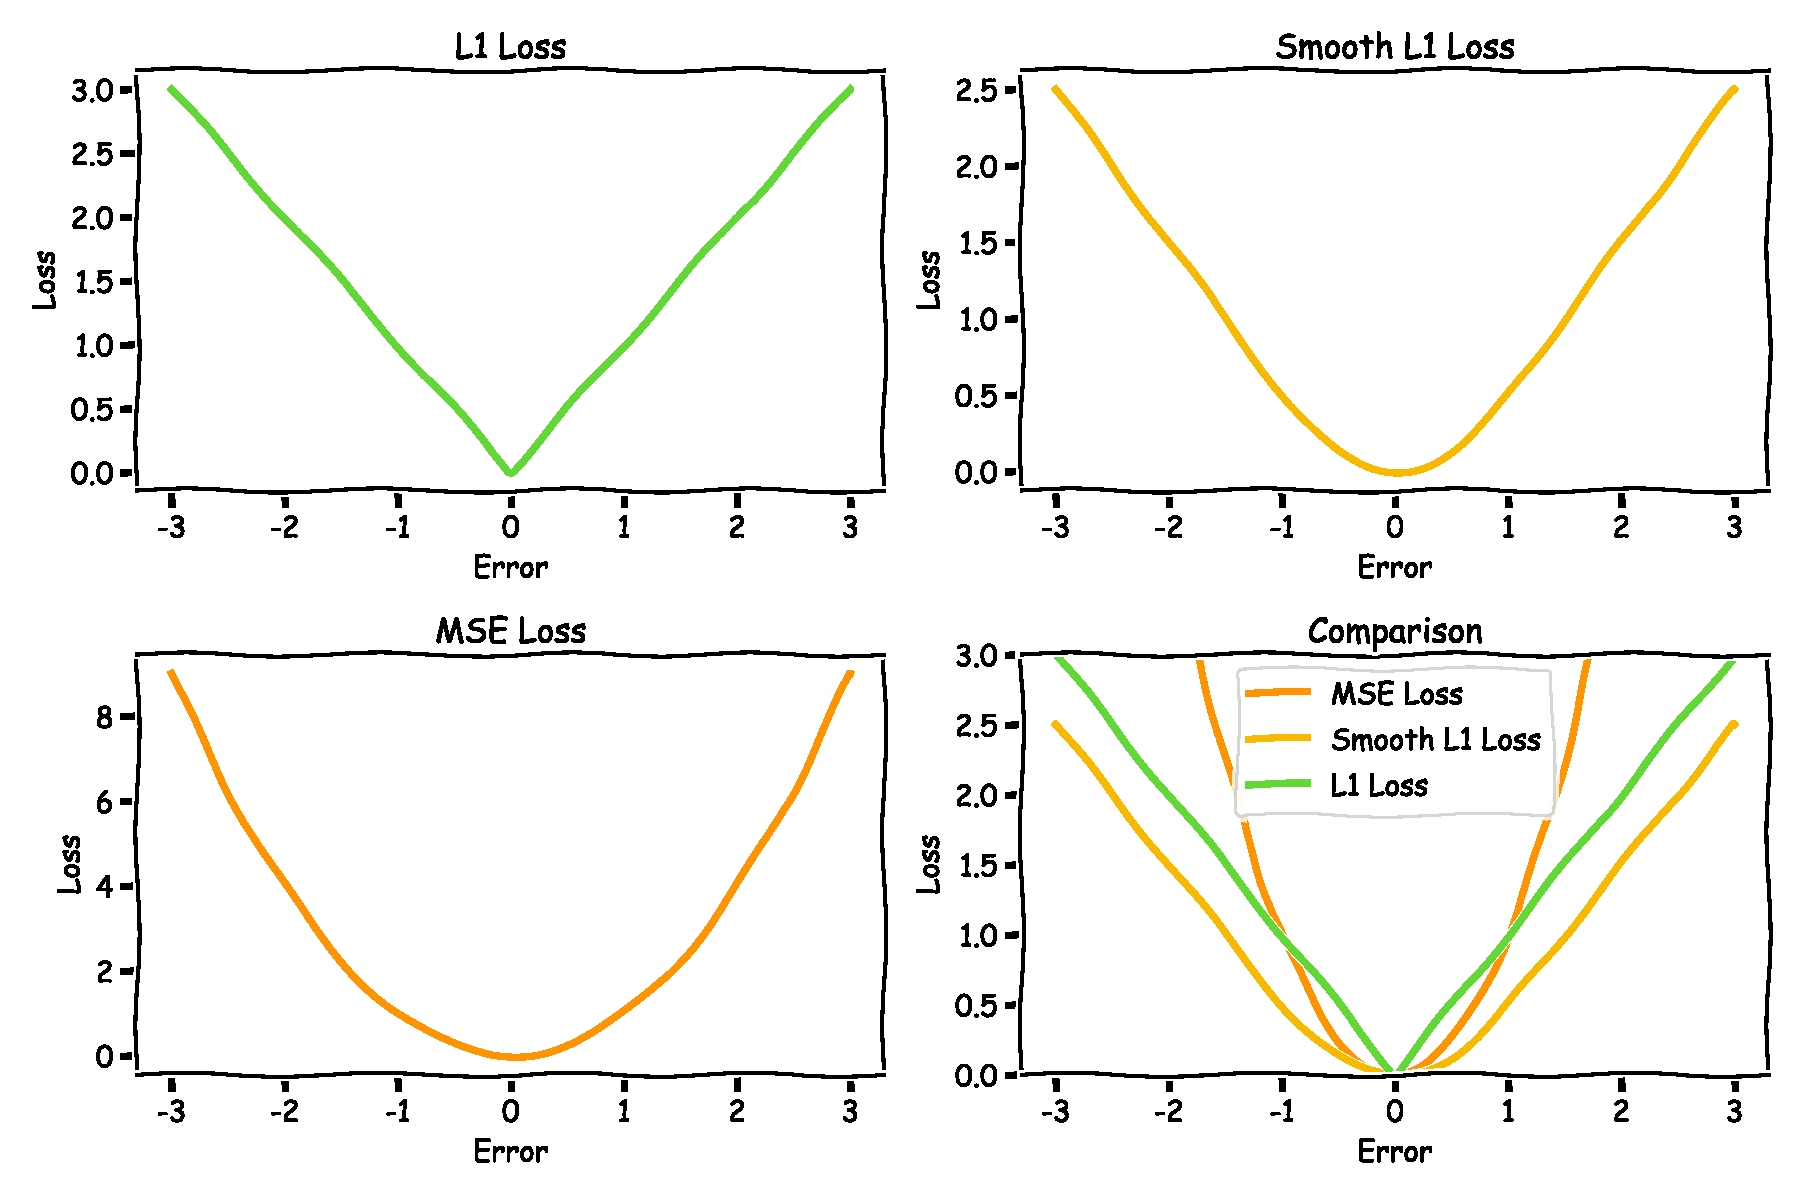
\includegraphics[width=1\linewidth]{LateX/figs/loss_functions_xkcd.pdf}
    \caption{Visualization of L1, Smooth L1, MSE, and a comparison of their behavior, highlighting their distinct characteristics.}
    \label{fig:loss-functions}
\end{figure}

\subsubsection*{Gradient Descent and Back-propagation}
In neural networks, after computing the gradients via \textit{back-propagation}, the following step is to update the weights to minimize the loss function. This is done using an optimizer, which controls how the weights are adjusted based on the gradients. The learning rate $\eta$ is a key hyper-parameter in this update process, determining the step size in the direction of the gradient. 
A proper learning rate is crucial: if it's too large, the network may overshoot the optimal solution; if it's too small, convergence becomes slow and inefficient, as shown in Figure ~\ref{fig:lr-behaviours}.
\begin{figure}[H]
    \centering
    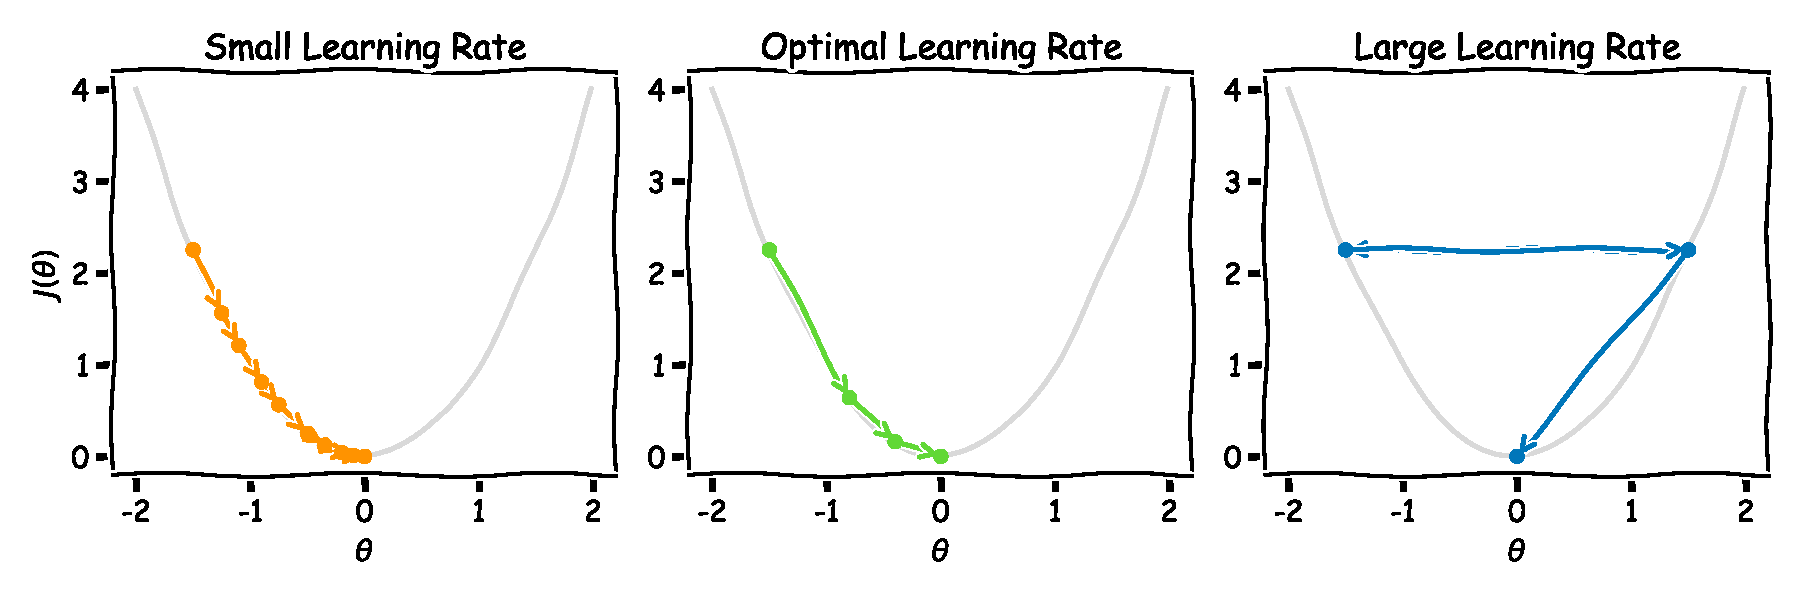
\includegraphics[width=1\linewidth]{LateX//figs/learning_rate.pdf}
    \caption{Illustration of the impact of different learning rates on the convergence behavior of gradient descent. A high learning rate can lead to overshooting the optimal solution, while a low learning rate results in slow convergence.}
    \label{fig:lr-behaviours}
\end{figure}

The optimizer updates the weights accordingly the following general rule:
\begin{equation}
    \theta \leftarrow \theta - \eta \nabla_\theta L
\end{equation}
where where: $\theta$ represents the weights, $\eta$ depicts the learning rate and $\nabla L_\theta$ is the gradient of the loss function with respect to the weights. 
\begin{equation}
    \nabla_\theta L = \frac{\partial L}{\partial \theta}
\end{equation}

Gradient Descent is an optimization algorithm that updates the model's parameters after analyzing the entire training dataset in each iteration. While this method ensures a comprehensive update, it is time-consuming, especially because the learning rate, a small value by design, results in only tiny adjustments to the parameters during each step. This makes training a neural network slow and inefficient. To address this issue, more efficient approaches have been developed. Two of the most widely used optimizers are Stochastic Gradient Descent (SGD), which updates parameters using small, randomly selected subsets of data (batches), and Adam, which combines adaptive learning rates with momentum to speed up convergence. These methods significantly improve training efficiency and are commonly used in modern deep learning.

\subsubsection*{Stochastic Gradient Descent}
A practical variant of gradient descent, particularly suited for large datasets, is Stochastic Gradient Descent (SGD). Unlike traditional gradient descent, which computes the gradient over the entire dataset, SGD calculates the gradient for each individual data point.

Due to its noisy behavior and time requirements, an improved version was developed that processes a small subset of the dataset, known as a mini-batch, for each iteration. This approach updates the weights after each mini-batch, introducing some randomness into the process while significantly speeding up training, especially with large datasets. SGD is more likely to escape local minima and can lead to better generalization.
\begin{algorithm}[H]
\caption{Stochastic Gradient Descent (SGD)}
\begin{algorithmic}[1]
\State \textbf{Initialize:} weights $\theta_{ih}, \theta_{ho}, \eta$, batch size $B$, max epochs $T_{\text{max}}$
\State $t \gets 0$

\Repeat
    \State $t \gets t + 1$
    \State $L \gets 0$ \Comment{Initialize loss}
    \State Randomly shuffle the training set $\mathcal{D}$

    \For {each mini-batch $\mathcal{B}$ of size $B$}
        \State Reset gradient: $\nabla \theta_{ih} \gets 0, \nabla \theta_{ho} \gets 0$
        
        \For {each sample $x_i$ in $\mathcal{B}$}
            \State \textbf{Forward step:} $y_i \gets \text{forward}(x_i, \theta_{ih}, \theta_{ho})$
            \State Compute loss $L \gets L + \mathcal{L}(y_i, t_i)$
            
            \State \textbf{Backward step:} Compute gradients $\nabla \theta_{ho}, \nabla \theta_{ih}$ 
        \EndFor

        \State Update hidden-output weights: $\theta_{ho} \gets \theta_{ho} - \eta \cdot \nabla \theta_{ho}$
        \State Update input-hidden weights: $\theta_{ih} \gets \theta_{ih} - \eta \cdot \nabla \theta_{ih}$
        
        \State $L \gets L / B$ \Comment{Average the loss}
    \EndFor
    
\Until {(not convergence \textbf{and} $t < T_{\text{max}}$)}

\end{algorithmic}
\end{algorithm}

\subsubsection*{Adam}
Another popular optimizer, especially in deep learning, is the Adam (short for Adaptive Moment Estimation) optimizer. Adam combines the benefits of both momentum and adaptive learning rates. It calculates individual adaptive learning rates for each parameter by considering both the first moment (the mean) and the second moment (the uncentered variance) of the gradients.
\begin{equation}
    \theta_t = \theta_{t-1} - \eta \cdot \frac{\hat{m}_t}{\sqrt{\hat{v}_t} + \epsilon}
\end{equation}
In the formula: \(\theta_t\) is the updated weight, \(\theta_{t-1}\) is the previous weight, \(\eta\) is the learning rate, \(\hat{m}_t\) is the bias-corrected first moment estimate, \(\hat{v}_t\) is the bias-corrected second moment estimate, and \(\epsilon\) is a small constant to prevent division by zero.

\begin{algorithm}[H]
\caption{Adam Optimizer}
\begin{algorithmic}[1]
\State \textbf{Initialize:} weights \(\theta_{ih}, \theta_{ho}, \eta\), batch size \(B\), max epochs \(T_{\text{max}}\), \(\beta_1, \beta_2\), \(\epsilon\)
\State \(m_{ih} \gets 0, v_{ih} \gets 0, m_{ho} \gets 0, v_{ho} \gets 0\) \Comment{Initialize parameters}
\State \(t \gets 0\) \Comment{Initialize time-step}

\Repeat
    \State \(t \gets t + 1\)
    \State \(L \gets 0\) \Comment{Initialize loss}
    \State Randomly shuffle the training set \(\mathcal{D}\)

    \For {each mini-batch \(\mathcal{B}\) of size \(B\)}
        \State Reset gradients: \(\nabla \theta_{ih} \gets 0, \nabla \theta_{ho} \gets 0\)

        \For {each sample \(x_i\) in \(\mathcal{B}\)}
            \State \textbf{Forward step:} \(y_i \gets \text{forward}(x_i, \theta_{ih}, \theta_{ho})\)
            \State Compute loss \(L \gets L + \mathcal{L}(y_i, t_i)\)

            \State \textbf{Backward step:} Compute gradients \(\nabla \theta_{ho}, \nabla \theta_{ih}\)
        \EndFor

        \State Update first moment estimates: 
        \[
        m_{ih} \gets \beta_1 \cdot m_{ih} + (1 - \beta_1) \cdot \nabla \theta_{ih}, \quad m_{ho} \gets \beta_1 \cdot m_{ho} + (1 - \beta_1) \cdot \nabla \theta_{ho}
        \]
        \State Update second moment estimates: 
        \[
        v_{ih} \gets \beta_2 \cdot v_{ih} + (1 - \beta_2) \cdot (\nabla \theta_{ih})^2, \quad v_{ho} \gets \beta_2 \cdot v_{ho} + (1 - \beta_2) \cdot (\nabla \theta_{ho})^2
        \]
        \State Bias correction:
        \[
        \hat{m}_{ih} \gets \frac{m_{ih}}{1 - \beta_1^t}, \quad \hat{m}_{ho} \gets \frac{m_{ho}}{1 - \beta_1^t}
        \]
        \[
        \hat{v}_{ih} \gets \frac{v_{ih}}{1 - \beta_2^t}, \quad \hat{v}_{ho} \gets \frac{v_{ho}}{1 - \beta_2^t}
        \]

        \State Update weights: 
        \[
        \theta_{ih} \gets \theta_{ih} - \eta \cdot \frac{\hat{m}_{ih}}{\sqrt{\hat{v}_{ih}} + \epsilon}
        \]
        \[
        \theta_{ho} \gets \theta_{ho} - \eta \cdot \frac{\hat{m}_{ho}}{\sqrt{\hat{v}_{ho}} + \epsilon}
        \]

        \State \(L \gets L / B\) \Comment{Average the loss}
    \EndFor

\Until {(not convergence \textbf{and} \(t < T_{\text{max}}\))}

\end{algorithmic}
\end{algorithm}

In this section, the fundamental structure of neural networks has been introduced, focusing on their building blocks, including neurons, layers, and connections by discussing the forward pass. Here inputs are processed through hidden layers to produce an output, and the back-propagation process is used to adjust the weights based on the error calculated at the output.

The typical workflow for training a neural network using backpropagation \cite{10.11648/j.ajnna.20190501.12} involves the following steps:

\begin{enumerate} 
    \item Initialize the network by assigning random weights to all connections;
    \item Compute the activation of the hidden nodes using the input data and the weights of the connections between the input layer and the hidden layer;
    \item Compute the activation of the output nodes using the activations of the hidden nodes and the weights of the connections between the hidden layer and the output layer;
    \item Calculate the error at the output nodes by comparing the predicted outputs to the actual target values;
    \item Adjust the weights between the output layer and the hidden layer by propagating the error backward through the network;
    \item Propagate the error further back to the hidden layer and adjust the weights between the hidden layer and the input layer accordingly;
    \item Repeat this process iteratively, updating the weights until a convergence criterion is met, such as reaching a minimal error or completing a predefined number of epochs;
    \item Once the training is complete, use the final optimized weights to make predictions by computing the activations of the output nodes.
\end{enumerate}

This iterative process allows neural networks to learn from data and improve over time. In the following chapters, it will be explored how these principles are applied to more complex architectures and tasks, including their use in localization methods for autonomous driving.

\subsection{Convolutional Neural Network (CNN)}

A Convolutional Neural Network (CNN), or \textit{ConvNet}, is a specialized type of deep learning algorithm designed for tasks like image classification, object detection, and segmentation. CNNs have become integral to various applications, including autonomous vehicles, medical imaging, security systems, and facial recognition technologies \cite{DBLP:journals/corr/OSheaN15}. 

What sets CNNs apart from traditional neural networks is their ability to exploit the spatial structure of data—typically images—by arranging neurons in a manner inspired by the human visual cortex. The architecture is organized into layers, each contributing to feature extraction and decision-making. These include:

\begin{itemize}
    \item \textit{Convolutional layers:} Apply filters (kernels) to the input image, generating feature maps that highlight patterns such as edges, textures, or shapes;
    \item \textit{Pooling layers:} Reduce the spatial dimensions of feature maps through operations like max pooling or average pooling, thereby lowering computational requirements and mitigating over-fitting;
    \item \textit{Fully connected layers:} Occurring near the network's end, these layers connect every neuron to the previous layer's neurons and play a key role in decision-making, such as classifying an image into categories.
\end{itemize}

CNNs are particularly efficient at processing 2D data by replacing traditional matrix multiplications with convolutional operations. This design enables them to capture spatial hierarchies in image data, from low-level features like edges to high-level features such as objects and faces.

To investigate deeper and provide a more detailed understanding, the building blocks of a CNN are:
\begin{enumerate}
    \item \textit{Convolutional Layers:} These layers perform operations that are mathematically similar to convolutions, but in practice, the operation computed is a \textit{correlation}, defined as:
    \begin{equation}
        (f \star g)(x, y) = \sum_{m}\sum_{n}f(x + m, y + n) \cdot g(m, n)
    \end{equation}
    where \( f \) represents the input and \( g \) denotes the kernel (or filter). For a 2D image, this operation involves sliding a filter over the input image and computing the dot product between the filter and segments of the image, resulting in an \textit{activation map}, as shown in Figure~\ref{fig:cnn-layer}. The kernels are learnable parameters, enabling the CNN to automatically learn feature detectors for edges, textures, and more complex patterns. Each filter responds to a particular feature within the input, such as vertical edges or textures.
    
    \begin{minipage}{\linewidth}
    \begin{figure}[H]
        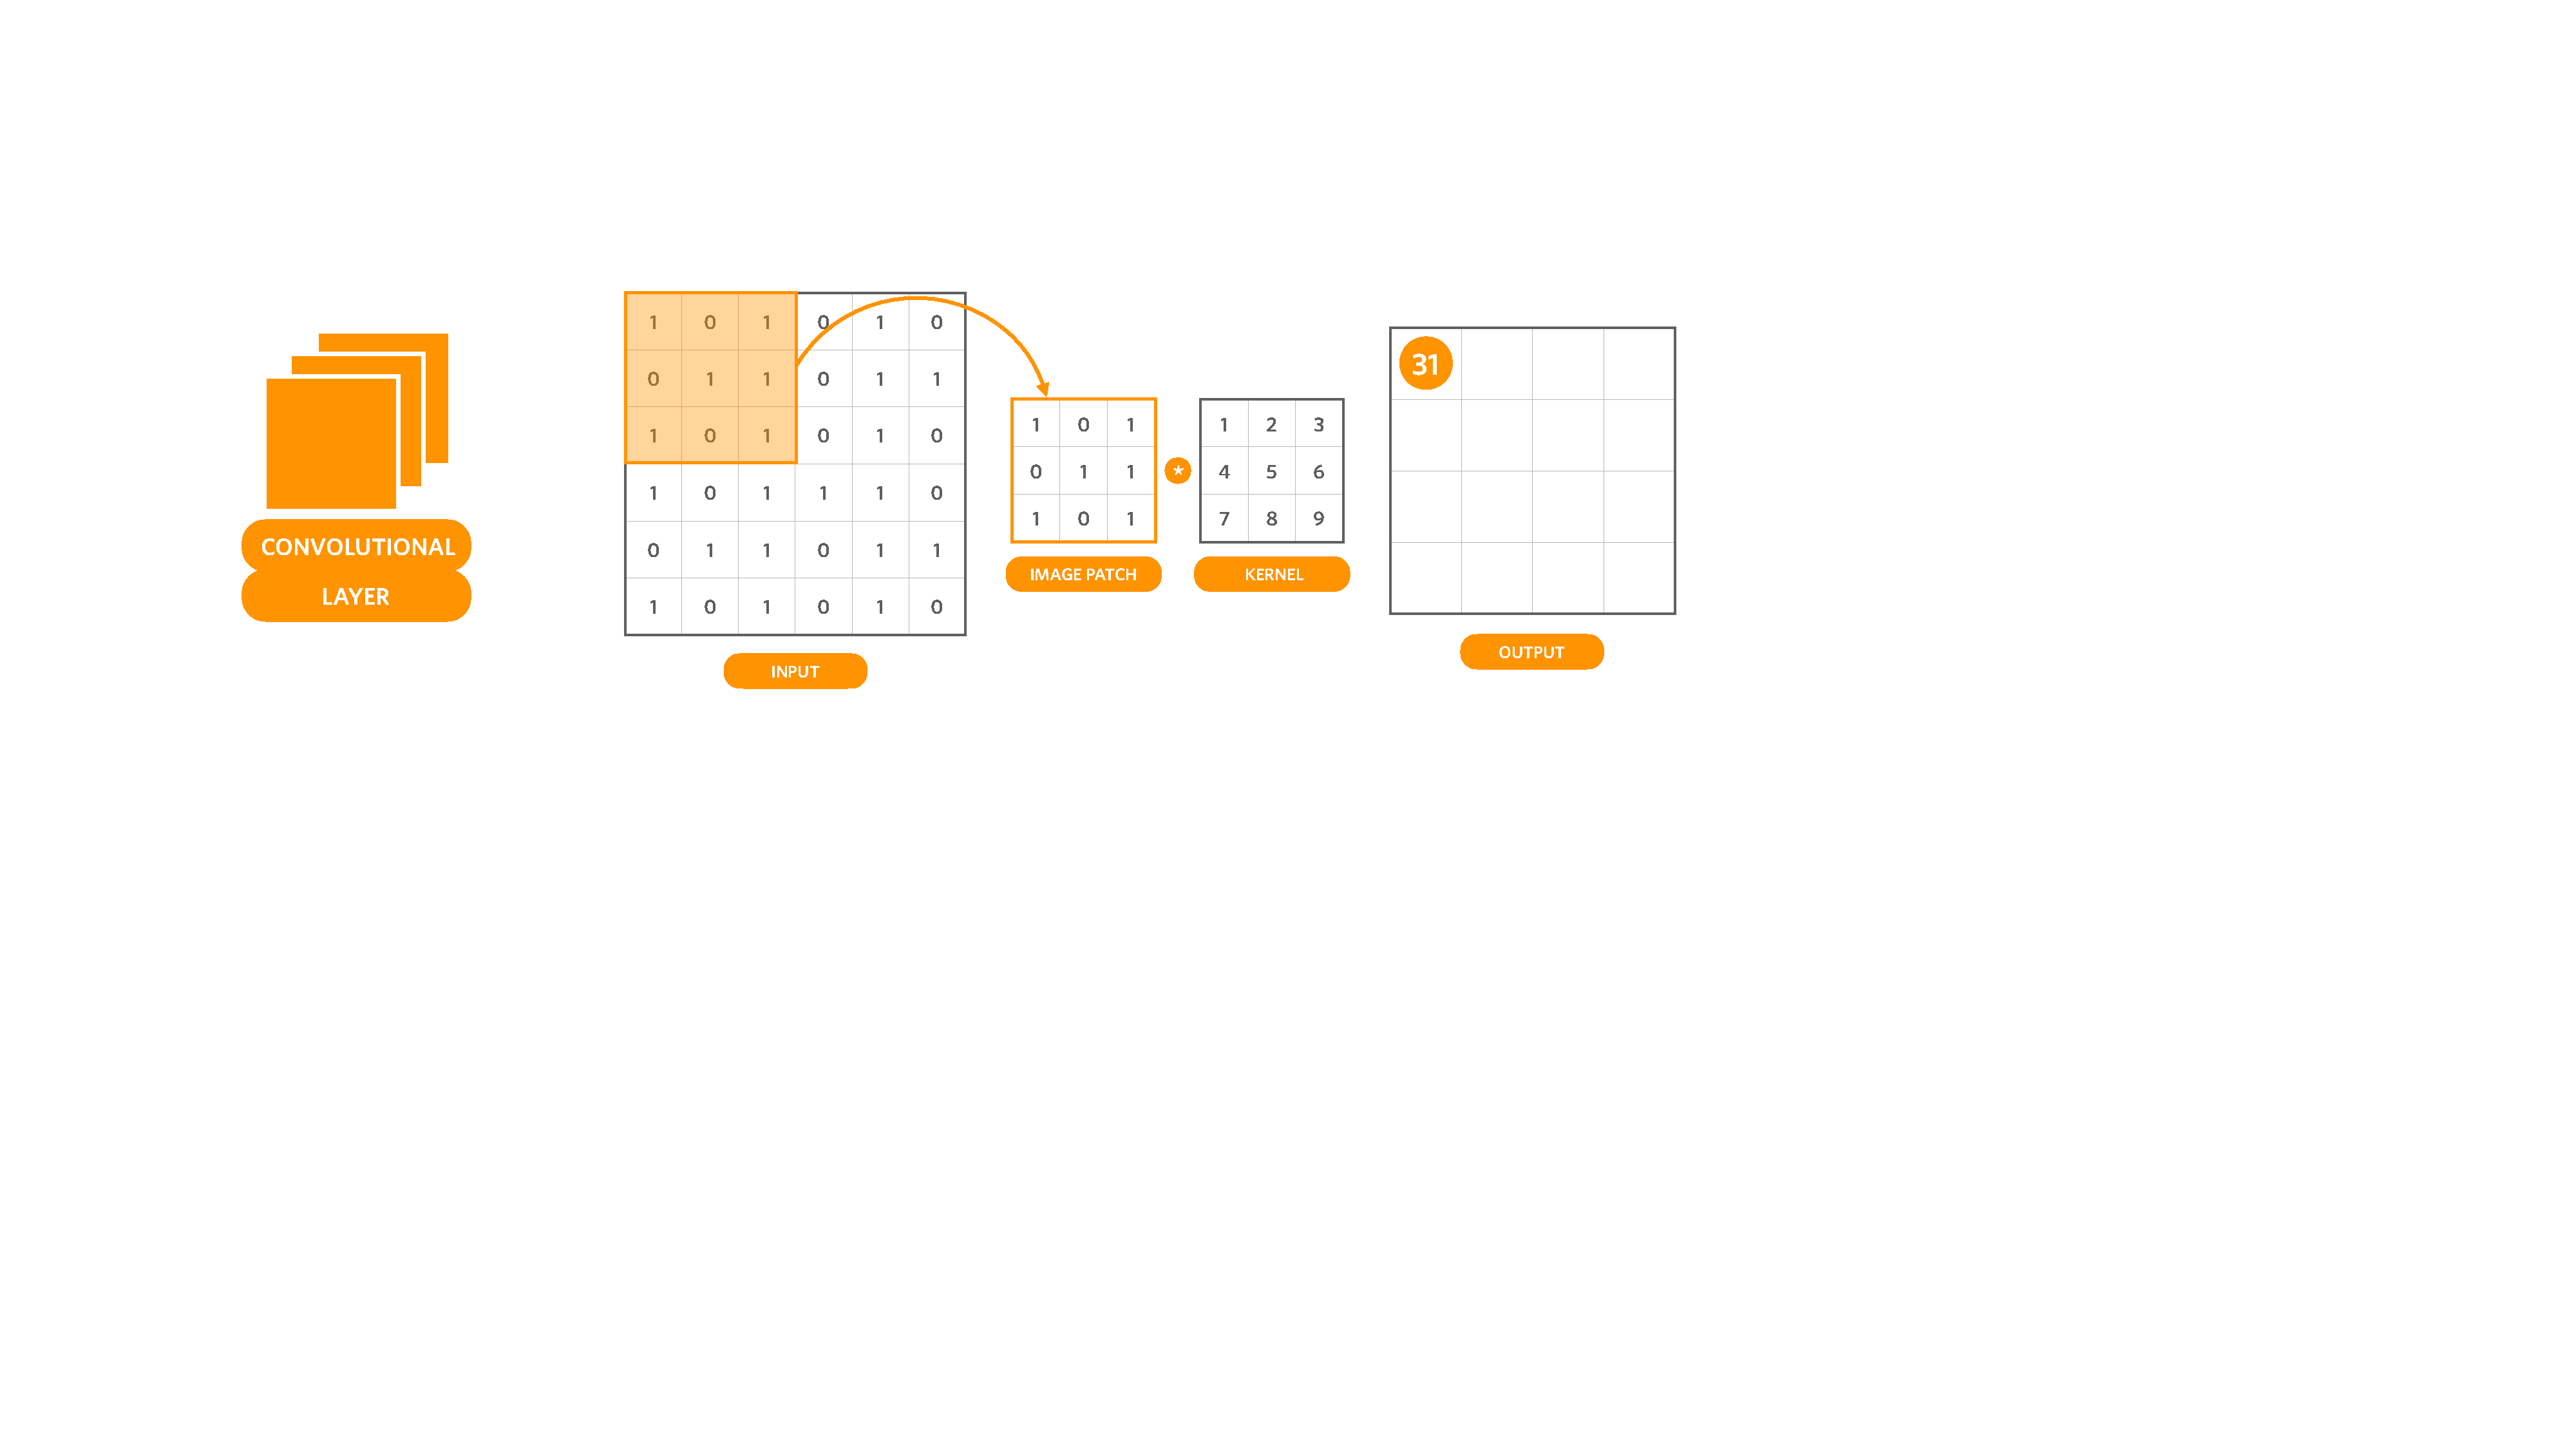
\includegraphics[width=1\linewidth]{LateX//figs/CCN_layer.pdf}
        \caption{Visualization of the operation of a Convolutional Layer. The diagram illustrates the input tensor, the selected patch, the learnable kernel, and the resulting output tensor.}
        \label{fig:cnn-layer}
    \end{figure}
    \end{minipage}
    \vspace{0.25 cm}
    
    Unlike fully connected (FC) layers, convolutional layers preserve the spatial (2D) structure of images, meaning the input and output are not flattened. Each output unit is connected only to a small, localized set of neighboring input units, known as the \textit{local receptive field}. Additionally, convolutional layers implement weight sharing, where the same weights are used across all positions of the input, ensuring that the same filter is applied throughout the image. This structure leverages the inherent properties of image data, where local patterns (e.g., edges or textures) often repeat in different locations across the image.

    \item \textit{Non-Linear Activation Function:} After the convolution operation, the next step is to apply a non-linear activation function to the resulting feature maps. This non-linearity enables the network to learn complex patterns and represent intricate relationships within the data. 

    \item \textit{Pooling Layers:} After the activation function, pooling layers are used to reduce the spatial dimensions of the activation maps while retaining the most important information. They aggregate neighboring values into a single output using a predefined function, applied channel-wise with a specific \textit{stride}. The \textit{stride} refers to the step size by which the pooling kernel moves across the input. A stride greater than 1 (\( s > 1 \)) results in down-sampling the activation map by skipping positions.
    
    The most commonly used pooling operation is \textit{max pooling}, which selects the maximum value from each patch of the feature map, as depicted in Figure~\ref{fig:cnn-pooling}. The mathematical formulation for max pooling is:
    \begin{equation}
        P = \max_{(i,j) \in \text{patch}} x(i,j)
    \end{equation}
    where \( P \) is the pooled value, and \( x(i,j) \) represents the values within the pooling window.
    
    \begin{minipage}{\linewidth}
    \begin{figure}[H]
        \centering
        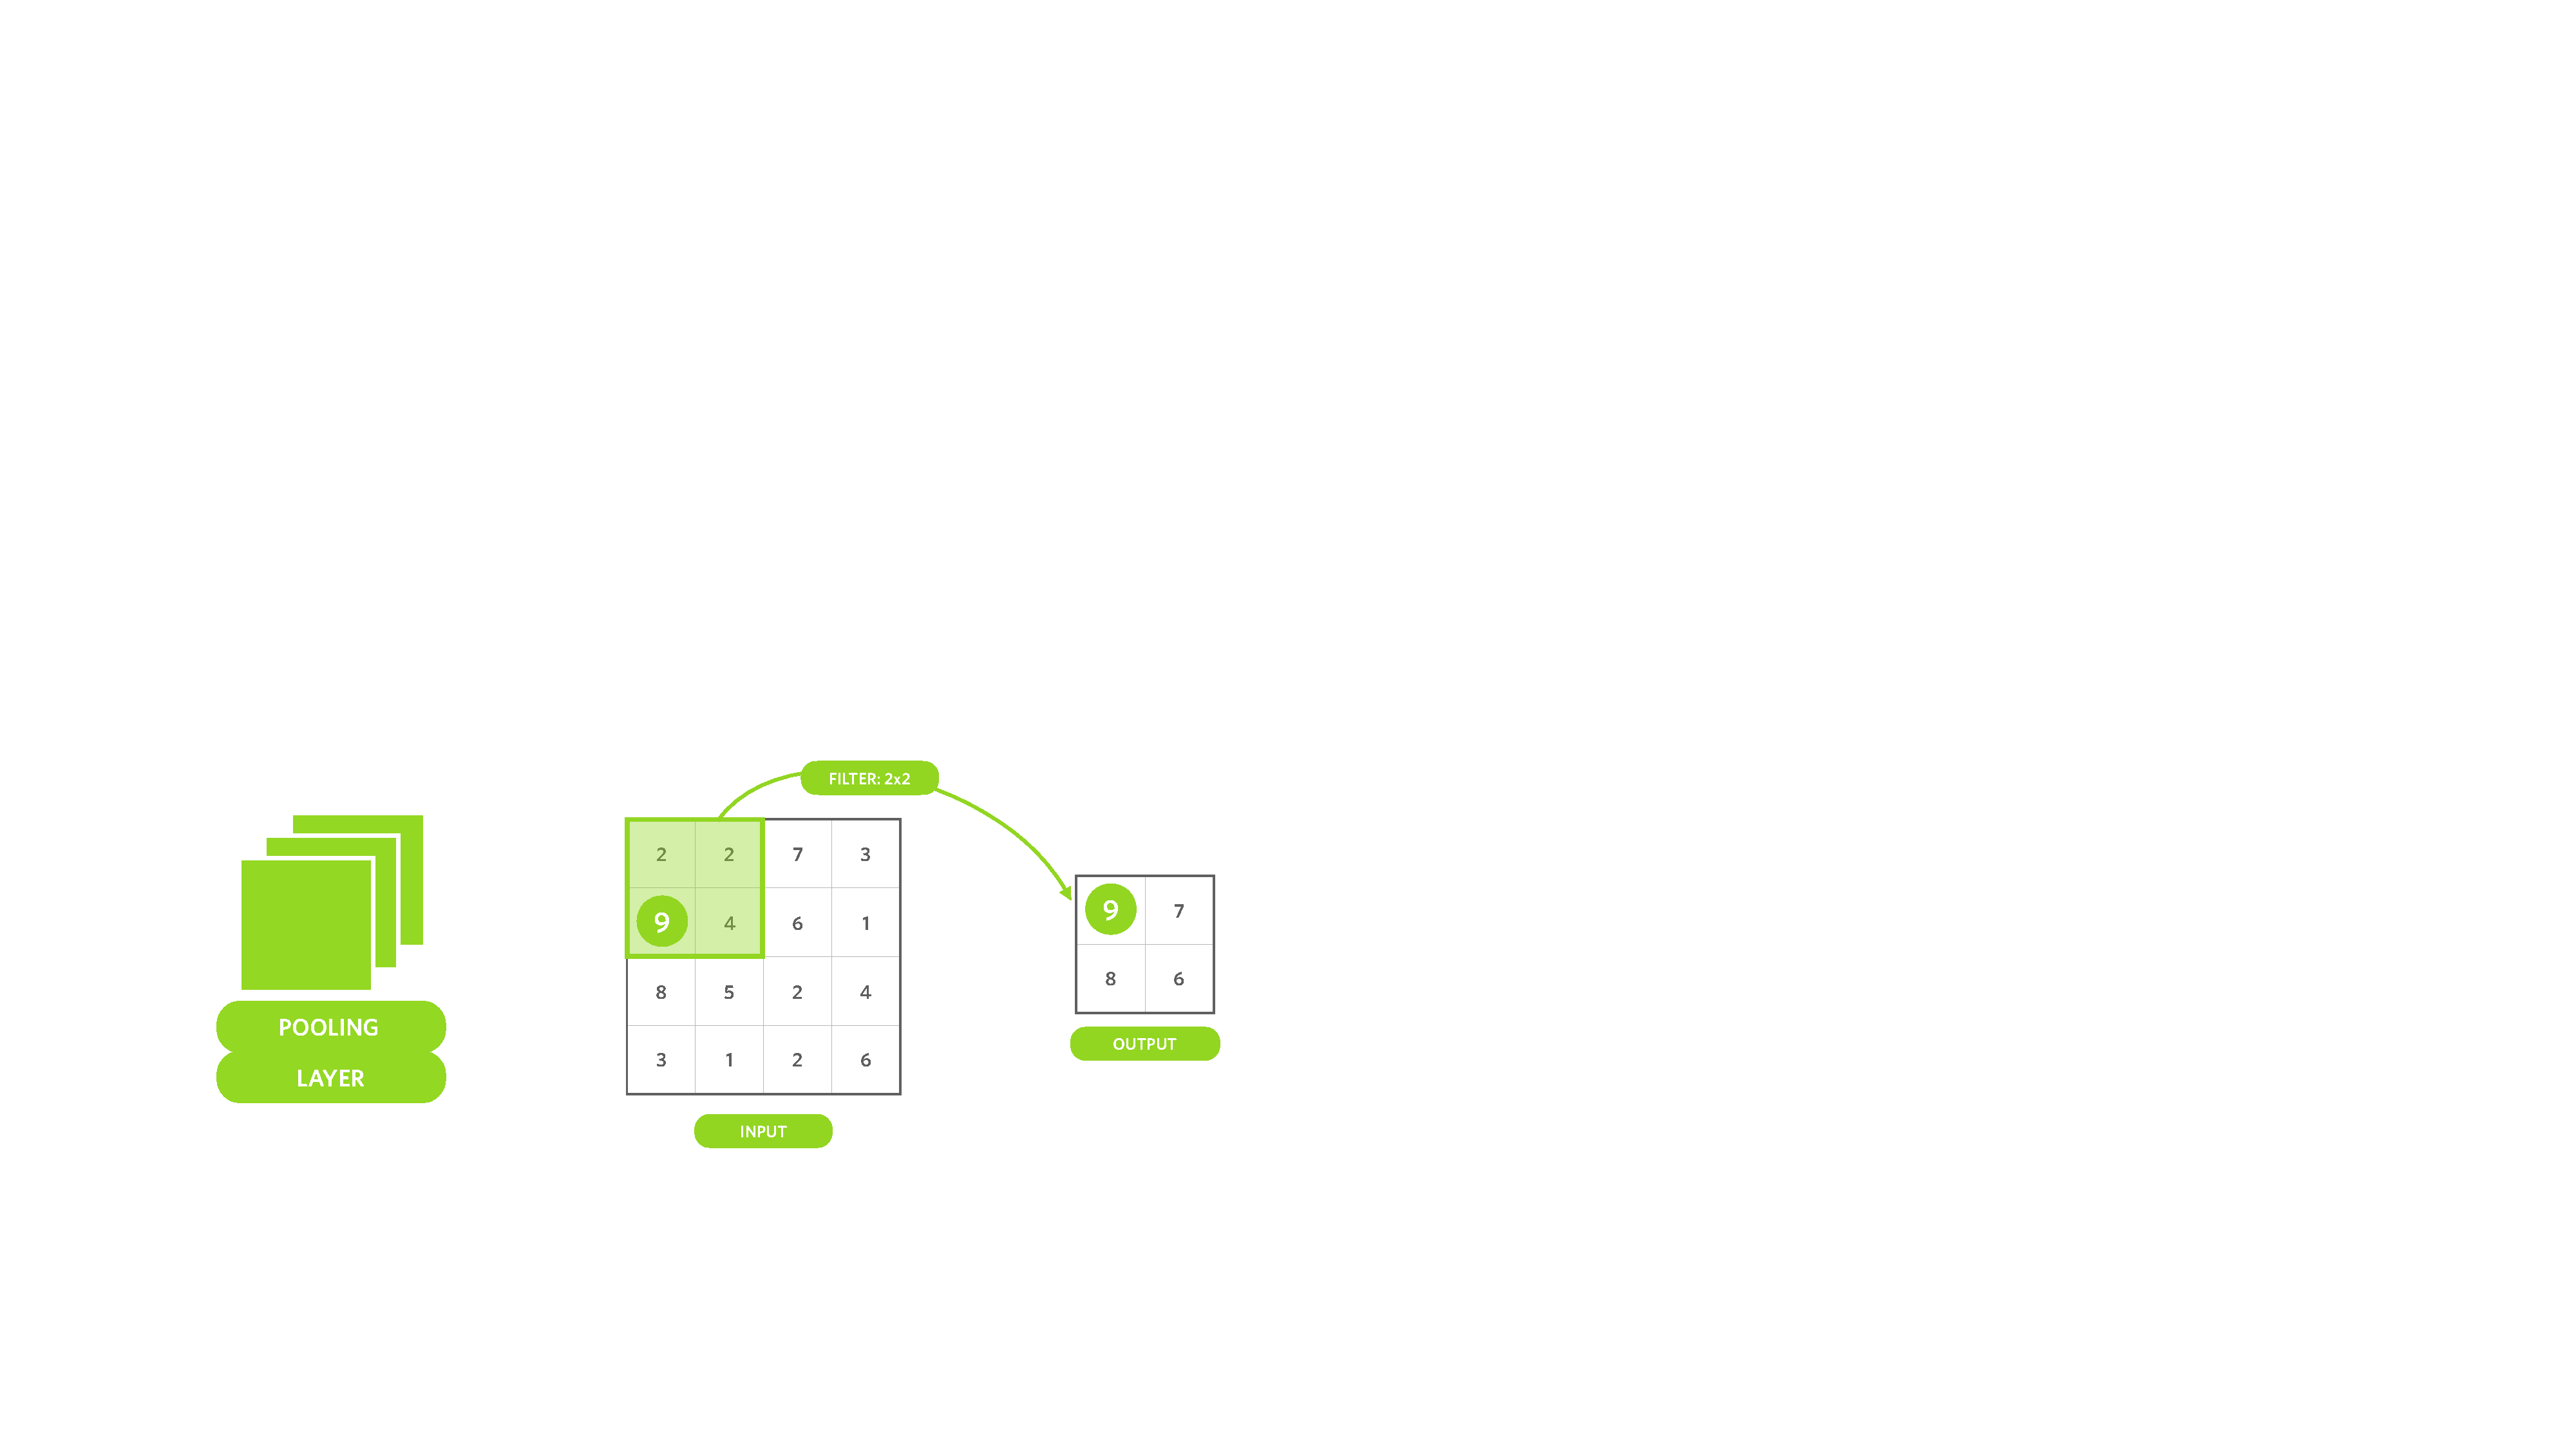
\includegraphics[width=0.85\linewidth]{LateX//figs/CNN_poolinh.pdf}
        \caption{Visualization of a Max-pooling Layer. The figure depicts the input tensor, the pooling window, and the resulting output tensor after applying the max-pooling operation.}
        \label{fig:cnn-pooling}
    \end{figure}
    \end{minipage}
    \vspace{0.25 cm}
    
    Pooling layers offer several benefits. They contribute to \textit{translation invariance}, making the network more robust to variations in the position or scale of features within the input. Notably, pooling layers do not have learnable parameters, which simplifies the network and reduces over-fitting. However, this lack of learnable parameters can also limit the network's ability to adapt pooling to specific tasks. 

    \item \textit{Fully Connected Layers:} In the final stage of a CNN, fully connected layers generate the network's output. These layers take the high-level features extracted by the previous layers and map them to the desired output format. Every neuron in a fully connected layer is connected to all neurons in the preceding layer, allowing the network to combine and interpret the features learned throughout the architecture. This step creates the final output, which could represent values such as predictions, scores, or any other required output specific to the task. A representation of a fully connected layer can be seen in Figure~\ref{fig:nn-architecture}.
    
\end{enumerate}

One of the key advantages of Convolutional Neural Networks (CNNs) over traditional machine learning models, such as Support Vector Machines (SVMs) or Decision Trees, is their ability to automatically learn features. Unlike traditional models that require manual feature extraction, CNNs autonomously learn hierarchical representations of data by employing multiple convolutional and pooling layers to extract features at various levels of abstraction.

CNNs are also commonly used as \textit{feature extractors} or \textit{backbones} in more complex neural network architectures. Their ability to automatically learn and generalize hierarchical features enables them to serve as powerful foundational networks that facilitate advanced tasks in various domains.

The main advantages of CNNs include:
\begin{itemize}
    \item \textit{Translation Invariance}: CNNs achieve translation invariance by applying the same convolutional filters across different parts of the image. This enables the network to recognize objects even when they appear in different locations within the image, which is a substantial advantage over traditional methods that often require manually engineered features.

    \item \textit{Hierarchical Feature Learning}: CNNs detect features in a hierarchical manner. In the initial layers, they capture low-level features such as edges, corners, or textures. In deeper layers, they detect higher-level, abstract features like shapes or object parts. This hierarchical learning process is akin to how the human visual cortex processes visual stimuli, progressing from simple to complex patterns.

    \item \textit{Efficiency}: By using local connectivity, each neuron in convolutional layers is connected only to a small region of the input, known as the \textit{receptive field}, rather than the entire input. This significantly reduces computational requirements. Additionally, weight sharing in convolution layers, where the same filter is applied across different regions, reduces the number of parameters compared to fully connected networks, making CNNs computationally efficient.
\end{itemize}

Over time, various CNN architectures have been developed to optimize performance for specific tasks. Notable architectures include:
\begin{enumerate}
    \item \textit{VGG-16}: Known for its simplicity, VGG-16 uses small \(3 \times 3\) convolutional filters but stacks a large number of convolutional layers followed by fully connected layers, creating a deep architecture with strong feature extraction capabilities \cite{7486599};

    \item \textit{ResNet}: ResNet introduced the concept of residual learning, which enables the training of very deep architectures. By incorporating skip connections, ResNet addresses the vanishing gradient problem, allowing for efficient training of deep networks. Various versions of ResNet exist, distinguished by the number of layers they contain, such as ResNet-18, ResNet-34, ResNet-50, ResNet-101, and ResNet-152. The number indicates the total layers, with deeper variants like ResNet-101 and ResNet-152 providing increasingly refined feature representations while maintaining efficient training \cite{DBLP:journals/corr/HeZRS15, 10197463};

    \item \textit{Inception (GoogLeNet)}: The Inception network incorporates convolutional layers of varying sizes applied in parallel. This multi-scale approach allows the network to capture features at different levels of granularity, enhancing its ability to recognize complex patterns \cite{DBLP:journals/corr/SzegedyLJSRAEVR14};

    \item \textit{EfficientNet}: This model family scales network width, depth, and resolution to achieve higher accuracy with fewer parameters. EfficientNet strikes a balance between accuracy and efficiency, making it a popular choice for many practical applications \cite{DBLP:journals/corr/abs-1905-11946}.
\end{enumerate}

While CNNs were originally designed for image-related tasks, their versatility has led to adaptations in various other domains, including:
\begin{itemize}
    \item \textit{Natural Language Processing (NLP)}: CNNs are used for tasks such as text classification by applying convolutional filters over word embeddings, allowing the network to capture local dependencies in textual data;

    \item \textit{Time Series Analysis}: CNNs can be applied to temporal data, effectively capturing local dependencies between data points over time, making them suitable for analyzing patterns in time series data;

    \item \textit{Speech Recognition}: In combination with Recurrent Neural Networks (RNNs) or Transformers, CNNs can be utilized in speech recognition tasks, such as voice recognition or speech-to-text conversion, where they contribute to feature extraction and processing.
\end{itemize}

Through these applications, CNNs have proven to be a flexible and powerful tool in both traditional and emerging fields, providing a foundation for extracting robust features that can enhance the performance of complex neural networks.

\subsection{Transformers}

While Convolutional Neural Networks (CNNs) excel at extracting spatial features from structured data like images, they are often insufficient when dealing with inputs that involve complex dependencies across long sequences or multiple modalities. CNNs are inherently limited by their local receptive fields and are not designed to capture global relationships effectively. This limitation becomes critical in tasks where the inputs have different modalities, such as combining textual, auditory, and visual data, or when understanding dependencies across sequences, such as in language processing.

The primary challenge in multimodal learning lies in representing and summarizing multimodal data to exploit the complementarity and redundancy of multiple modalities. The heterogeneity of multimodal data adds complexity to constructing such representations. For instance, language is often symbolic, while audio and visual modalities are represented as signals \cite{baltruvsaitis2018multimodal}.

Another significant challenge involves mapping data from one modality to another. Multimodal data relationships are often open-ended or subjective; for example, there can be multiple correct descriptions for an image, and a single perfect translation may not exist. Similarly, fusing information from multiple modalities to make predictions introduces further difficulties. For instance, in audio-visual speech recognition, visual lip motion must be combined with audio signals to predict spoken words, despite varying predictive power, noise levels, and the possibility of missing data \cite{baltruvsaitis2018multimodal}.

Transformers were initially developed to solve sequence transduction tasks, such as neural machine translation, where an input sequence is transformed into an output sequence. Examples include speech recognition and text-to-speech transformation. Unlike Recurrent Neural Networks (RNNs), which struggle with long-range dependencies due to information loss across long chains, transformers address these limitations by introducing self-attention mechanisms \cite{vaswani2017attention}.

The attention mechanism, introduced to overcome the bottleneck of fixed-length encoding vectors, enhances model capacity for handling long or complex sequences \cite{DBLP:journals/corr/VaswaniSPUJGKP17}. Attention can be formulated as:
\begin{equation}
    \text{Attention} = f(g(x), x)
\end{equation}
where \( g(x) \) generates attention, corresponding to identifying discriminative regions, and \( f(g(x), x) \) processes input \( x \) based on attention \( g(x) \).

Attention mechanisms can be categorized by their data domains:
\begin{itemize}
    \item \textit{What to attend to (channel):} Highlights specific features;
    \item \textit{Where to attend to (spatial):} Focuses on spatial regions;
    \item \textit{When to attend to (temporal):} Captures temporal dynamics.
\end{itemize}

As shown in Figure~\ref{fig:attention}, the architecture of the attention mechanism highlights the interaction between the input and the attention weights.
\begin{figure}[H]
    \centering
    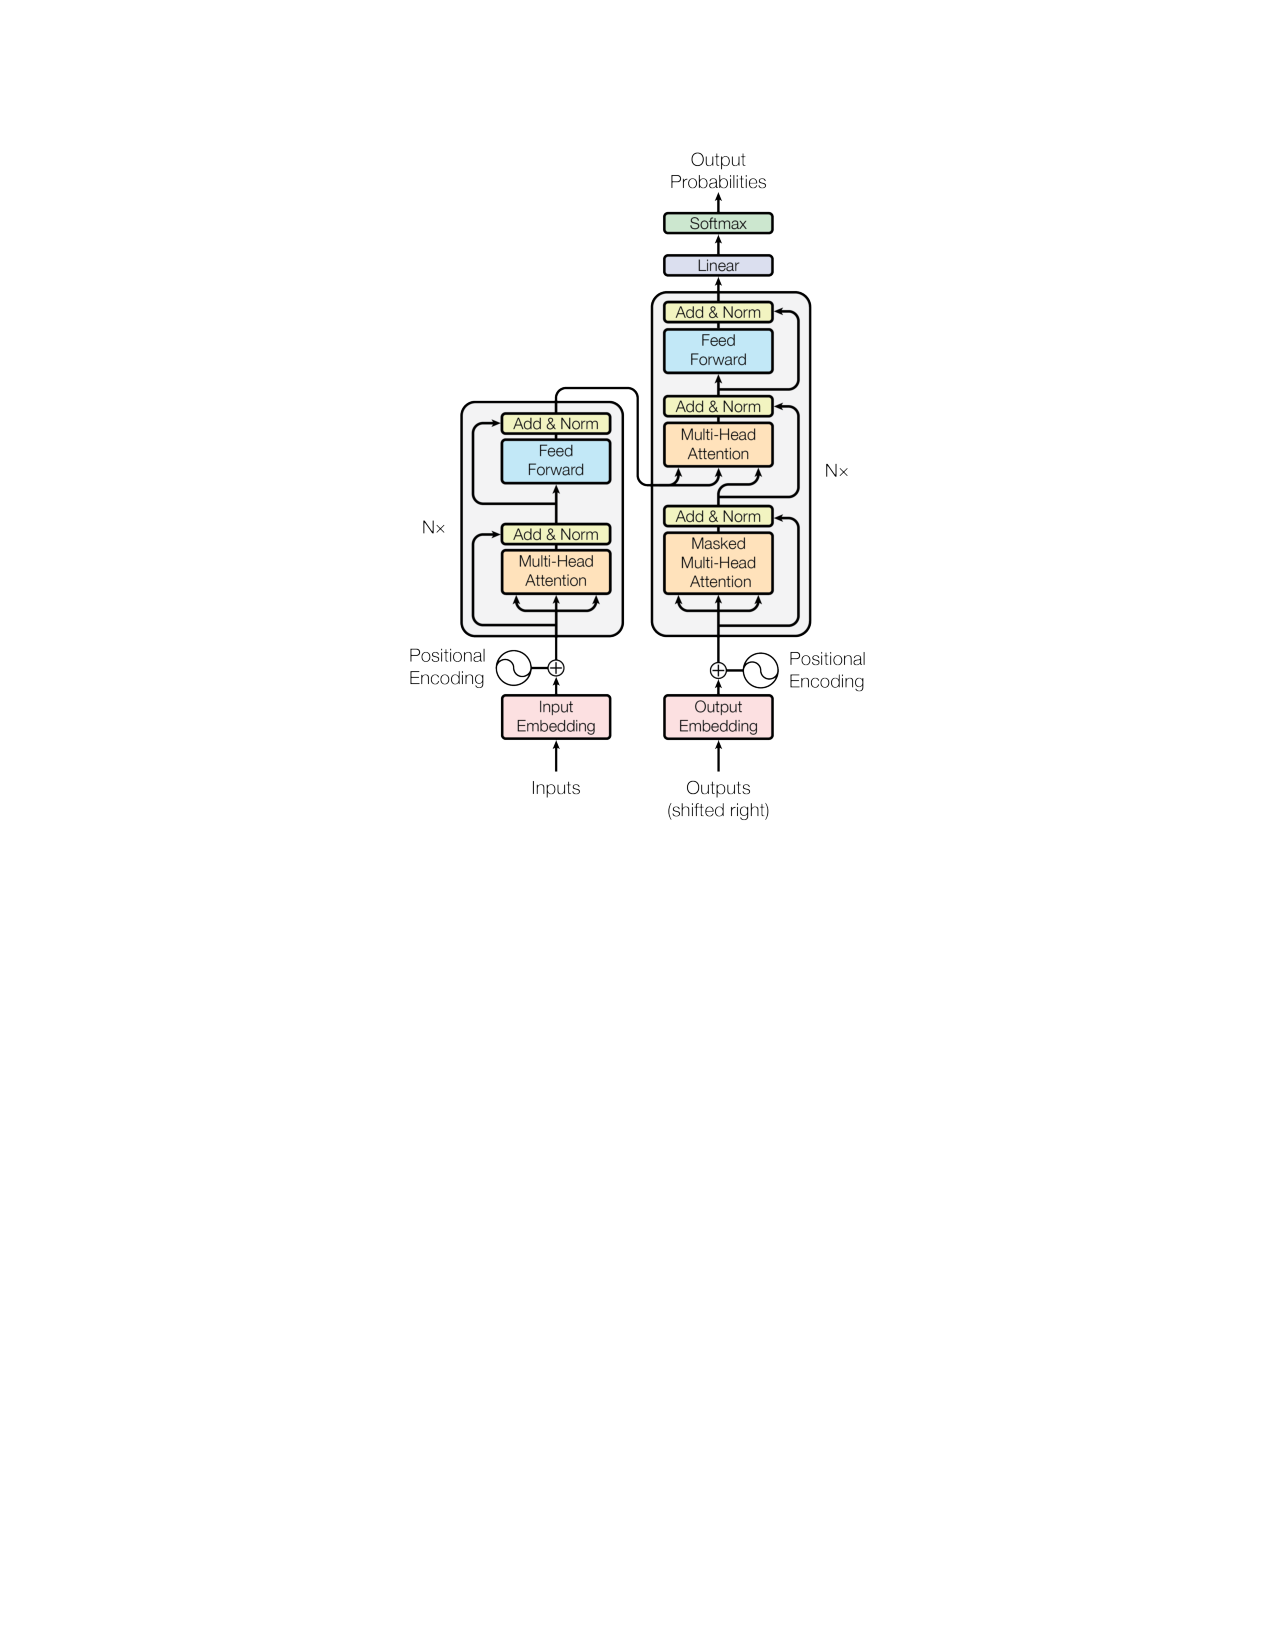
\includegraphics[width=0.5\linewidth]{LateX/figs/attention_transformer_architecture.pdf}
    \caption{Architecture of the attention mechanism \cite{DBLP:journals/corr/VaswaniSPUJGKP17}.}
    \label{fig:attention}
\end{figure}

Self-attention, the core of transformers, operates by transforming the input sequence into three vectors: queries, keys, and values. These are computed through linear transformations. The attention mechanism then calculates a weighted sum of the values based on the similarity between queries and keys. The weighted sum, combined with the original input, is processed through a feed-forward network to produce the output, enabling the model to capture long-range dependencies effectively \cite{ramachandran2019standalone}.

\section{MapAlign: Architecture description}
This section introduces MapAlign, the neural network developed in this thesis, following an initial overview of neural networks. MapAlign is designed to integrate smoothly into the pipeline of a deeper neural network, mentioned in Chapter 1, capable of reconstructing HD maps, starting from data gathered by the vehicle's onboard sensors, in Real Time.

MapAlign is positioned specifically at the dataset creation stage, addressing a critical challenge in the pipeline: achieving precise alignment between the vehicle's sensor data and the HD map, which serves as the target for the deeper network \cite{Li_HDMapNet_2022}. Traditional pipelines for HD map creation rely heavily on manual annotation and extensive resources to maintain map semantics, significantly limiting their scalability. In contrast, MapAlign automates the ground-truth generation process, minimizing reliance on optimization techniques and eliminating the need for manual alignment steps.

Creating a network that can reconstruct an HD map in real time by using image features from surrounding cameras or point clouds from radar, or other sensors, to predict vectorized map elements in a bird’s-eye view has many advantages. MapAlign helps this architecture, by eliminating the need for manual adjustments during ground truth generation. Additionally, better localization improves the accuracy and reliability of the generated HD map. This precise alignment not only accelerates the dataset creation process but also enhances the overall system’s performance, as improved alignment contributes to better accuracy in the deeper network's learning and predictions.


MapAlign’s primary objective is to output values that populate a rotation-translation matrix, aligning the HD map with the vehicle’s perception, by predicting the values of the three coordinates \( (x, y, z) \) and the heading angle \( \theta \), while contributions from pitch and roll are ignored, as they are unnecessary for this alignment task. These values define how to rotate and translate the map to match the vehicle's spatial understanding accurately. 

\subsection{Input Loaders}
Given the purpose of MapAlign, it is clear that this neural network requires input about the car's surroundings and the portion of the HD map corresponding to the vehicle's current position. These data can be either generated or, in this specific case, collected by autonomous vehicles equipped with extensive sensor suites that will be explained in more detail in the following sections.

The neural network processes data mainly stored in Python dictionaries, which are created by de-serializing binary files generated during the runs of the autonomous vehicle. These runs include both human-driven mode and autonomous driving mode when engaged. Before the network can use the data, it must be pre-processed to ensure proper formatting and compatibility with the network's requirements.

This subsection details the input loaders used in the system, focusing on how the network takes and prepares data for processing. The network operates with sensor data formatted as tensors, which are structured to resemble multi-channel images. In this representation, each point (analogous to a pixel in an image) contains specific information, while each channel corresponds to data from a particular sensor. 
The primary input loaders are:
\begin{itemize}
    \item \textit{BevObservation Loader:} This loader generates a tensor that encapsulates all Bird's-Eye View (BEV) measurements extracted from the data produced by detector neural networks installed on the vehicle. It processes data from the binary serialization file, organizing it into distinct channels, each corresponding to a specific data type, such as lane markings, road boundaries, free spaces, traffic signs, obstacles, stixels\footnote{A stixel is a compact representation of vertical structures in an environment, such as poles, pedestrians, or vehicles. It divides the scene into small vertical columns, summarizing 3D information into a simplified format for efficient processing.}, parking areas, and individual instances. The specific elements included in the tensor can be configured through a dedicated configuration file, allowing flexibility.
    In this architecture, the focus is primarily on \textit{road boundaries}. These are critical as they align closely with features present in high-definition (HD) maps, which are crucial for accurate map-to-sensor alignment.
    
    To create the multi-channel tensor, data from different sensors must be transformed into the same image coordinate system. This ensures that all channels can integrate smoothly. Each type of sensor data requires specific transformations and pre-processing. For camera data, because images are calibrated, through perspective projection images can be warped to match the BEV perspective. For radar data, the point cloud is filtered and projected onto the BEV tensor, taking into account the sensor's position and orientation.

    A visual representation of the multi-channel tensor is presented in Figure~\ref{fig:bev-loader}, where each layer is represented with a different color, illustrating the layered structure of the tensor.

    \begin{minipage}{\linewidth}
    \begin{figure}[H]
        \centering
        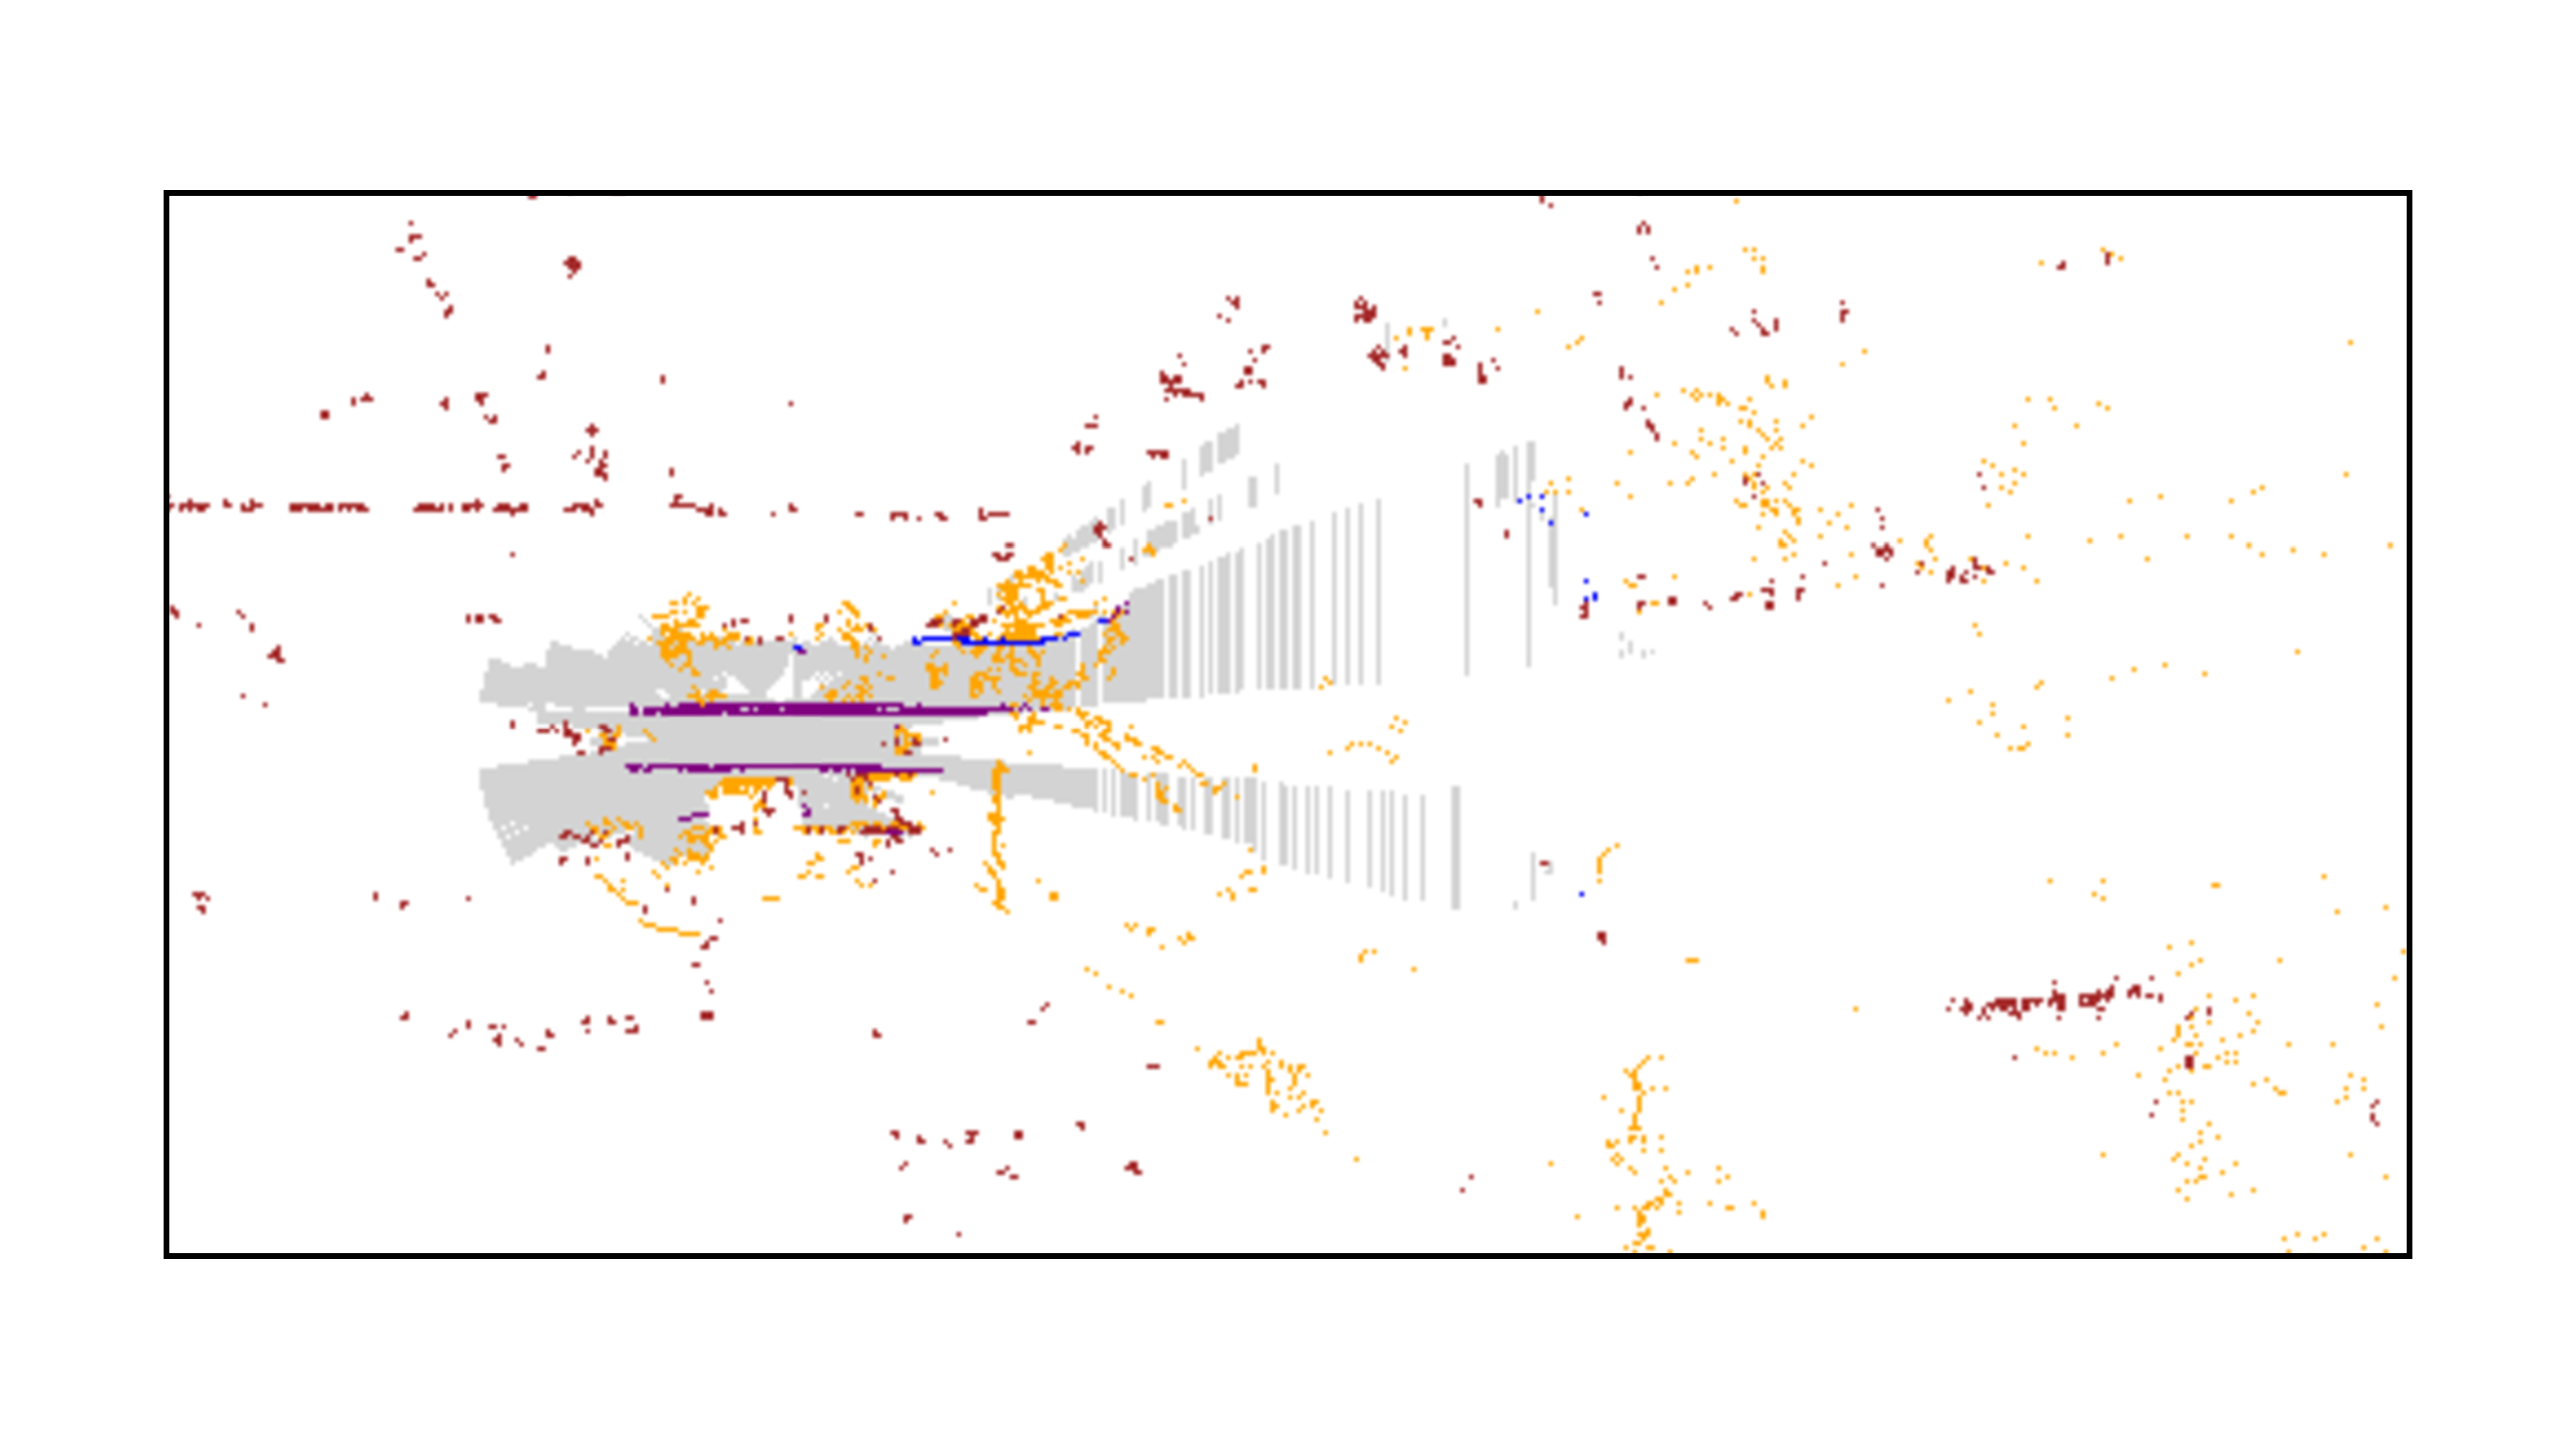
\includegraphics[width=0.85\linewidth]{LateX//figs/observations.pdf}
        \caption{Layered Tensor Representation of Sensor Inputs: Blue indicates curbs and lane markings, yellow represents the radar point cloud, red corresponds to stixels projections, and gray denotes free space.}
         \label{fig:bev-loader}
    \end{figure}
    \end{minipage}
    \vspace{0.25 cm}
    
    \item \textit{Ego Loader:} This component represents the ego vehicle within the same tensor used for other sensor data. A dedicated function generates a rectangular outline corresponding to the vehicle's physical dimensions. These dimensions are derived from the vehicle used to record the dataset sequences, ensuring accurate representation and alignment within the scene.
    The function takes as input the vehicle's specific spatial coordinates, including key points and orientations, with particular emphasis on the \textit{heading angle}, which defines the vehicle's direction relative to the map or environment frame. This precise representation is especially valuable for visualizations, enabling the ego vehicle's position and orientation to be clearly understood in relation to the surrounding environment.
    A visual representation of the ego vehicle's tensor overlay is shown in Figure~\ref{fig:ego-loader}, where the vehicle's rectangular outline is depicted within the BEV tensor.

    \begin{minipage}{\linewidth}
    \begin{figure}[H]
        \centering
        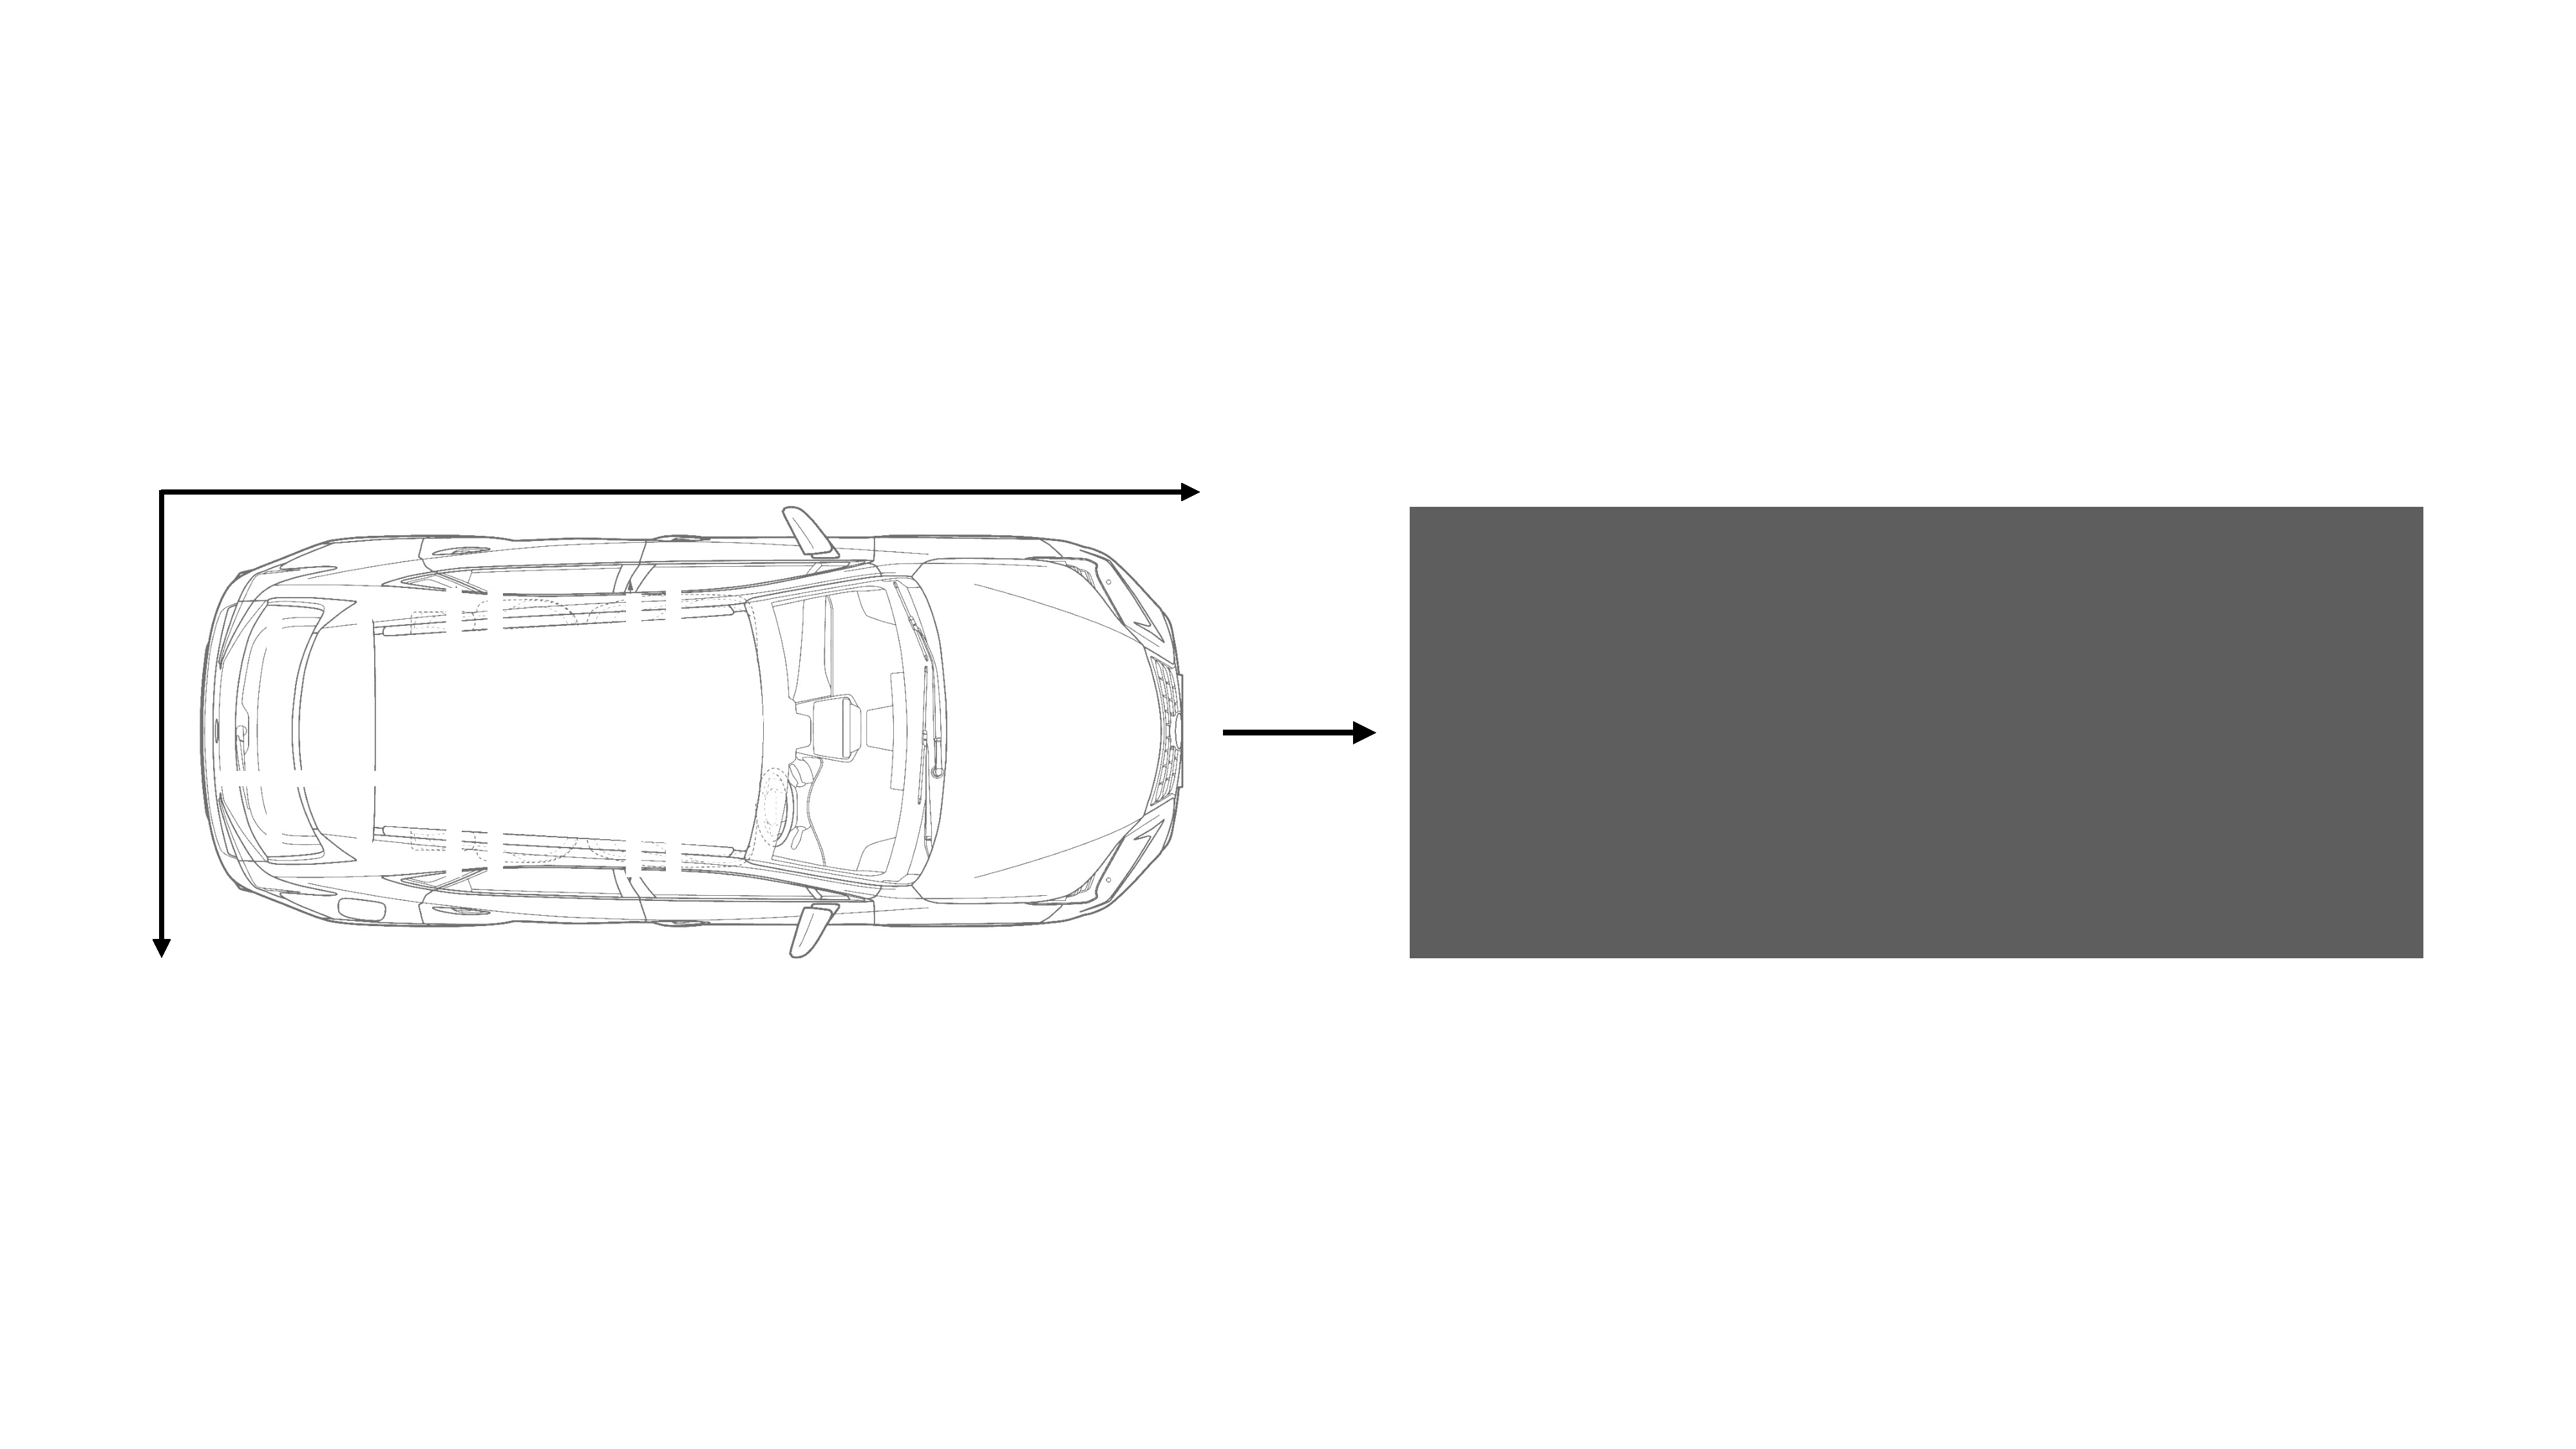
\includegraphics[width=0.75\linewidth]{LateX//figs/egoLoader.pdf}
        \caption{Tensor Representation of the Ego Vehicle: The dimensions of the car are represented as a rectangle mapped in tensor coordinates.}
        \label{fig:ego-loader}
    \end{figure}
    \end{minipage}
    \vspace{0.25 cm}
    
    \item \textit{Boundaries Loader:} This data loader generates a semantic representation of the operational environment's boundaries by creating a tensor that encodes this information. It takes as input a dictionary containing HD map data for the relevant area. The dimensions of the reference area are specified in a configuration file, defining the rectangular region around the vehicle's position used for boundary extraction.
    The map data uses a fixed spatial resolution to ensure precise alignment with the vehicle’s position, where each pixel corresponds to $25$ centimeters in the real world. To focus on the relevant area, the loader queries the map within a predefined region extending from $-32$ meters to $96$ meters along the $x$-axis and from $-32$ meters to $32$ meters along the $y$-axis, covering the vehicle’s operational zone. 
    To optimize computational efficiency, map compression reduces data density beyond a specific threshold. Within close proximity, the map’s resolution is preserved, while beyond $50$ meters along the x-axis and $20$ meters along the y-axis, data density is reduced. This ensures high-quality spatial data near the vehicle while maintaining computational efficiency.

    The tensor is initialized with zeros, indicating the absence of boundaries. Boundary points from the HD map are then drawn onto the tensor using OpenCV's \texttt{polyline} function \cite{itseez2015opencv}. The use of anti-aliased polylines (\texttt{LINE\_AA}) allows pixel values to range between $0$ and $1$, representing the probability of a boundary passing through a pixel, as illustrated in Figure~\ref{fig:polylines}. In this representation, a value of $0$ means no boundary is present in the pixel, a value of $1$ indicates that the boundary directly passes through the pixel, and intermediate values between $0$ and $1$ signify the probability of a boundary passing through the pixel.
    
    \begin{minipage}{\linewidth}
    \begin{figure}[H]
        \centering
        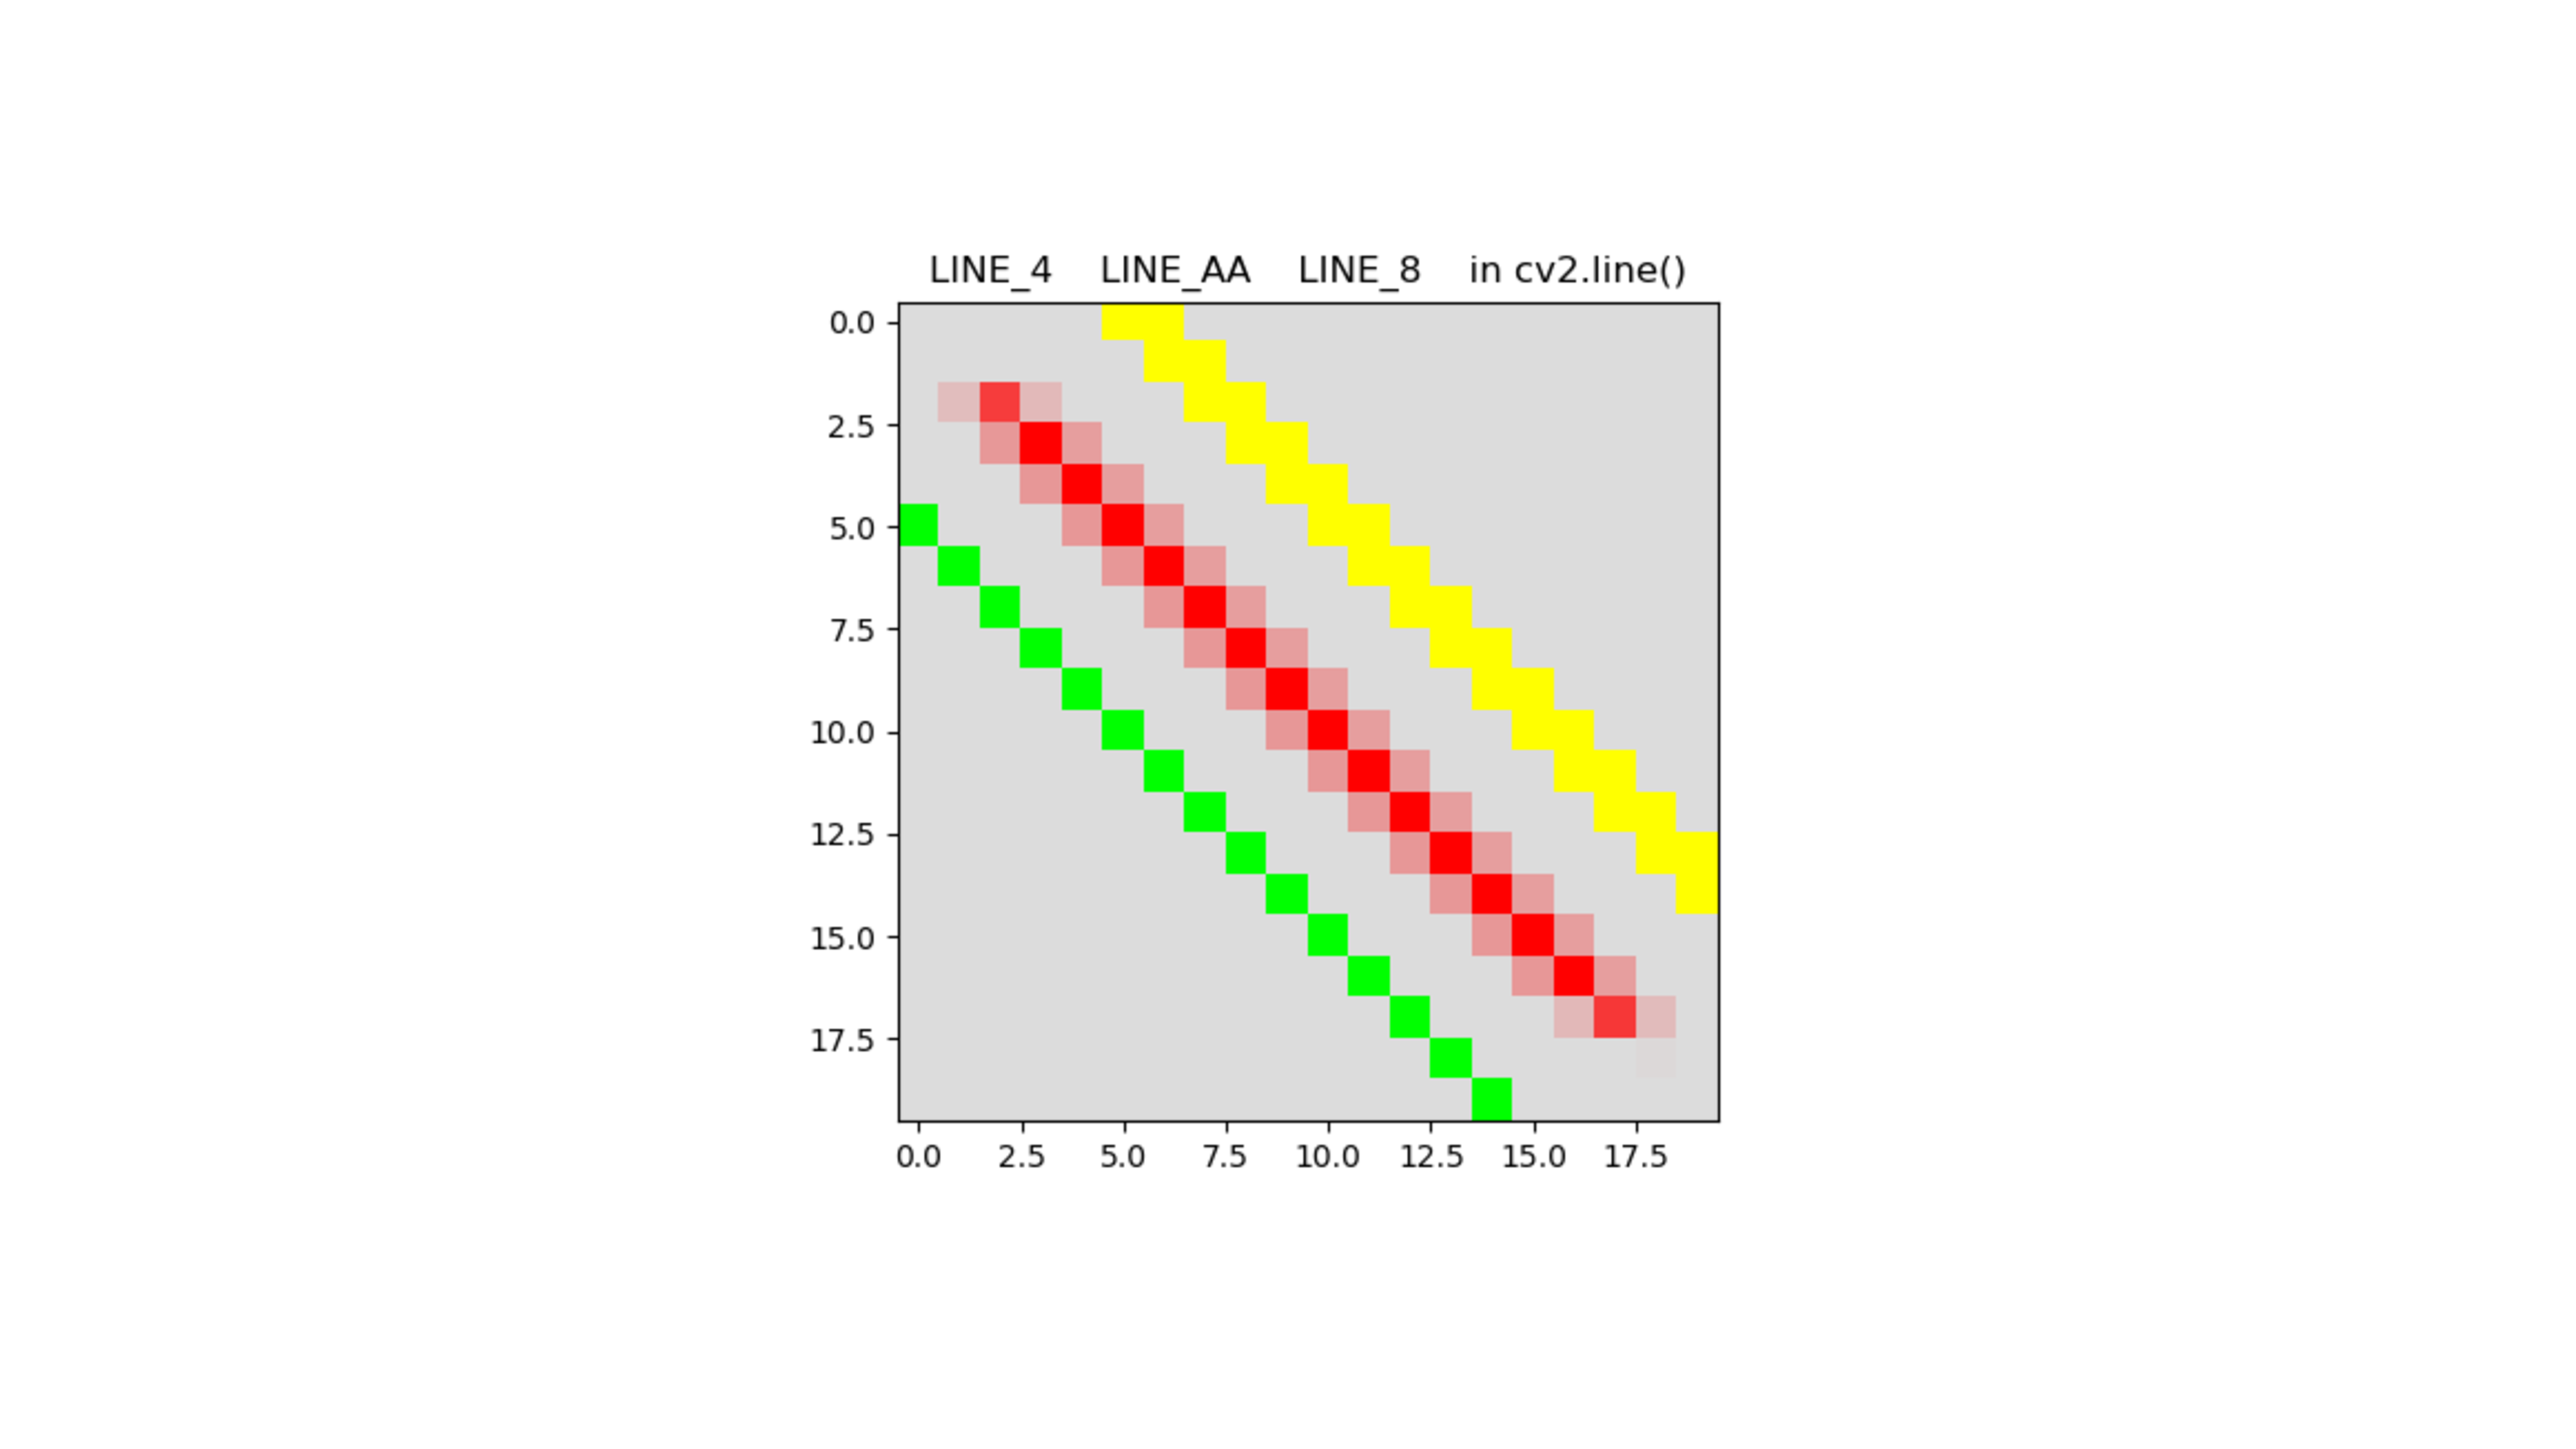
\includegraphics[width=0.4\linewidth]{LateX//figs/polyline.pdf}
        \caption{Example of line representation using anti-aliasing. The red line demonstrates how this approach encodes both the exact location of the boundary and regions with probabilities greater than zero, according to grid's resolution.}
        \label{fig:polylines}
    \end{figure}
    \end{minipage}
    \vspace{0.25 cm}

    This method ensures smooth and precise boundary representation, as illustrated in Figure~\ref{fig:hd-map-boundaries}.
    
    \begin{minipage}{\linewidth}
    \begin{figure}[H]
        \centering
        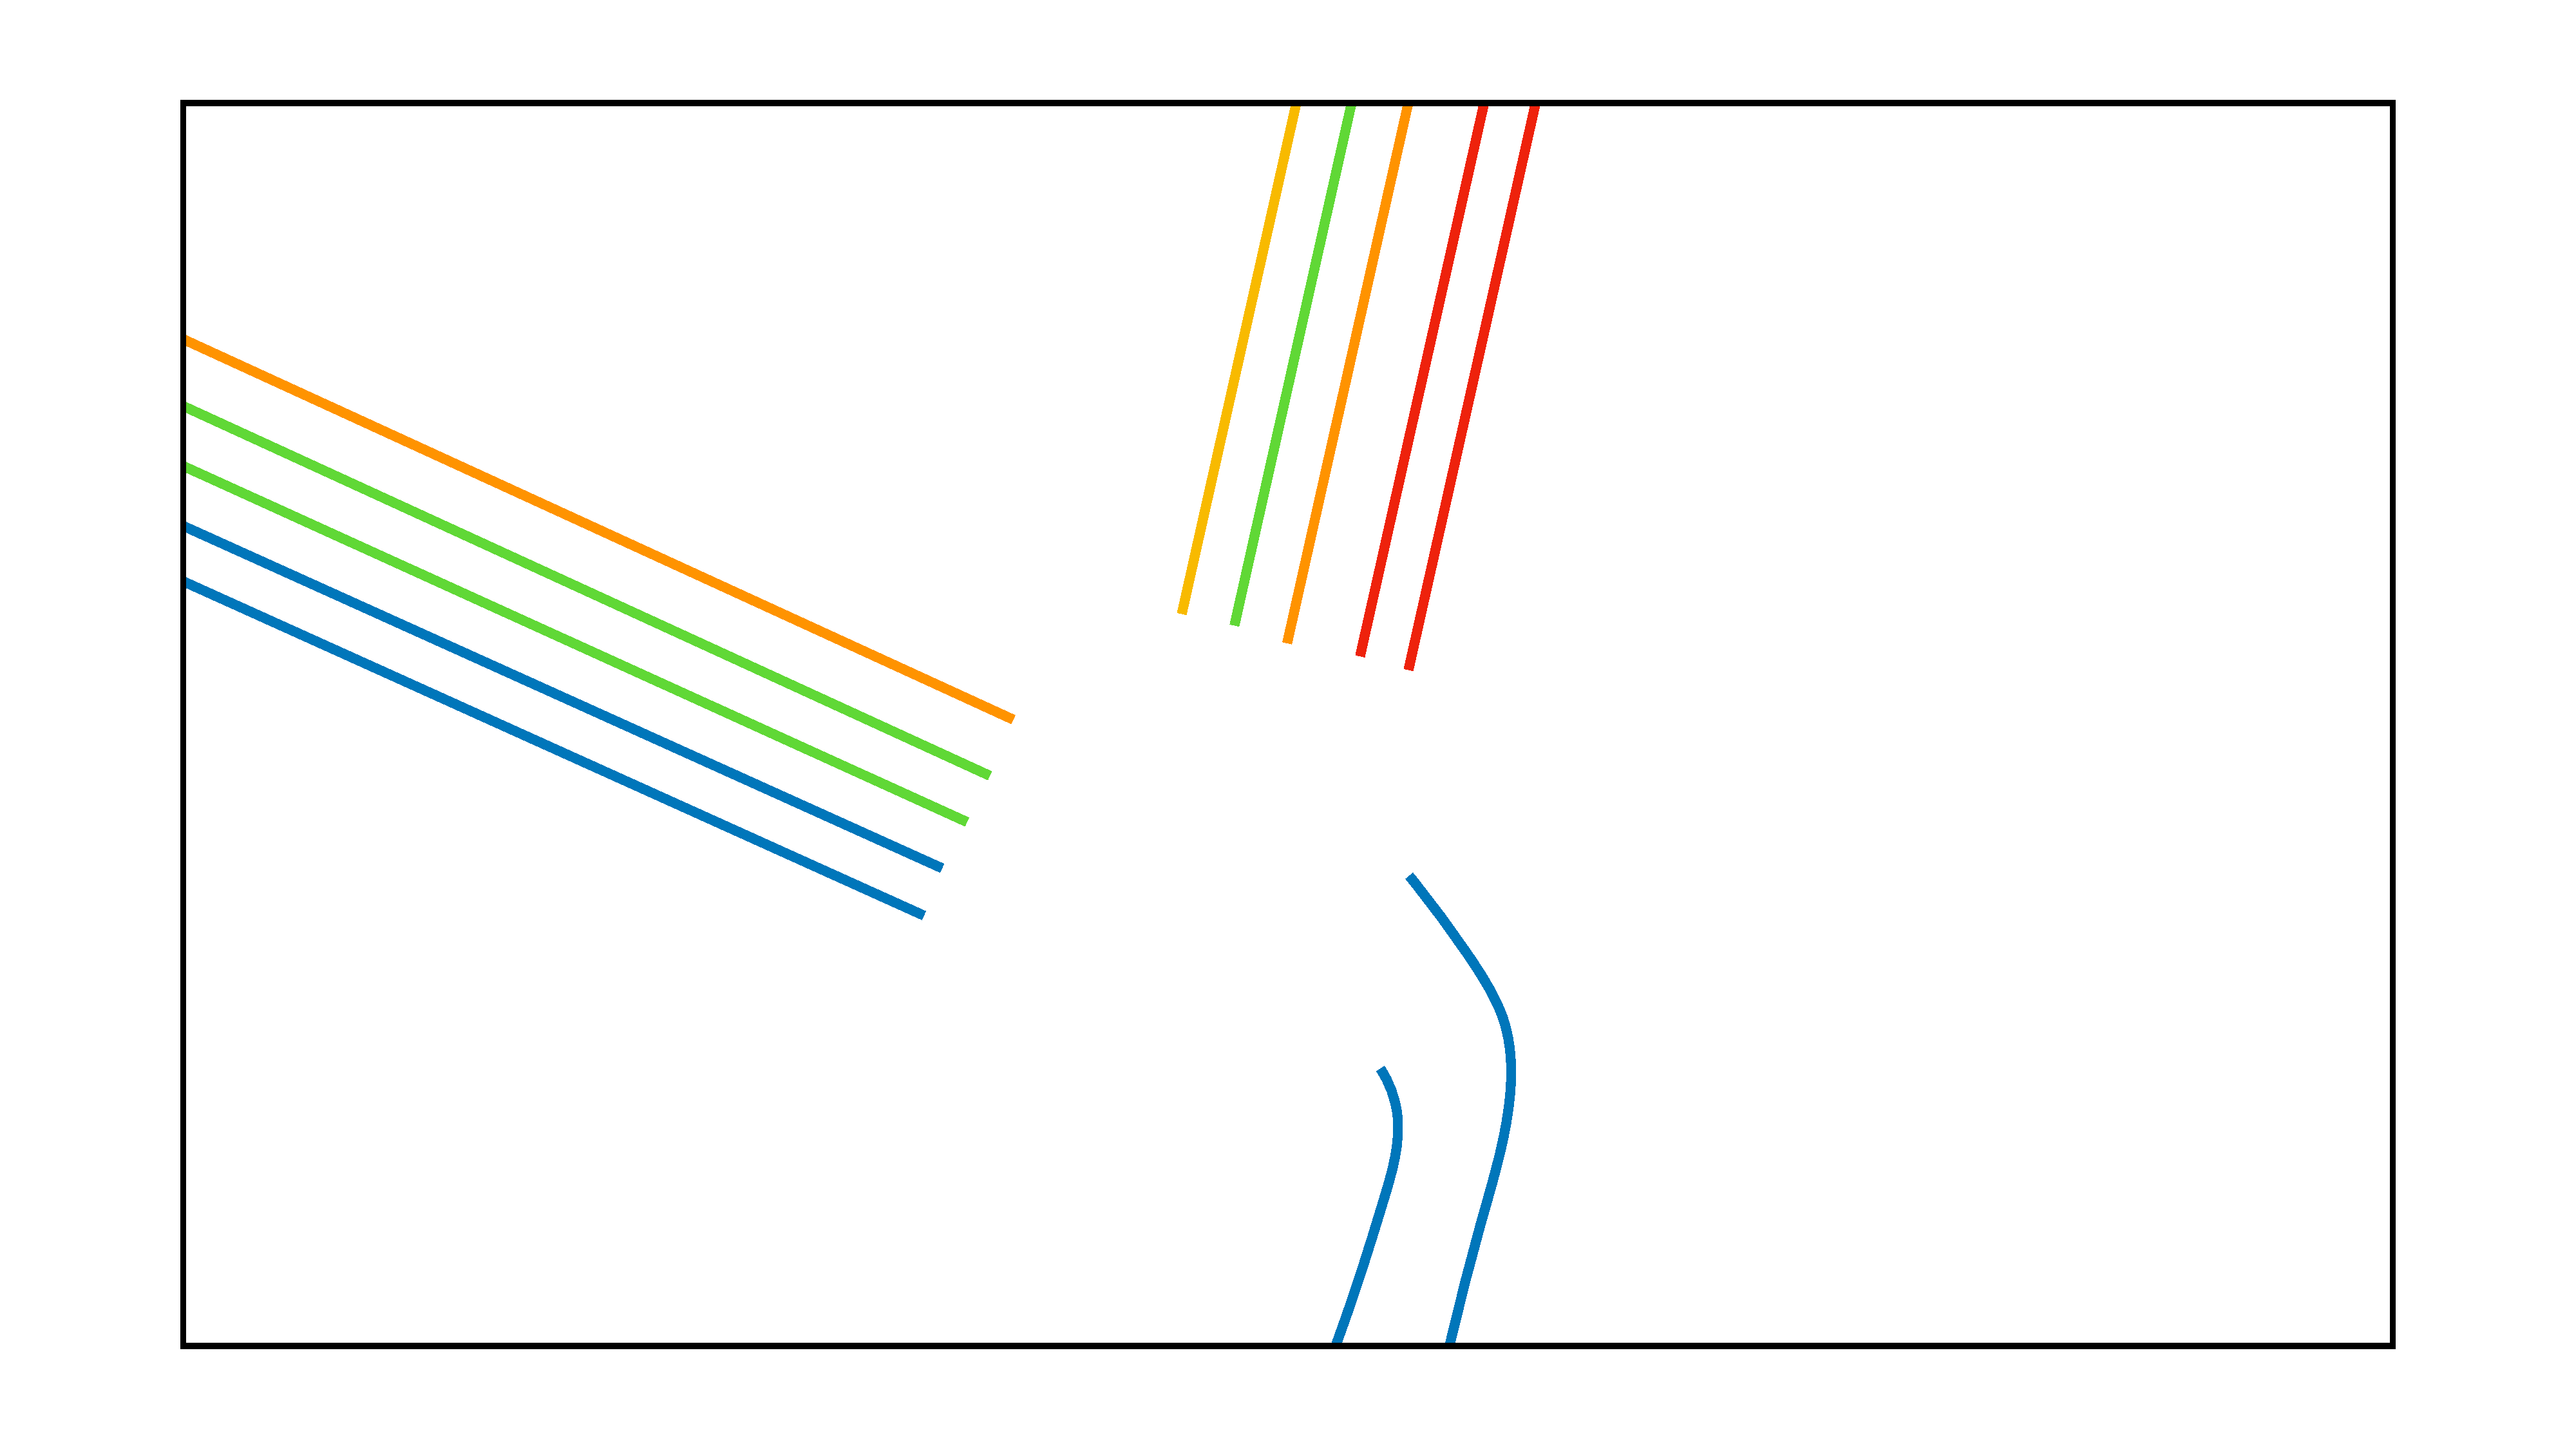
\includegraphics[width=0.9\linewidth]{LateX//figs/boundaries-mappahd.pdf}
        \caption{Tensor representation of all boundaries in the queried zone: different colors are used to distinguish between segments.}
        \label{fig:hd-map-boundaries}
    \end{figure}
    \end{minipage}
    \vspace{0.25 cm}
    
    \item \textit{Texture Loader}: This loader is responsible for loading all images from the various cameras included in the sensor suite (which will be discussed in the following section). Each camera provides a unique view of the environment, capturing distinct visual information that the network can utilize for perception tasks.
    Historically, the term \textit{texture} was used in computer graphics to refer to images applied to 3D models or surfaces, giving them realistic visual details, such as color, pattern, and surface irregularities. 
    
    \begin{minipage}{\linewidth}
    \begin{figure}[H]
        \centering
        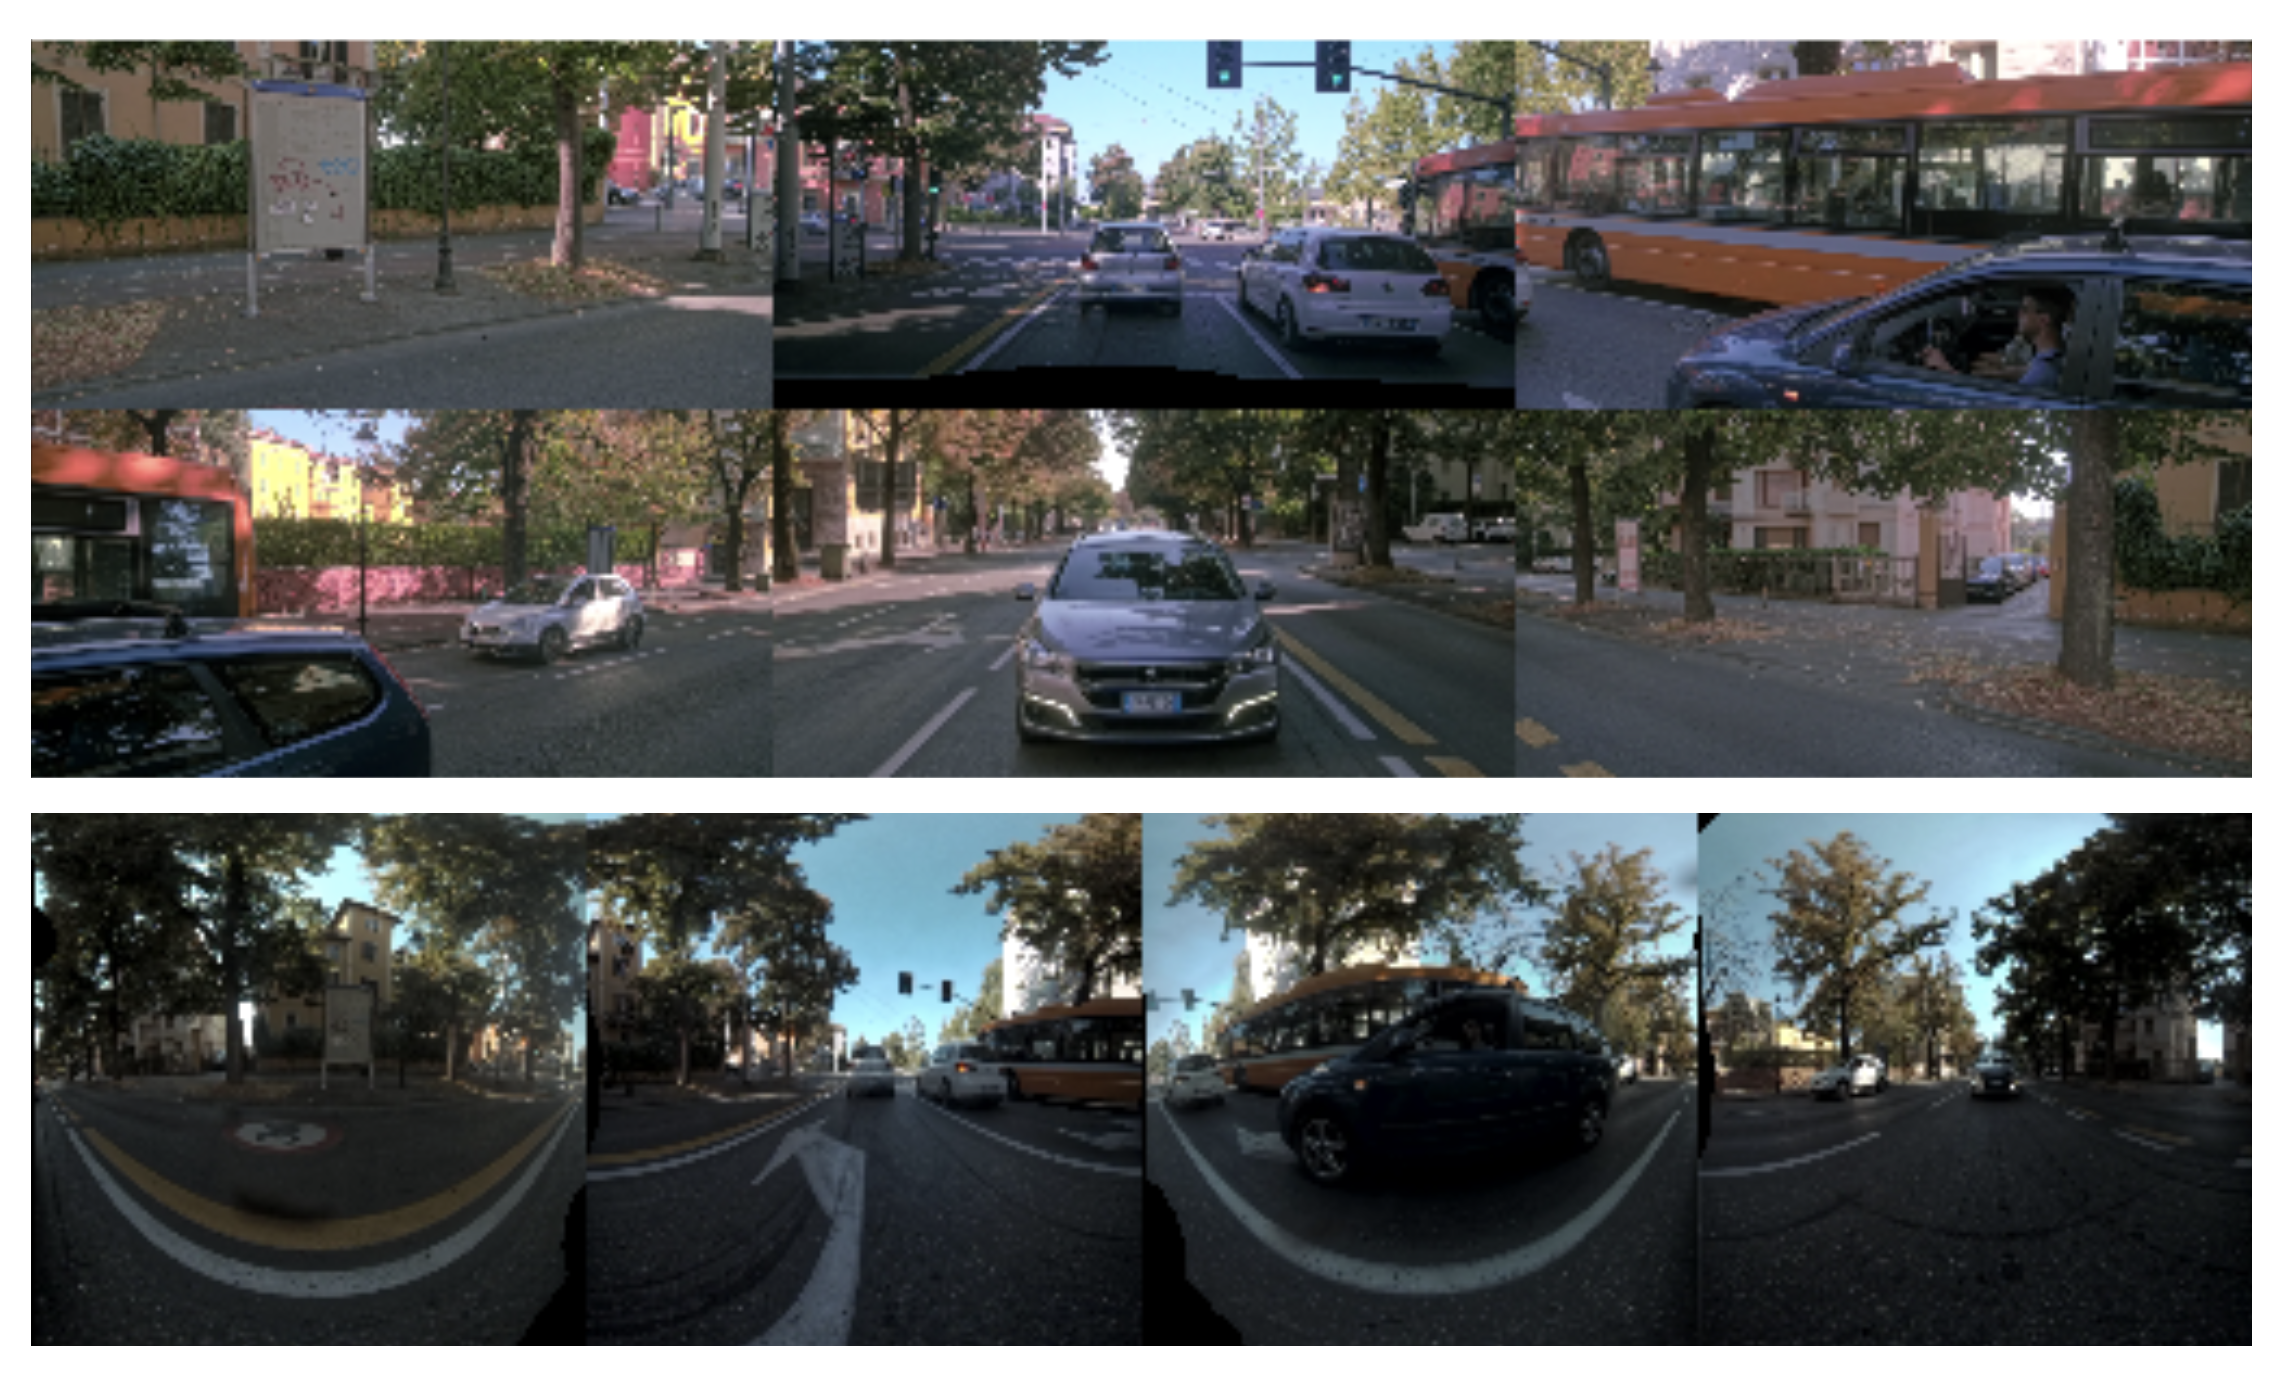
\includegraphics[width=0.95\linewidth]{LateX//figs/Screenshot 2024-09-27 at 12.00.55.png}
        \caption{Camera Textures: Images from Multiple Views. The first six images represent long-range cameras, while the last four correspond to short-range cameras.}
        \label{fig:texture-loader}
    \end{figure}
    \end{minipage}
    \vspace{0.25 cm}
    
    \item \textit{CamPosLoader:} This loader is responsible for loading all camera calibration data, including both intrinsic and extrinsic parameters, which are essential for accurately projecting the 3D environment onto a 2D image plane and aligning images for BEV (Bird's-Eye View) reconstruction.

    The \textit{intrinsic parameters} define the camera’s internal properties, which determine how 3D points are captured and transformed into 2D pixel coordinates. These parameters are represented by the intrinsic matrix \( A \), defined as:
    \begin{equation}
        A = \begin{bmatrix}
        k_uf_x & 0 & u_0 \\ 
        0 & k_vf_y & v_0 \\ 
        0 & 0 & 1 
        \end{bmatrix}
    \end{equation}
    where:
    \begin{itemize}
        \item \( f_x \) and \( f_y \) are the focal lengths in the \( x \) and \( y \) directions, typically measured in pixels.
        \item \( u_0 \) and \( v_0 \) are the coordinates of the principal point (optical center) on the image plane.
    \end{itemize}
    The intrinsic matrix \( A \) transforms 3D points in the camera’s local coordinate system into 2D pixel coordinates. Additionally, intrinsic parameters include distortion coefficients that correct lens distortions, ensuring the BEV projection remains geometrically accurate and undistorted.

    The \textit{extrinsic parameters} describe the camera's position and orientation relative to a fixed reference frame, often the vehicle's coordinate system. These parameters are represented by the rotation matrix \( R \) and the translation vector \( T \), which together form the extrinsic matrix \( [R \,|\, T] \):
    \begin{equation}
        [R \,|\, T] = \begin{bmatrix}
        r_{11} & r_{12} & r_{13} & t_x \\ 
        r_{21} & r_{22} & r_{23} & t_y \\ 
        r_{31} & r_{32} & r_{33} & t_z 
        \end{bmatrix}
    \end{equation}
    where:
    \begin{itemize}
        \item \( R \) is a \( 3 \times 3 \) rotation matrix that defines the camera’s orientation relative to the reference frame.
        \item \( T = \begin{bmatrix} t_x & t_y & t_z \end{bmatrix}^T \) is the translation vector, representing the camera’s position within the reference frame.
    \end{itemize}

    To project a 3D point from the world coordinate system onto the 2D image plane, the following transformation is applied:
    \begin{equation}
        \tilde{m} = A [R \,|\, T] \tilde{W}
    \end{equation}
    where:
    \begin{itemize}
        \item \( \tilde{W} = \begin{bmatrix} X & Y & Z & 1 \end{bmatrix}^T \) represents a 3D point in homogeneous coordinates in the world coordinate system.
        \item \( [R \,|\, T] \) transforms the 3D point from the world coordinate system into the camera's local coordinate system.
        \item \( \tilde{m} = \begin{bmatrix} u & v & 1 \end{bmatrix}^T \) represents the resulting 2D pixel coordinates in homogeneous form.
    \end{itemize}

    \item \textit{DirVector Loader:} This loader computes and provides the unprojected image coordinates, specifically the direction vectors from the camera's origin to the image plane at a normalized depth of 1. These direction vectors represent the world coordinates of each pixel as if projected onto a hypothetical image plane with a depth of 1, creating a unit depth field.
    
\end{itemize}

\subsection{Data Augmentation} 

Data augmentation is a technique used to artificially increase the diversity of training data by applying random transformations. This enhances the model’s ability to generalize to real-world variations not fully captured in the original dataset, making it more robust to unexpected changes in the input data \cite{MUMUNI2022100258}.

In this project, data augmentation is applied to simulate variations in the vehicle's position and orientation relative to the map. Using the optimized ground-truth position, known as \texttt{opt\_pose}, as the reference, augmentation introduces random rotations and shifts to mimic changes in the vehicle’s pose. This method accounts for slight discrepancies between the map alignment and the vehicle’s sensor data, preparing the model to handle similar disarrange during real-world application.

Specifically, the data augmentation, depicted in Figure~\ref{fig:data_augmentation_maps} involves:
\begin{itemize}
    \item \textit{Rotation}: The map is randomly rotated within a range of -$30$ to $30$ degrees to simulate orientation variations between the map and the vehicle.
    \item \textit{Translation}: The map is shifted horizontally and vertically by up to 10\% of the image’s width and height, respectively, to account for minor lateral and vertical misalignments. No translation is applied along the z-axis, as altitude is negligible for this scopes.

\end{itemize}

Directly using GNSS (Global Navigation Satellite System) data to align the map and vehicle pose can be problematic due to variability in GNSS accuracy. In some cases, GNSS data is highly accurate, providing near-perfect alignment with minimal adjustment effort. However, in other cases, GNSS data can be significantly inaccurate due to environmental factors like signal obstruction, leading to substantial misalignments. Relying just on GNSS data would result in an imbalanced dataset, with some examples well-aligned and others poorly aligned, which could negatively impact the training process.
\begin{figure}[H]
    \centering
    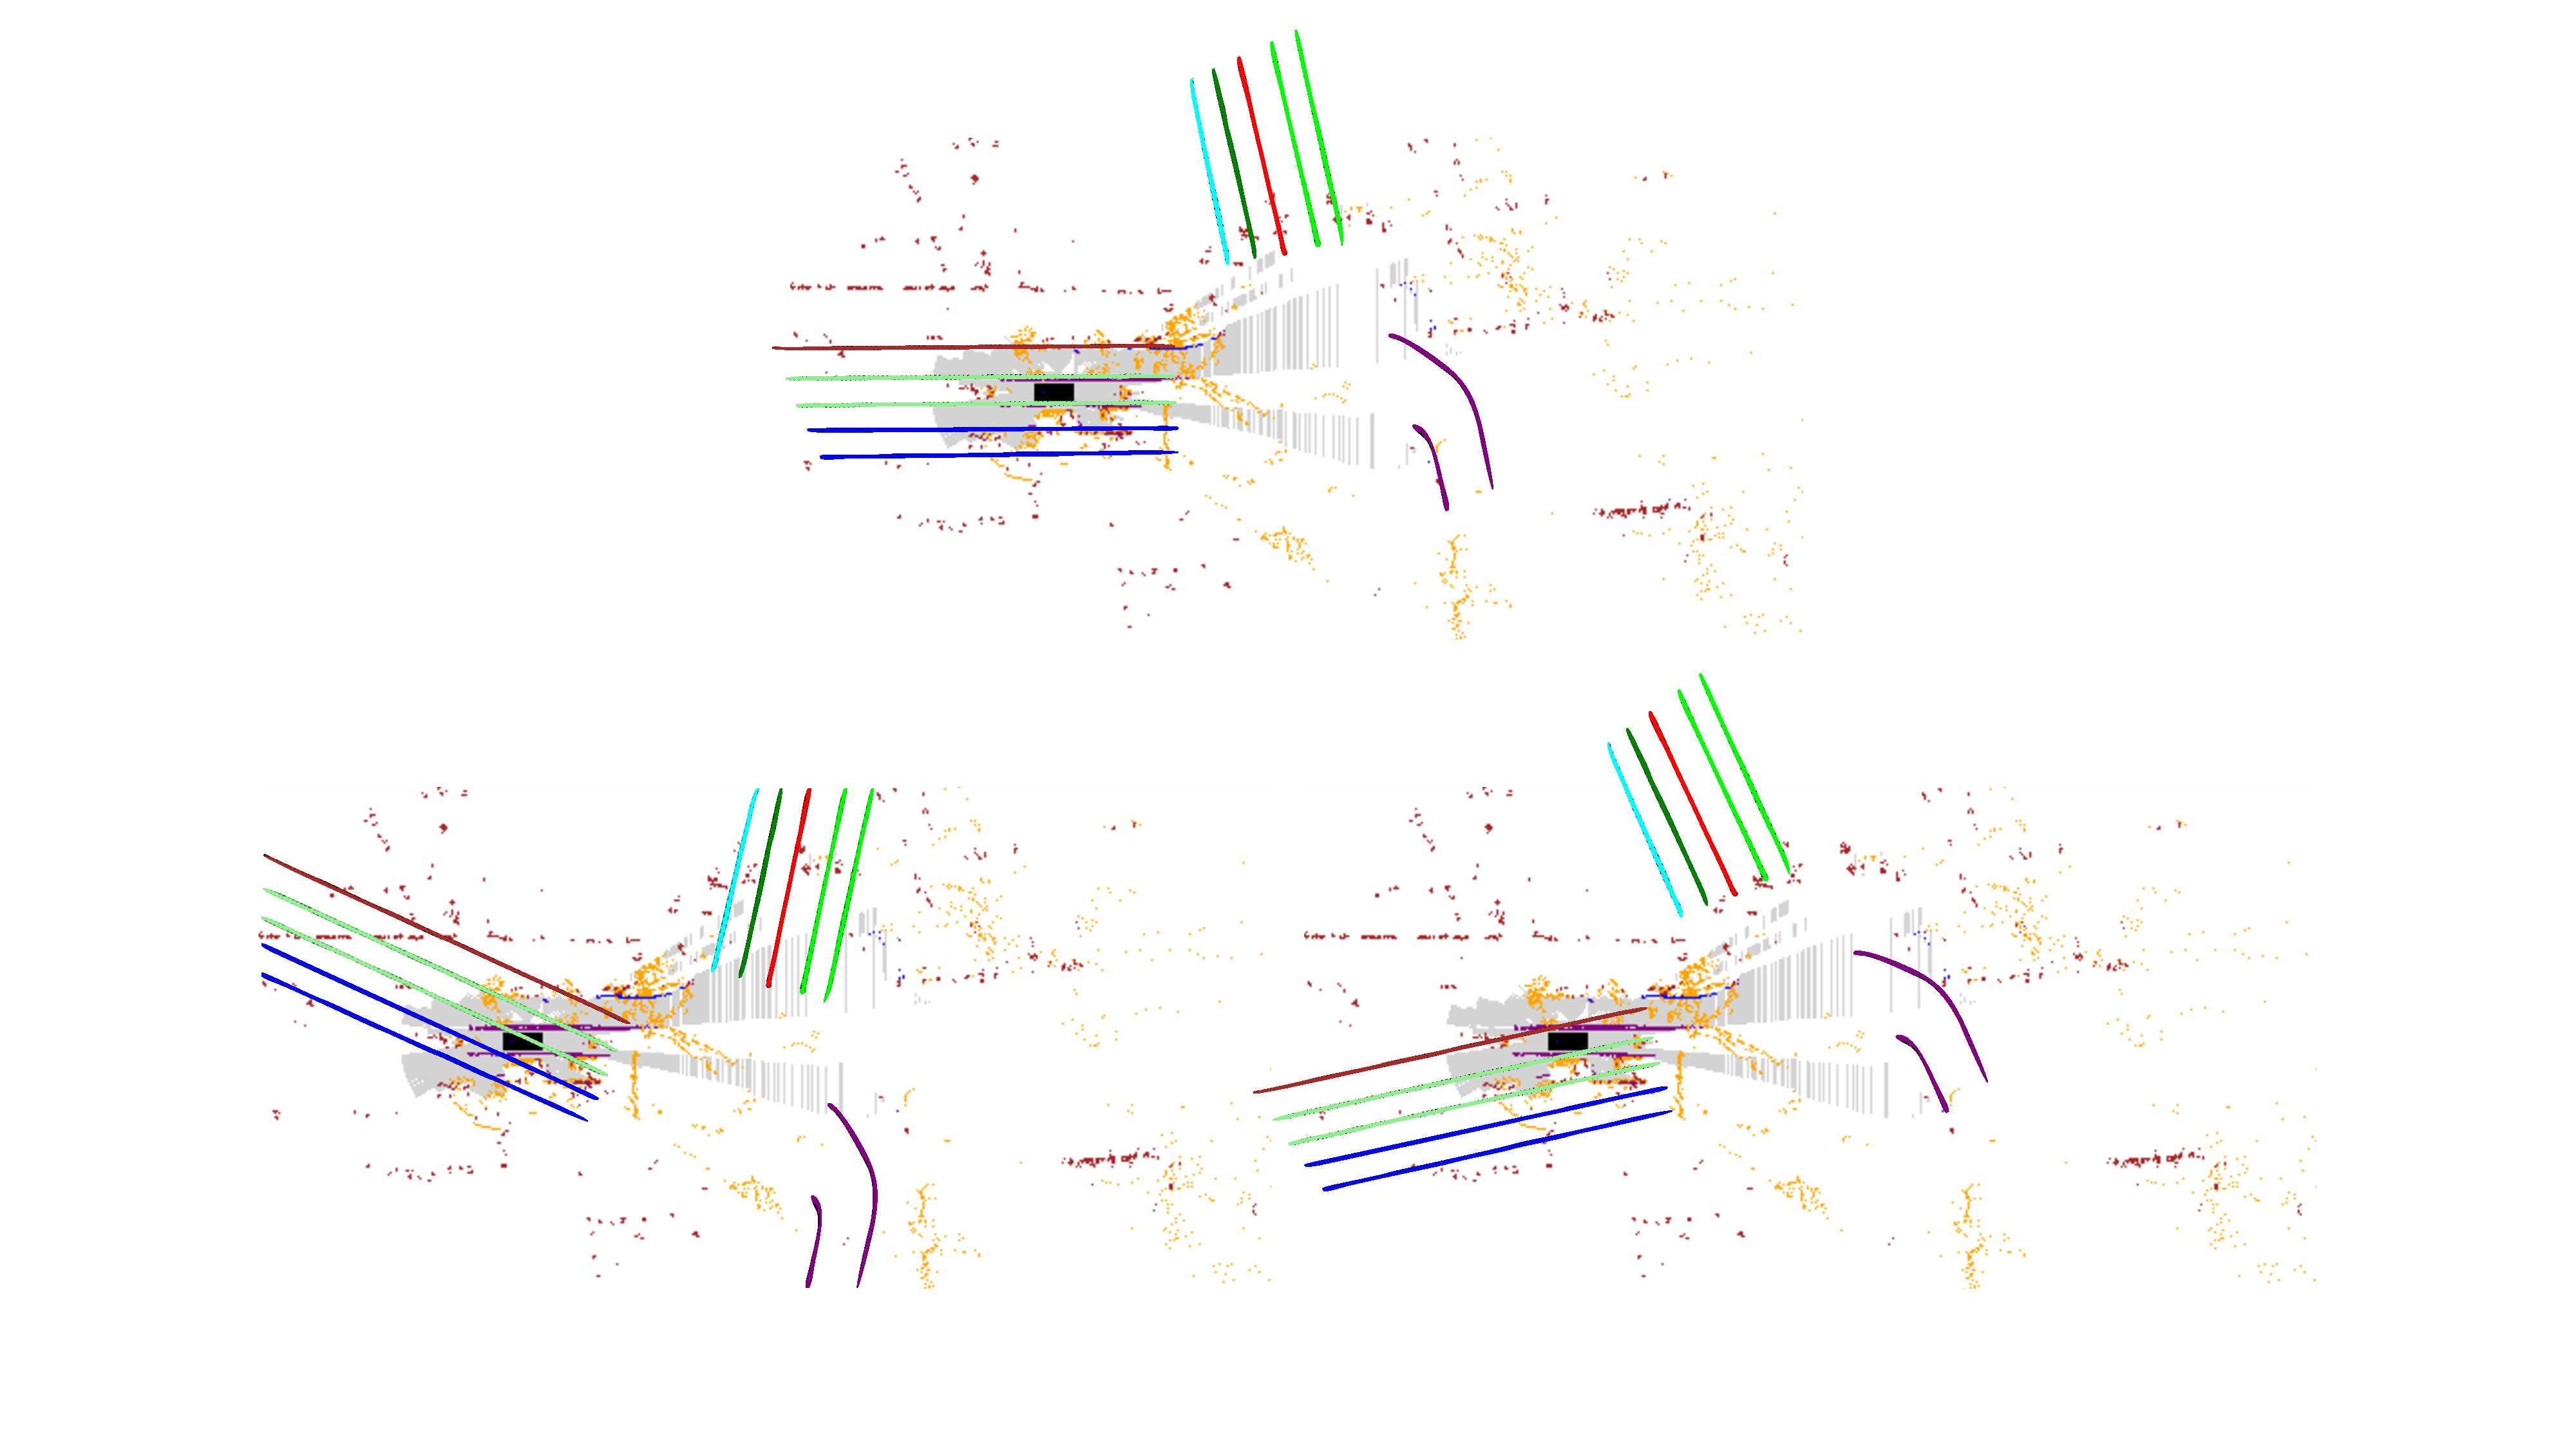
\includegraphics[width=1\linewidth]{LateX//figs/data_augmentation_zoom.pdf}
    \caption{Visual representation of various data augmentations applied to the same frame: different rotations and translations are demonstrated.}
    \label{fig:data_augmentation_maps}
\end{figure}
Using optimized positioning data that has been corrected through standard methods, a consistent and reliable ground-truth alignment is achieved, after which the previously described augmentation is applied, in order to get the most effective and well-balanced dataset possible.

In conclusion, all input loaders and data augmentation techniques have been described, detailing how each component contributes to the model's input preparation process. With these loaders and transformations in place, the network ultimately receives a well-structured and comprehensive input representation. This input integrates data from various sensors and includes augmented variations to ensure robustness, as illustrated in the figure below. The combined effect of these processes equips the network with diverse and realistic data, enhancing its ability to generalize in real-world applications.

\subsection{Target Loader}
The target loader is responsible for providing the target values that the network aims to predict. This loader prepares the ground-truth values for these transformations, giving the network a reference for learning to estimate spatial adjustments. In this context, the four values the network must predict include:
\begin{enumerate}
    \item Translation along the x-axis;
    \item Translation along the y-axis;
    \item Translation along the z-axis;
    \item Rotation around the vertical axis (yaw/heading angle).

\end{enumerate}
By learning these values, the network can effectively align the augmented data back to its original position, enhancing its robustness and accuracy in spatial localization.

\subsection{Post Processing}

As outlined in the previous subsection, the target is a set of four parameters: \( x \), \( y \), \( z \), and \( \theta \). These parameters define transformations between two primary reference frames: the world frame and the body-car frame. The transformation data can be computed either from the map to the car or vice-versa and are visualized accordingly.

Specifically, we focus on transformations between these two frames, as depicted in Figure~\ref{fig:post_processing}:
\begin{enumerate}
    \item \textbf{From World to Body Frame}: This transformation matrix, denoted as \( T_{W \to B} \), converts coordinates from the world frame (\( W \)) to the body (car) frame (\( B \)). It is defined as:
    \begin{equation}
        T_{W \to B} = \begin{bmatrix} 
        R_{W \to B} & t_{W \to B} \\ 
        0 & 1 
        \end{bmatrix}
    \end{equation}
    where:
    \begin{itemize}
        \item \( R_{W \to B} \): The \( 3 \times 3 \) rotation matrix aligning the world frame to the body frame orientation.
        \item \( t_{W \to B} \): The \( 3 \times 1 \) translation vector specifying the positional shift from the world frame to the body frame.
    \end{itemize}
    
    \item \textbf{From Body to World Frame (Inverse Transformation)}: To transform coordinates back from the body frame (\( B \)) to the world frame (\( W \)), the inverse transformation \( T_{B \to W} \) is used. It is calculated as:
    \begin{equation}
        T_{B \to W} = T_{W \to B}^{-1}
    \end{equation}
    Expanding this, the inverse transformation is given by:
    \begin{equation}
        T_{B \to W} = \begin{bmatrix} 
        R_{W \to B}^T & -R_{W \to B}^T \cdot t_{W \to B} \\ 
        0 & 1 
        \end{bmatrix}
    \end{equation}
    where:
    \begin{itemize}
        \item \( R_{W \to B}^T \): The transpose of the rotation matrix, reversing the rotation.
        \item \( -R_{W \to B}^T \cdot t_{W \to B} \): The transformed translation vector, adjusting the position back to the world frame.
    \end{itemize}
\end{enumerate}
\begin{figure}[H]
    \centering
    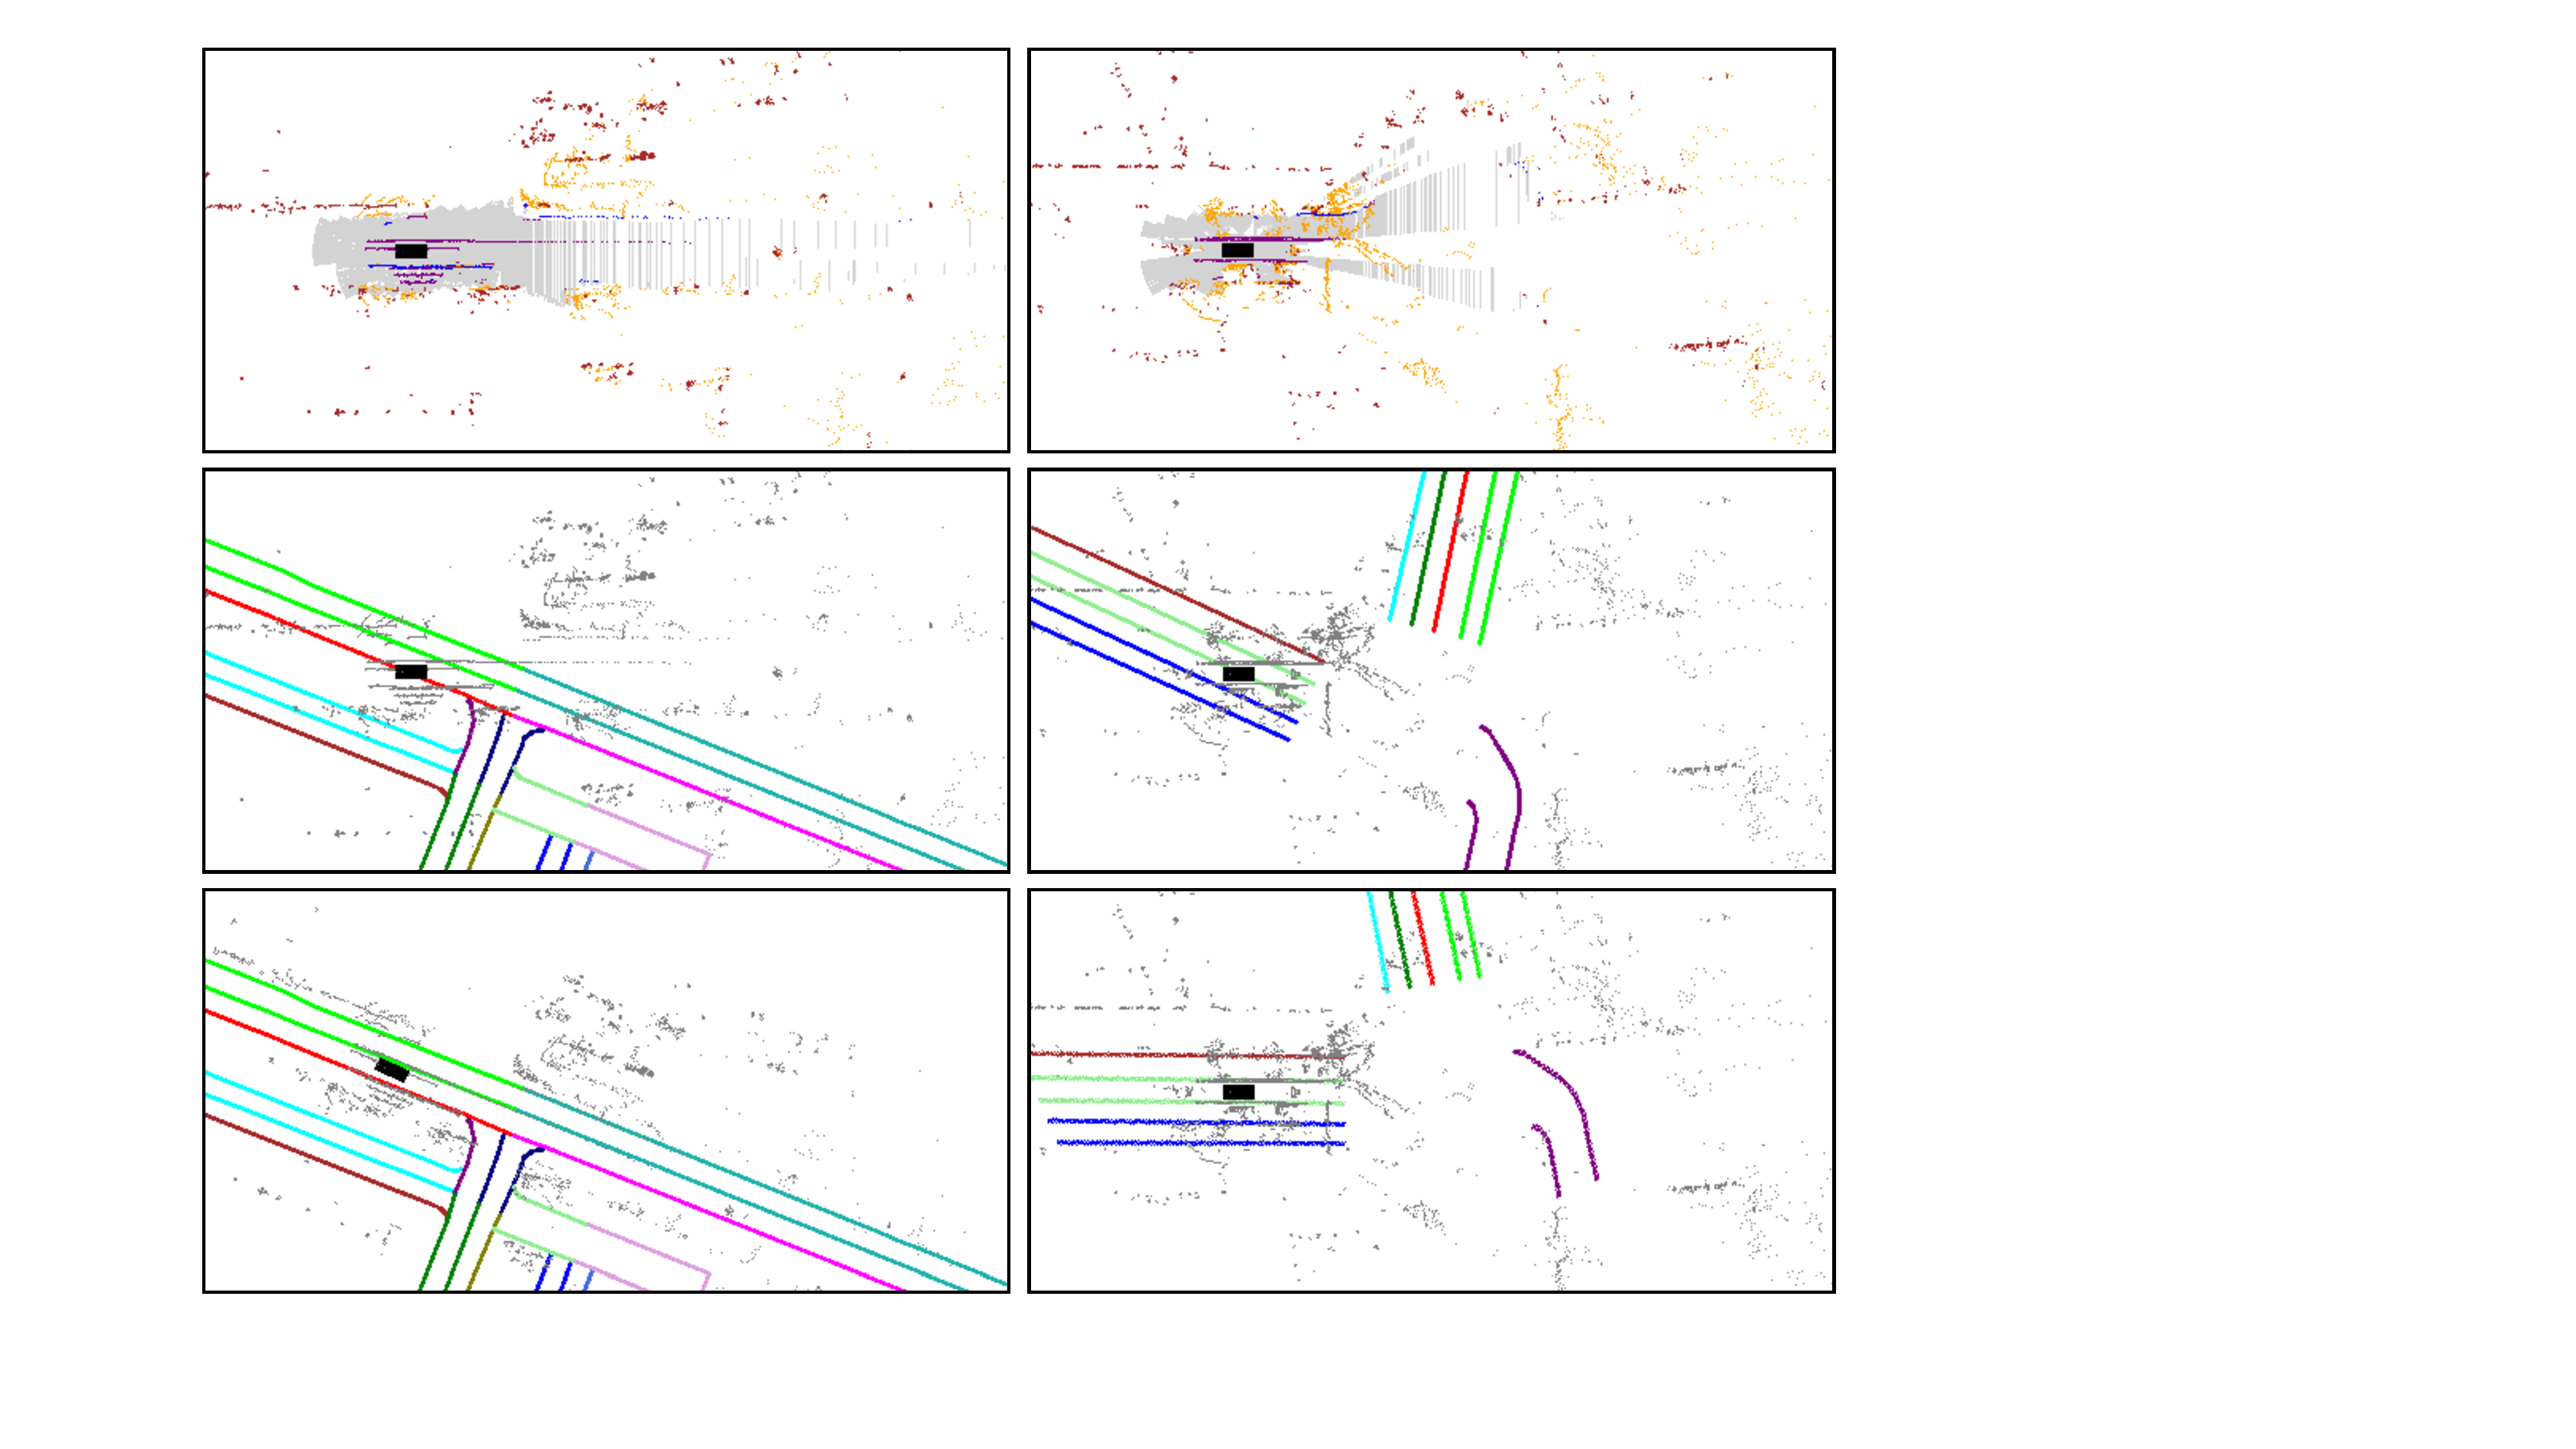
\includegraphics[width=0.85\linewidth]{LateX//figs/post_proc.pdf}
    \caption{The two images represent two different ways to process the output data: the roto-translation can be applied to the vehicle (right image) or to the map (left image).}
    \label{fig:post_processing}
\end{figure}

\section{Dataset}

The dataset comprises multiple sequences recorded in diverse urban environments, capturing a variety of driving conditions. Each frame in these sequences includes not only visual data but also synchronized information from all sensors mounted on the vehicle. The data is stored in an efficient \texttt{.bin} file format, optimizing storage and facilitating streamlined data handling. The dataset is collected from autonomous test vehicles equipped with a range of sensors, typically including:
\begin{itemize}
    \item Long-range cameras;
    \item Short-range cameras;
    \item Radars;
    \item GPS/GNSS.
\end{itemize}

\subsection{Sensor Suite}

The sensor suite configuration of the test vehicles integrates various sensors to provide a comprehensive perception of the environment. An illustration of the sensor suite configuration is shown in Figure \ref{fig:sensor-suite}. 
\begin{figure}[H]
    \centering
    \includegraphics[width=1\linewidth]{LateX//figs/carallview_compressed.pdf}
    \caption{Sensor suite representation: the front view and back view of the equipment, along with a BEV representation of the sensor mounting positions. Orange indicates the long-range stereo camera, green represents radar (mid-range or long-range), yellow appoints short-range stereo camera, and blue denotes the GNSS-IMU sensor.}
    \label{fig:sensor-suite}
\end{figure}

The long-range cameras can be used either as stereo cameras or mono cameras, depending on the type of test being conducted. In the specific sequences used for this project, data is sourced from six stereo cameras with a $70$-degree field of view. These cameras capture images at a resolution of $3840 \times 1920$ pixels and are used at a scale of $2$ (i.e., their dimensions are halved through pyramid scaling). This down-scaling facilitates faster inference operations by reducing computational load while retaining essential visual information.

Short-range cameras are positioned lower on the vehicle to enable a $360$-degree reconstruction of the environment around the car. After a de-warping process, these cameras capture images at a resolution of $992 \times 1024$ pixels, which are used at their full scale. Like the long-range cameras, they are stereo cameras but with a smaller baseline. This configuration allows for deterministic and traditional depth measurements of objects, making it easier to accurately position them within the world coordinates.

Pros of Using Stereo Cameras:
\begin{itemize}
    \item 3D Reconstruction: Stereo cameras enable the creation of 3D models and depth maps, providing a more comprehensive understanding of the scene by capturing spatial relationships between objects.
    \item Classification: The depth and location information from stereo images assist in classifying objects based on their three-dimensional positioning, enhancing object recognition capabilities.
\end{itemize}

Cons of Using Stereo Cameras:
\begin{itemize}
    \item Cost: Implementing stereo cameras requires double the hardware compared to mono cameras, and they demand powerful processing units to handle the increased data volume.
    \item Calibration Maintenance: Regular calibration is necessary to ensure accurate depth perception and alignment between the cameras. Any misalignment can lead to errors in depth estimation.
    \item Mechanical Challenges: Higher sensor resolutions in stereo setups can introduce mechanical complexities, such as the need for auto-calibration mechanisms to maintain alignment over time.
\end{itemize}

Another crucial set of sensors are radars, which offer different advantages and disadvantages compared to stereo cameras. Radars are less dependent on external lighting conditions, allowing for reliable object detection in various weather and lighting scenarios.

Radio Detecting and Ranging (RADAR) is a system used to detect the distance, angle, and speed of objects relative to the sensor. It operates by emitting radio or microwave signals using an array of antennas and capturing the signals that bounce back from objects in the environment. By processing these received signals, the system can extract the position, angle, and speed of targets.

The signal frequency used by radar systems can range from 1 to 110 GHz. Air traffic control applications require higher precision and thus use higher frequencies, while automotive applications typically use frequencies between 40 and 77 GHz. The time of flight for radar signals is approximately 6 microseconds per kilometer, allowing for rapid distance calculations. A frequency shift in the returned signal, known as the Doppler effect, is related to the speed of the target object.

Radar systems often employ a chirp or sweep signal—where the frequency increases or decreases over time—to improve the separation of targets and enhance resolution. Radars have been a consolidated technology in automotive applications for over 30 years, offering reliable performance even in adverse weather conditions. However, they may face challenges in detecting two closely spaced objects due to separation limitations.

Types of Automotive Radars:
\begin{itemize}
    \item Long-Range Radars: Capable of detecting objects up to 300 meters away, suitable for Adaptive Cruise Control (ACC) and highway driving scenarios.
    \item Medium-Range Radars: With a range of about $100$ meters, these are effective for detecting cross traffic, aiding in lane changes, and merging maneuvers.
    \item Short-Range Radars: Effective up to $30$ meters, ideal for low-speed maneuvers such as parking and navigating in tight spaces.
\end{itemize}

On the test vehicle, multiple radars are installed, including one long-range radar positioned at the front of the vehicle and several medium-range radars strategically placed to cover the surrounding environment.

At the conclusion of the dataset description, it is pertinent to highlight the specific areas of the city where the recorded sequences were collected. The data was gathered in various locations around Parma, including Via Langhirano, the train station area, and the Parma Fiere, as represented in Figure~\ref{fig:dataset_map}. These sequences comprise a total of [insert total frame count] frames, which were divided into training and validation sets to facilitate the model's development and evaluation.
\begin{figure}[H]
    \centering
    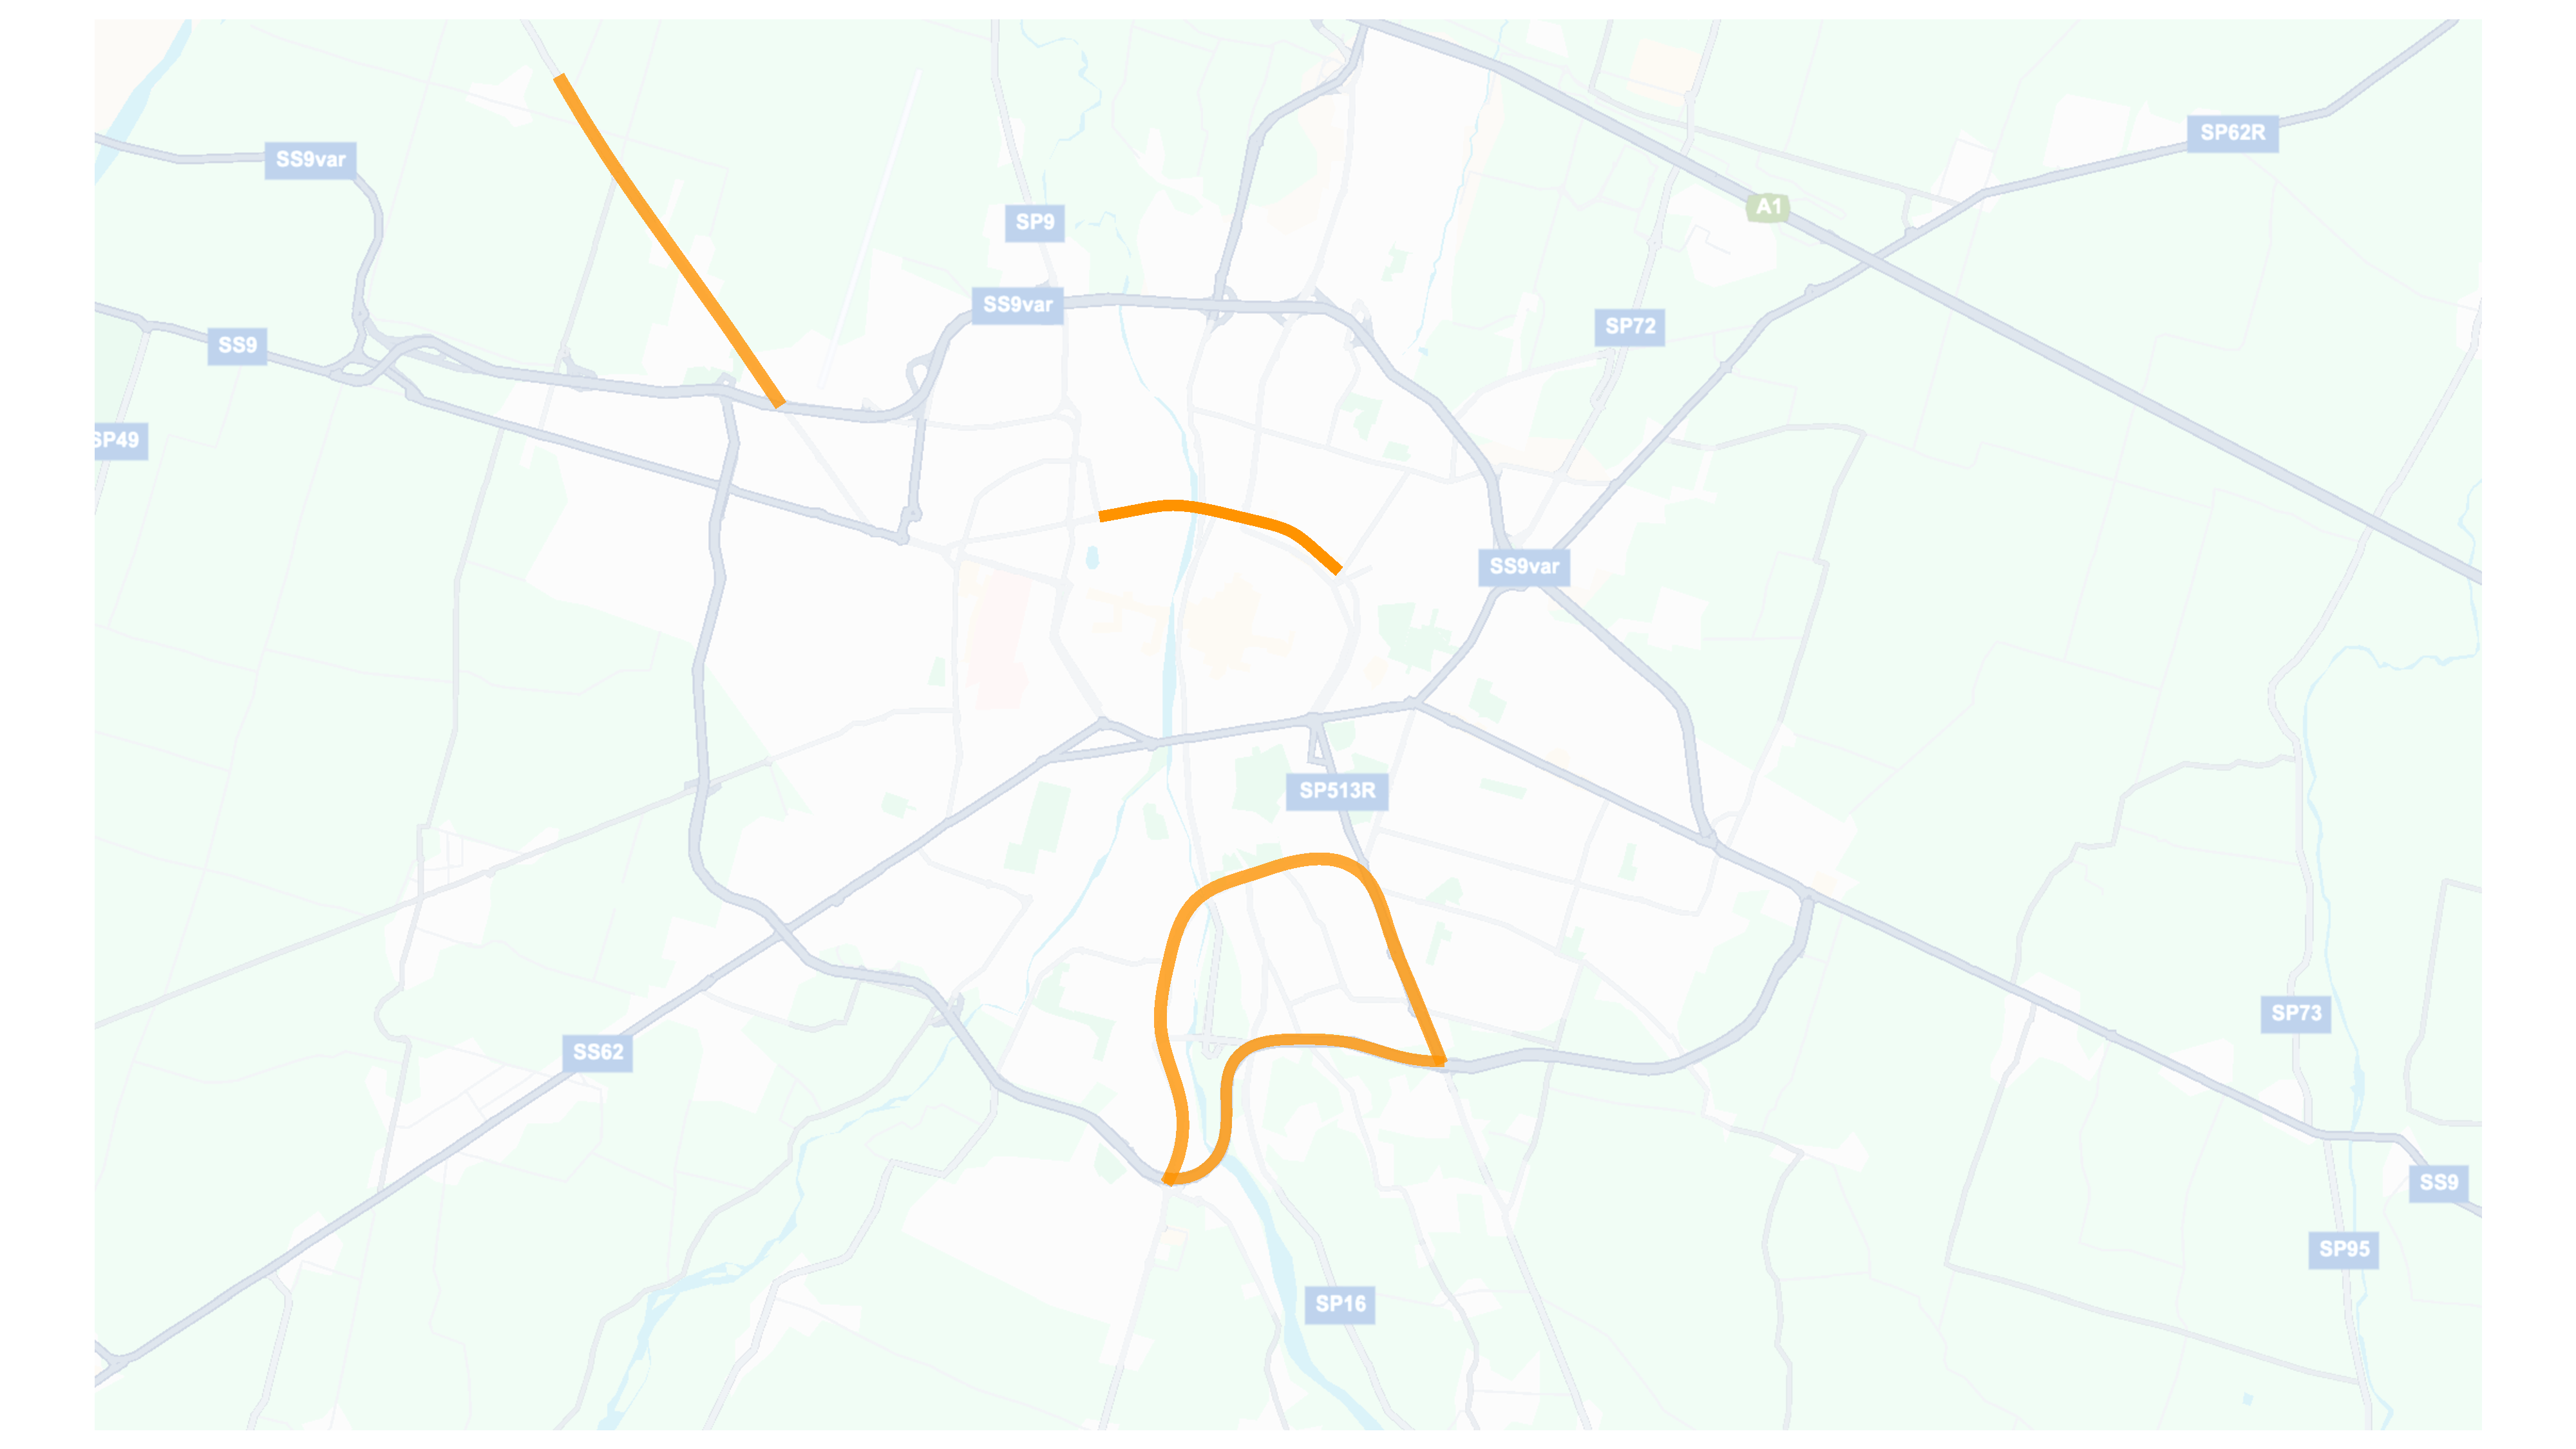
\includegraphics[width=0.9\linewidth]{LateX//figs/sequence_map.pdf}
    \caption{City representation with highlighted zones where the sequences were recorded.}
    \label{fig:dataset_map}
\end{figure}

During the project's development, two different dataset splits were utilized. Initially, only sequences from a specific area were used to reduce data volume and focus on refining the model's structure and functionality. This approach allowed for rapid iteration and debugging without the complexity of a large, diverse dataset. Once the foundational methodology was established and the optimal workflow was determined, the dataset was expanded to include all available recorded sequences. This expansion introduced greater diversity and complexity, enhancing the model's ability to generalize across different environments.

The dataset sequences incorporates a variety of scenarios captured under different weather and traffic conditions. Some sequences are captured without occlusions from other cars, while others are limited by a reduced horizon due to vehicles in front. There are sequences from both well-illuminated days and nighttime recordings, with varying illumination levels. This variation is critical because direct sunlight can cause reflections on camera lenses, rendering them ineffective. Similarly, at night, limited visibility can further restrict the field of view. Additionally, some sequences were recorded under adverse weather conditions, which contribute to the dataset’s robustness. In these cases, water droplets on the lenses can affect sensor performance. For instance, short-range cameras, positioned in the lower part of the vehicle, are particularly susceptible to being obstructed by water droplets.
\begin{figure}[H]
    \centering
    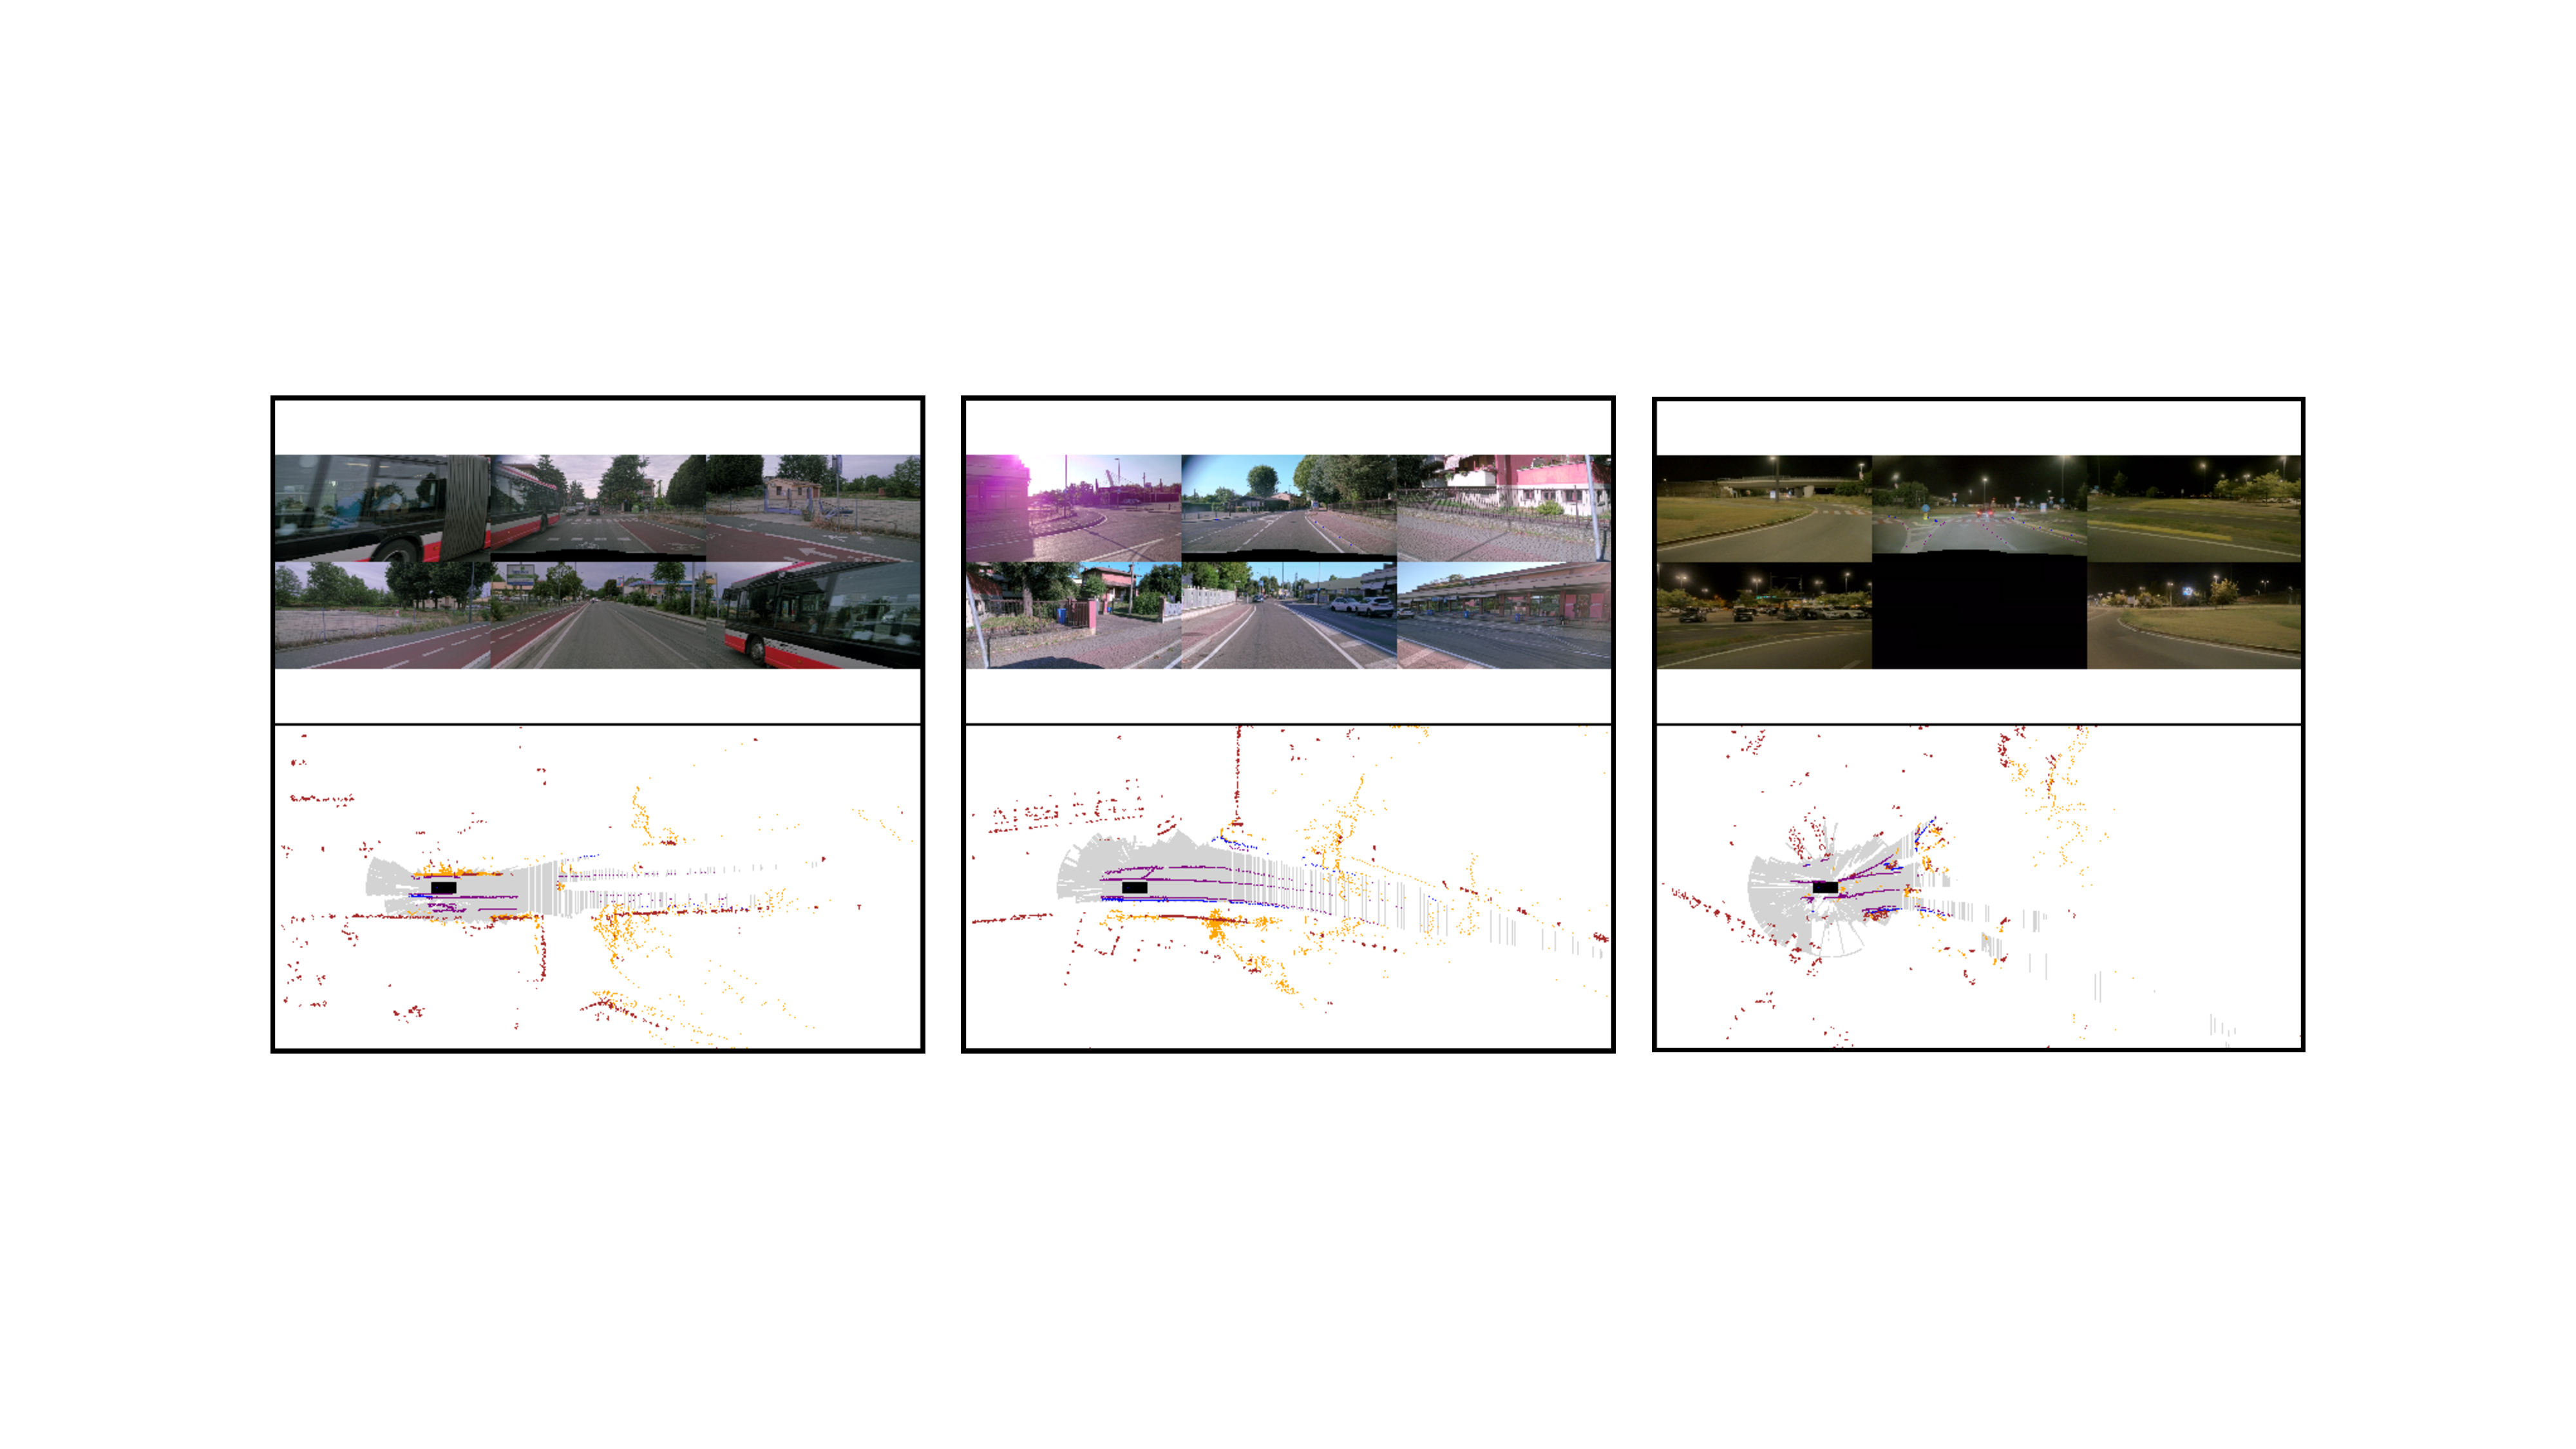
\includegraphics[width=1\linewidth]{LateX//figs/scenarios.pdf}
    \caption{Representation of different driving scenarios: obstructions, flare caused by direct sunlight, and nighttime sequences.}
    \label{fig:scenarios}
\end{figure}

Certain sequences also lack data from some cameras, a situation referred to as missing modalities. As shown in Figure~\ref{fig:missing_modalities}, this could occur if one of the long-range cameras was turned off or if a sequence was captured without the entire sensor suite dedicated to short-range cameras.
\begin{figure}[H]
    \centering
    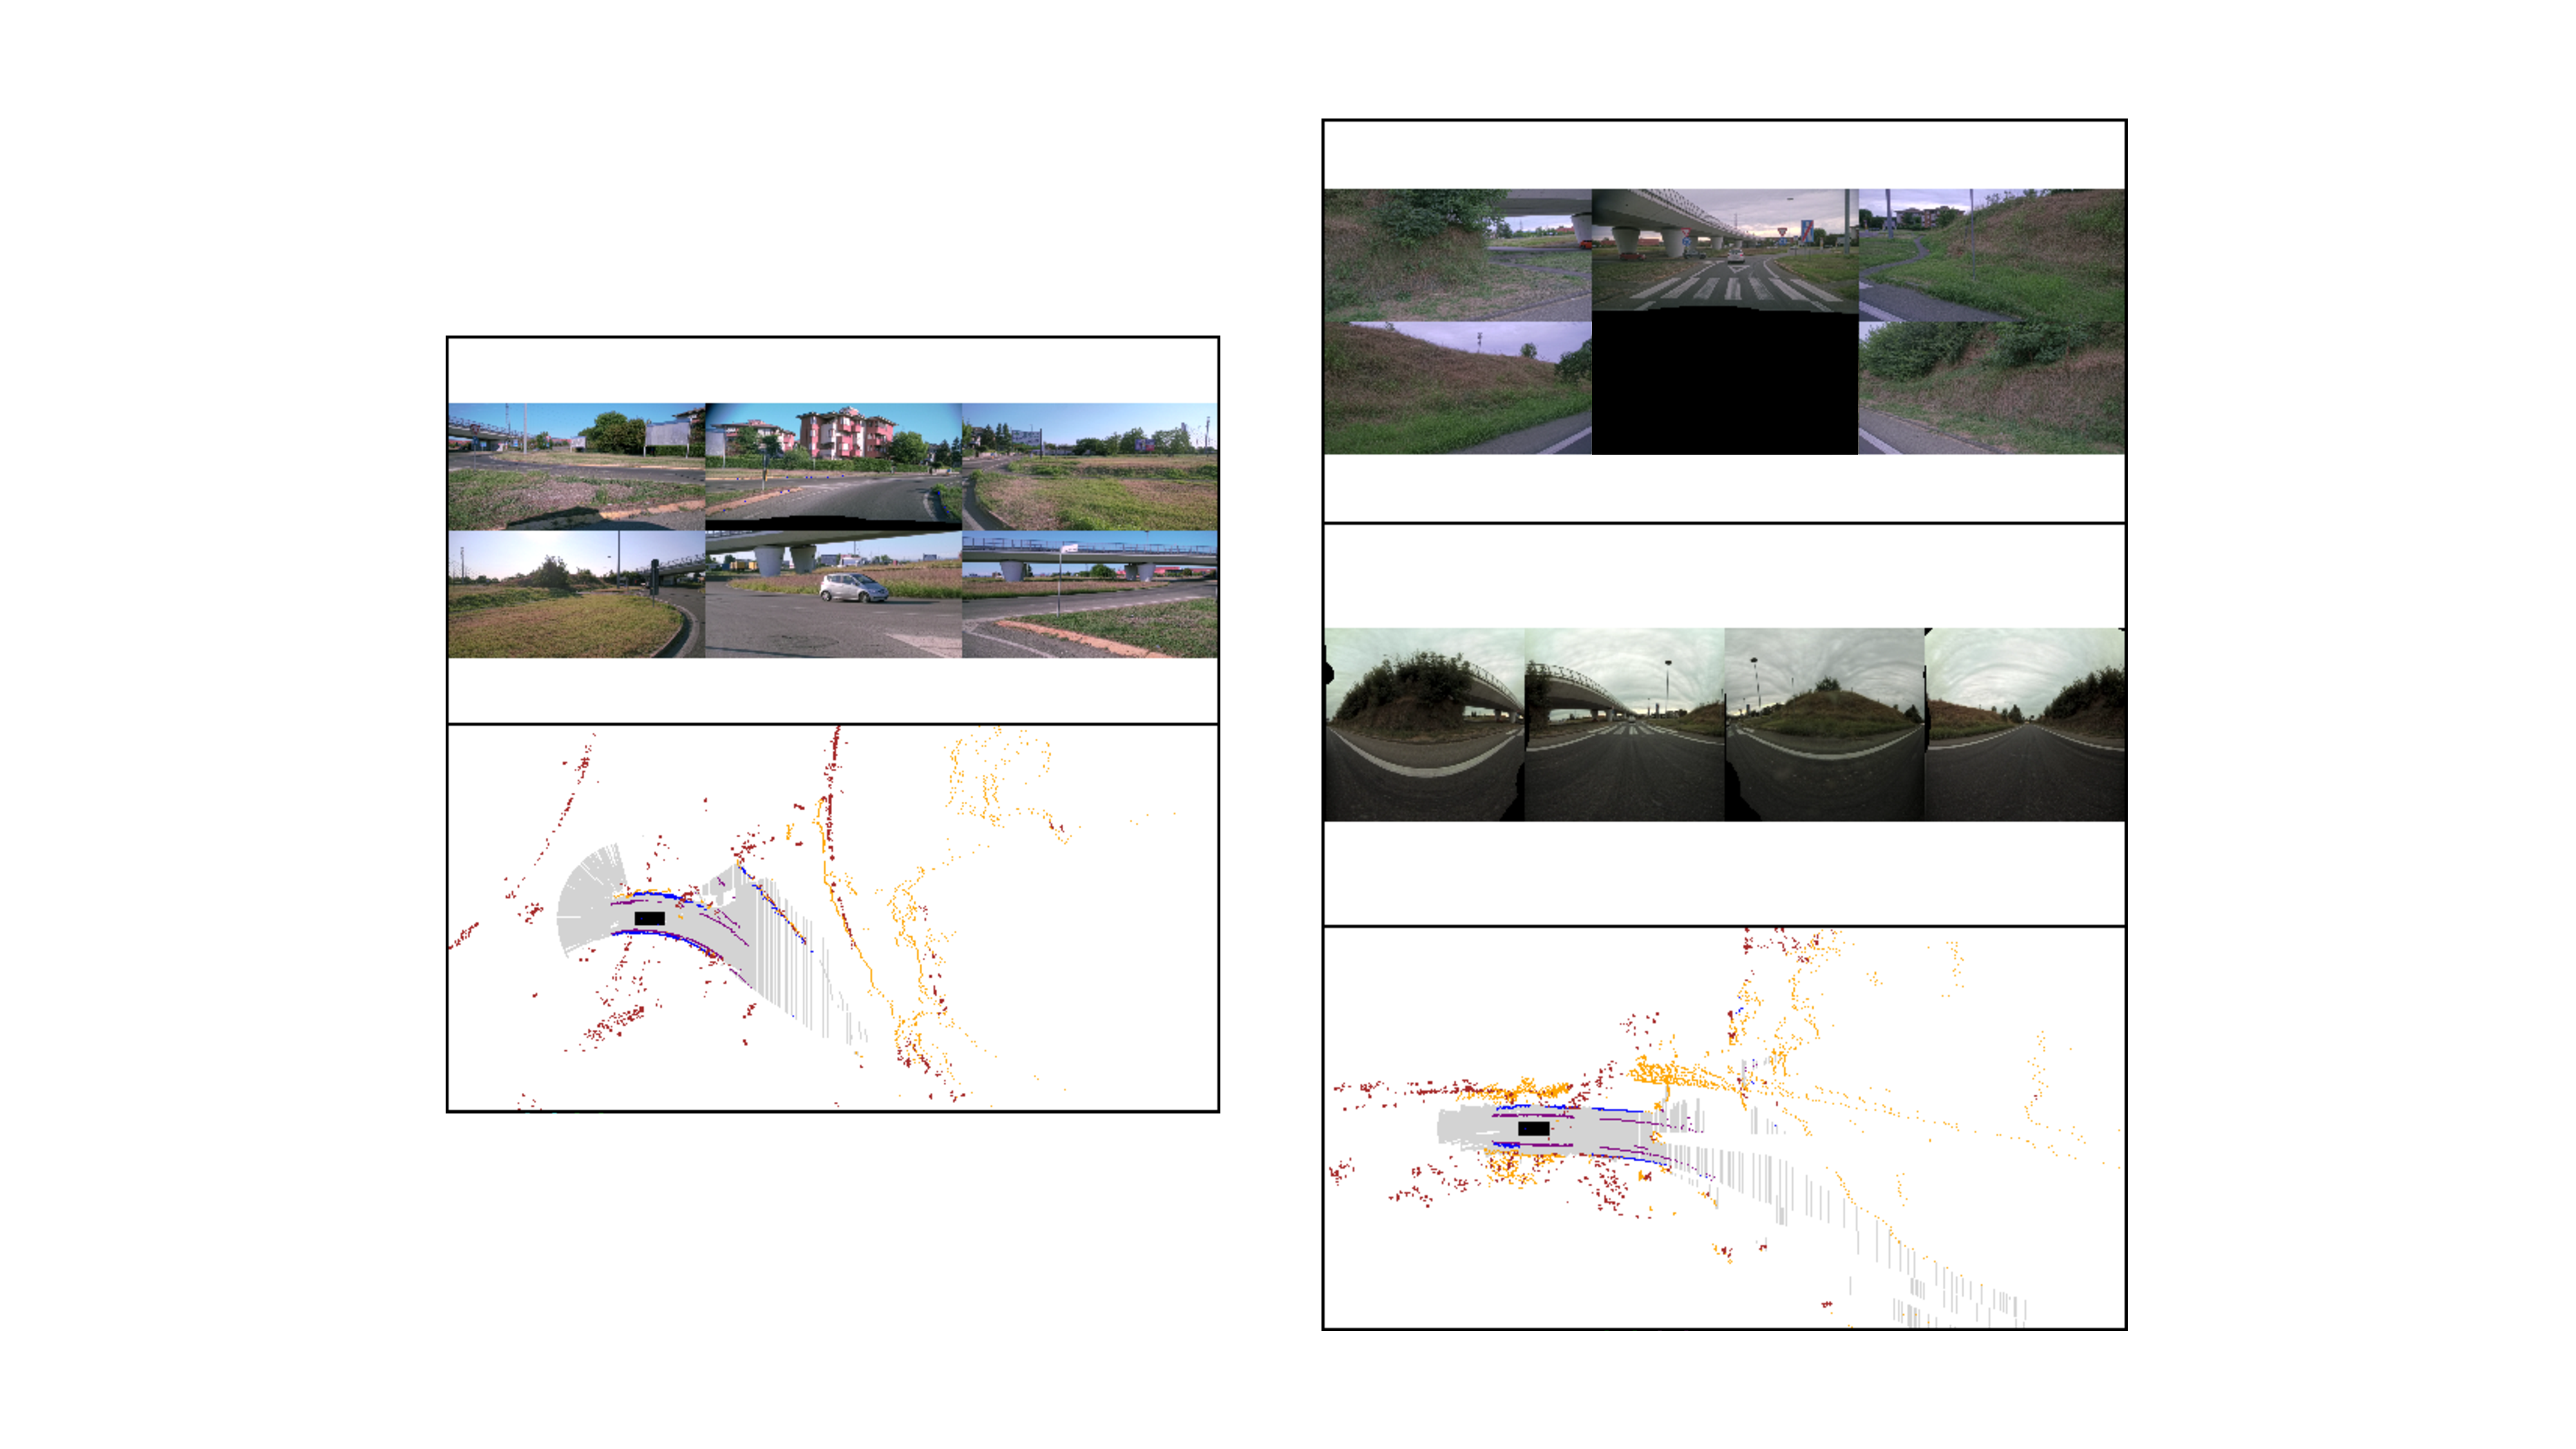
\includegraphics[width=0.6\linewidth]{LateX//figs/missing_modalities.pdf}
    \caption{Representation of missing modalities: in the left image, the short-range cameras were disconnected, while in the right image, one of the long-range cameras was out of use.}
    \label{fig:missing_modalities}
\end{figure}

All of these factors impact the detectors' ability to extract relevant environmental information, which in turn complicates the alignment process. 

\section{Methodology}

This section outlines the methodology employed to solve the task. After defining all the inputs and targets for the network and deserializing the required data, it is essential to describe the tools and frameworks utilized in the project. The model's detailed description and the various attempts made will be presented in the subsequent section.

The entire code-base was developed in Python, chosen for its compatibility with PyTorch, the primary tool used for the neural network implementation. \textit{PyTorch} is an open-source machine learning library developed by Facebook's AI Research lab (FAIR) in 2016 \cite{NEURIPS2019_9015}. It provides a flexible platform for deep learning research and production, emphasizing dynamic computation graphs and efficient tensor computations. PyTorch's use of tensors—multi-dimensional arrays similar to NumPy \cite{harris2020array} arrays but with support for GPU acceleration—makes it well-suited for the computational demands of deep learning tasks.

For training the neural network, \textit{CUDA} (Compute Unified Device Architecture) was employed to leverage GPU acceleration \cite{cuda}. CUDA is a parallel computing platform and programming model developed by NVIDIA, enabling dramatic increases in computing performance by harnessing the power of graphics processing units (GPUs). By utilizing CUDA, the code can perform parallel computations efficiently, significantly reducing training time and improving performance.

The training phase was conducted on a dedicated server equipped with three NVIDIA Tesla V100 GPUs, each with $32$ GB of memory, $256$ GB of RAM, and a $64$-core processor. Despite the availability of multiple GPUs, most of the training utilized a single GPU due to concurrent tasks that needed to be managed simultaneously. This setup provided the necessary computational resources to handle the intensive processing requirements of training deep neural networks.